\documentclass[aspectratio=169,12pt]{beamer}
\usepackage[utf8]{inputenc}
\usepackage{amsmath, amssymb}
\usepackage{booktabs}
\usepackage{colortbl}
\usepackage{hyperref}
\usepackage{makecell}
\usepackage{ragged2e}
\usepackage{bytefield}
\usepackage{tikz}
\usepackage[american]{circuitikz}
\usepackage{listings}
\usepackage{tcolorbox}
\usepackage{minted}
\usepackage[normalem]{ulem} % for strikethrough (\sout)
\usetikzlibrary{arrows.meta, positioning, shapes.geometric, calc, tikzmark, shapes.misc, backgrounds, matrix, shapes.callouts, fit, shapes.gates.logic.US}
\usetheme{Madrid}

% Define colors for BTB pipeline diagram (matching lecture_06)
\definecolor{myblue}{RGB}{0,0,255}
\definecolor{mygreen}{RGB}{0,128,0}
\definecolor{myorange}{RGB}{255,140,0}
\definecolor{lightgreen}{RGB}{144,238,144}
\definecolor{lightblue}{RGB}{173,216,230}
\definecolor{peach}{RGB}{255,218,185}
\lstset{
    escapeinside={@}{@},
    basicstyle=\ttfamily\small
}

\newcommand{\drawPipelineDiagram}[1][0,0]{%
    \scalebox{0.85}{%
    \begin{tikzpicture}[shift={(#1)},
        component/.style={draw, thick, minimum height=0.8cm},
        latch/.style={draw, thick, fill=yellow!20, minimum width=0.2cm, minimum height=4cm},
        stage/.style={font=\bfseries},
        label/.style={font=\tiny},
        port/.style={font=\tiny, inner sep=0.035cm},
        % Define styles for adder and muxes
        adder/.style={muxdemux, muxdemux def={Lh=4, NL=2, Rh=2, NR=1, NB=1, w=1.5, inset w=0.5, inset Lh=2, inset Rh=1.5}, 
                      external pins width=0, scale=0.4, fill=blue!15},
        greenmux/.style={muxdemux, muxdemux def={Lh=4, Rh=2, NL=2, NR=1, NB=0, NT=0, w=1}, 
                         external pins width=0, scale=0.6, fill=green!20},
        bluemux/.style={muxdemux, muxdemux def={Lh=2, Rh=4, NL=1, NR=2, NB=1, w=1}, 
                        external pins width=0, scale=0.6, fill=blue!20}
    ]
        % Define origin node for relative positioning
        \coordinate (origin) at (0,0);
        
        % Pipeline latches - positioned relative to origin with equal spacing
        \node[latch] (L1) at ([shift={(3,2)}]origin) {};
        \node[latch] (L2) at ([shift={(3,0)}]L1) {};
        \node[latch] (L3) at ([shift={(3,0)}]L2) {};
        \node[latch] (L4) at ([shift={(3,0)}]L3) {};
        
        % Stage labels - positioned at midpoints between latches
        \node[stage] at ([yshift=4cm]$(origin |- L1)!0.5!(L1)$) {Fetch};
        \node[stage] at ([yshift=4cm]$(L1)!0.5!(L2)$) {Decode};
        \node[stage] at ([yshift=4cm]$(L2)!0.5!(L3)$) {Execute};
        \node[stage] at ([yshift=4cm]$(L3)!0.5!(L4)$) {Memory};
        \node[stage] at ([yshift=4cm]$(L4.east) + (1.5,0)$) {WB};
        
        % Fetch Stage
        % PC MUX - blue mux should have right side wide (inputs), left side narrow (output)
        \node[bluemux] (pcmux) at ($(origin) + (0.3,4.5)$) {};
        \node[font=\tiny] at (pcmux.center) {};
        
        % Define PC MUX coordinates for compatibility
        \coordinate (pcmux_in1) at (pcmux.brpin 1);
        \coordinate (pcmux_in2) at (pcmux.brpin 2);
        \coordinate (pcmux_out) at (pcmux.blpin 1);
        \coordinate (pcmux_selectorup) at (pcmux.bbpin 1);

        % PC - positioned relative to L1
        \node[component, fill=blue!20, minimum width=0.6cm, minimum height=0.6cm] (PC) at ([xshift=-2.5cm, yshift=0]L1.center) {\small PC};

        % ICache - positioned relative to L1
        \node[component, fill=purple!20, minimum width=1.2cm, minimum height=2cm] (ICache) at ([xshift=-1cm, yshift=0]L1.center) {};
        \node[align=center] at ([yshift=0.6cm]ICache.center) {\footnotesize inst.\\[-0.14cm]\footnotesize cache};
 
        % PC adder using circuitikz with one bit adder style
        \node[adder] (fe_adder) at ($(PC.center) + (0.7,1.8)$) {};
        \node[font=\tiny] at (fe_adder.center) {+};
        \coordinate (fe_adder_input1) at (fe_adder.blpin 1);
        \coordinate (fe_adder_input2) at (fe_adder.blpin 2);
        \coordinate (fe_adder_output) at (fe_adder.brpin 1);
        \node[left, font=\tiny] (four) at ([xshift=-0.2cm]fe_adder_input1) {4};
        
        % Decode Stage - positioned between L1 and L2, with vertical offset
        \node[component, fill=pink!30, minimum width=1.2cm, minimum height=1.8cm] (RF) at ($(L1.east)!0.5!(L2.west) + (0,0.41)$) {};
        \node[align=center] at ([yshift=-0.35cm]RF.north) {\footnotesize register\\[-0.11cm]\footnotesize file};
        
        % Register file input ports (left side, inside the box)
        \node[port] (rf_src1) at ([xshift=-0.4cm, yshift=0.1cm]RF.center) {~src1};
        \node[port] (rf_src2) at ([xshift=-0.4cm, yshift=-0.3cm]RF.center) {~src2};
        \node[port] (rf_dst) at ([xshift=-0.35cm, yshift=-0.7cm]RF.center) {dst};
        
        % Register file selector coordinate (slightly left of dst)
        \coordinate (rf_selector) at ([xshift=-0.1cm]rf_dst.south);
        
        % Register file output ports (right side, aligned to right edge)
        \node[port, anchor=east] (rf_src1_data) at ([xshift=0.6cm, yshift=0.07cm]RF.center) {src1};
        \node[port, anchor=east] (rf_data1) at ([yshift=-0.15cm]rf_src1_data.east) {data};
        \node[port, anchor=east] (rf_src2_data) at ([xshift=0.6cm, yshift=-0.37cm]RF.center) {src2};
        \node[port, anchor=east] (rf_data2) at ([yshift=-0.15cm]rf_src2_data.east) {data};
        
        % Sign extension - positioned relative to register file  
        \node[component, fill=green!20, ellipse, minimum width=0.4cm, minimum height=0.3cm, align=center] (SignExt) at ([xshift=0.6cm, yshift=-1.5cm]RF.center) {
            \scriptsize sign\\[-0.25cm]\scriptsize ext.
        };
        
        % Execute Stage
        % Execute adder using circuitikz with one bit adder style
        \node[adder] (ex_adder) at ($(L2.east)!0.5!(L3.west) + (0,1.56)$) {};
        \node[font=\tiny] at (ex_adder.center) {+};
        \coordinate (ex_adder_input1) at (ex_adder.blpin 1);
        \coordinate (ex_adder_input2) at (ex_adder.blpin 2);
        \coordinate (ex_adder_output) at (ex_adder.brpin 1);
        
        % Execute stage ALU source MUX - green mux should have left side wide (inputs), right side narrow (output)
        \node[greenmux] (exemux) at ($(L2.east)!0.5!(L3.west) + (0,-0.32)$) {};
        \node[font=\tiny] at (exemux.center) {};
        \coordinate (exemux_in1) at (exemux.blpin 1);
        \coordinate (exemux_in2) at (exemux.blpin 2);
        \coordinate (exemux_out) at (exemux.brpin 1);
        
        % ALU using circuitikz ALU style
        \node[muxdemux, muxdemux def={Lh=5, NL=2, Rh=2, NR=1, NB=2, NT=1, w=2, inset w=1, inset Lh=2, inset Rh=0, square pins=1},
              external pins width = 0, scale=0.5, fill=green!15] (ALU) at ($(L2.east)!0.65!(L3.west) + (0,0)$) {};
        \node[rotate=90, font=\tiny] at (ALU.center) {ALU};
        \coordinate (alu_input1) at (ALU.blpin 1);
        \coordinate (alu_input2) at (ALU.blpin 2);
        \coordinate (alu_output) at (ALU.brpin 1);
        
        % Memory Stage - positioned relative to L4
        \node[component, fill=brown!20, minimum width=1.2cm, minimum height=2cm] (DCache) at ([xshift=-1.5cm, yshift=0]L4.center) {};
        \node[align=center] at ([yshift=0.6cm]DCache.center) {\footnotesize data\\[-0.14cm]\footnotesize cache};

        % Data Cache ports (aligned to left side of box)
        \node[port, anchor=west] (dc_addr) at ([xshift=-0.62cm, yshift=0cm]DCache.center) {address};
        \node[port, anchor=west] (dc_data) at ([xshift=-0.62cm, yshift=-0.7cm]DCache.center) {data};

        % DCache output port
        \node[port, anchor=east] (dc_data_out) at ([xshift=0.65cm, yshift=0cm]DCache.center){};
        
        % Write Back Stage MUX - green mux should have left side wide (inputs), right side narrow (output)
        \node[greenmux] (wbmux) at ($(L4.east) + (0.8,-0.21)$) {};
        \node[font=\tiny] at (wbmux.center) {};
        \coordinate (wbmux_in1) at (wbmux.blpin 1);
        \coordinate (wbmux_in2) at (wbmux.blpin 2);
        \coordinate (wbmux_out) at (wbmux.brpin 1);
        
        % Main data path connections
        \draw[blue, thick, ->] (four) -- (fe_adder_input1);
        \draw[blue, thick, ->] (pcmux_out) -- ++(-0.4,0) |- (PC.west);
        \draw[blue, thick, ->] (PC.east) -- (ICache);
        \draw[blue, thick, ->] (PC.east) -- ++(0.1,0) |- (fe_adder_input2);
        \draw[->] (ICache) -- (L1);

        \draw[blue, thick, ->] (fe_adder_output) -- (fe_adder_output -| L1.west);
        \draw[blue, thick, ->] (fe_adder_output) -- ++(0.3,0) |- (pcmux_in1);
        \draw[blue, thick, ->] (fe_adder_output -| L1.east) -- (fe_adder_output -| L2.west);
        \draw[blue, thick, ->] (fe_adder_output -| L2.east) -- ++(0.3,0) |- (ex_adder_input1);
        
        % From L1 to Register File inputs
        \draw[->] (L1.east) -- ++(0.3,0) |- (rf_src1.west);
        \draw[->] (L1.east) -- ++(0.3,0) |- (rf_src2.west);
        \draw[->] (L1.east) -- ++(0.3,0) |- (SignExt.west);

        \draw[->] (L1.east) -- ++(0.3,0) |- ([yshift=-0.8cm]SignExt -| L2.west);
        \draw[->] ([yshift=-0.8cm]SignExt -| L2.east) -- ([yshift=-0.8cm]SignExt -| L3.west);
        \draw[->] ([yshift=-0.8cm]SignExt -| L3.east) -- ([yshift=-0.8cm]SignExt -| L4.west);
        \draw[->] ([yshift=-0.8cm]SignExt -| L4.east) -- ++(0.3, 0) -- ++(0, -0.2) -| (rf_dst.south);

        % From L1 for "instruction" title
        \draw[->] (ICache -| L1.east) -- ++(0.3,0) node[yshift=0.55cm,rotate=90,above] {\tiny{}instruction}; 

        % From Register File outputs to L2
        \draw[green, thick, ->] ([yshift=-0.01cm]rf_data1.east) -- ([yshift=-0.01cm]rf_data1.east -| L2.west);
        \draw[green, thick, ->] (rf_data2.east) -- (rf_data2.east -| L2.west);
        \draw[green, thick, ->] (SignExt.east) -- (SignExt.east -| L2.west);
        
        % From L2 to Execute components
        \draw[green, thick, ->] ([yshift=-0.01cm]rf_data1.east -| L2.east) -- ++(0.2,0) |- (alu_input1);
        \draw[green, thick, ->] (rf_data2.east -| L2.east) -- (exemux_in1);
        \draw[green, thick, ->] (SignExt.east -| L2.east) -- ++(0.3,0) |- (exemux_in2);
        \draw[green, thick, ->] (SignExt.east -| L2.east) -- ++(0.3,0) |- (ex_adder_input2);
        
        % MUX to ALU
        \draw[green, thick, ->] (exemux_out) -- ++(0.3,0) |- (alu_input2);
        
        % ALU and adder to L3
        \draw[green, thick, ->] (alu_output) -- (L3.west |- alu_output);
        \draw[blue, thick, ->] (ex_adder_output) -- (L3.west |- ex_adder_output);
        \draw[blue, thick, ->] (L3.east |- ex_adder_output) -- ++(0.25,0) |- (pcmux_in2);
        
        % L3 to Memory and from
        \draw[green, thick, ->] (alu_output -| L3.east) -- (dc_addr.west);
        \draw[green, thick, ->] (dc_data.east -| L3.east) -- (dc_data.west);
        \draw[green, thick, ->] (dc_data.east -| L3.east) -- ++(0.3,0) |- ([yshift=-1.3cm]L4.west);
        \draw[green, thick, ->] (dc_data_out) -- (dc_data_out -| L4.west);
        
        % L4 to WB mux - ALU result and memory data
        \draw[green, thick, ->] (alu_output -| L4.east) -- (wbmux_in1);
        \draw[green, thick, ->] ([yshift=-1.3cm]L4.east) -- ++(0.3,0) |- (wbmux_in2);
        
        % Write back path from mux output
        \draw[green, thick, ->] (wbmux_out) -- ++(0.3,0) -- ++(0,-2.2) -| (rf_selector);
        
        % PC MUX inputs: branch target from L3
        \draw[orange!70, thick, ->] (alu_output -| L3.east) -- ++(0.35,0) -- ++(0,3.3) -| (pcmux_selectorup);
        
    \end{tikzpicture}
    }%
}

% Define macro for placing MUX with configurable location, rotation, and fill color
% Usage: \placeMux[rotation]{x,y}{prefix}{fill color}
% rotation: angle in degrees (default 0)
% x,y: position
% prefix: name prefix for coordinates
% fill color: color for the mux (e.g., blue!20)
\newcommand{\placeMux}[4][0]{%
    \node[trapezium, trapezium left angle=70, trapezium right angle=70,
          trapezium stretches=true, minimum height=0.3cm, minimum width=1cm,
          draw, thick, fill=#4, rotate=#1] (#3mux) at (#2) {};
    
    % Define input/output coordinates based on rotation only
    % For trapezoid: unrotated has narrow left, wide right
    % Inputs should be on the wide side, output on narrow side
    \ifnum#1=90
        % Rotation 90: narrow side moves to bottom, wide side to top
        % So output should be on south (narrow), inputs on north (wide)
        \coordinate (#3mux_in1) at ([yshift=-0.2cm]#3mux.south);
        \coordinate (#3mux_in2) at ([yshift=0.2cm]#3mux.south);
        \coordinate (#3mux_out) at (#3mux.north);
        % Selector positions
        \coordinate (#3mux_selectorup) at (#3mux.east);
        \coordinate (#3mux_selectordown) at (#3mux.west);
    \else\ifnum#1=180
        % Rotation 180: narrow side moves to right, wide side to left
        % So output on east (narrow), inputs on west (wide)
        \coordinate (#3mux_in1) at ([yshift=0.2cm]#3mux.west);
        \coordinate (#3mux_in2) at ([yshift=-0.2cm]#3mux.west);
        \coordinate (#3mux_out) at (#3mux.east);
        % Selector positions
        \coordinate (#3mux_selectorup) at (#3mux.south);
        \coordinate (#3mux_selectordown) at (#3mux.north);
   \else\ifnum#1=270
        % Rotation 270: narrow side moves to top, wide side to bottom
        % So output on north (narrow), inputs on south (wide)
        \coordinate (#3mux_in1) at ([yshift=0.2cm]#3mux.south);
        \coordinate (#3mux_in2) at ([yshift=-0.2cm]#3mux.south);
        \coordinate (#3mux_out) at (#3mux.north);
        % Selector positions
        \coordinate (#3mux_selectorup) at (#3mux.west);
        \coordinate (#3mux_selectordown) at (#3mux.east);
    \else
        % Default (0 degrees): narrow left, wide right
        % Output on west (narrow), inputs on east (wide)
        \coordinate (#3mux_in1) at ([yshift=0.2cm]#3mux.east);
        \coordinate (#3mux_in2) at ([yshift=-0.2cm]#3mux.east);
        \coordinate (#3mux_out) at (#3mux.west);
        % Selector positions
        \coordinate (#3mux_selectorup) at (#3mux.north);
        \coordinate (#3mux_selectordown) at (#3mux.south);
    \fi\fi\fi
}

\title{Pipeline}
\author{Computer Architecture 2360267}
\date{2025, Lecture \#2}

% BTB Structure diagram macro
\newcommand{\btbdiagram}{
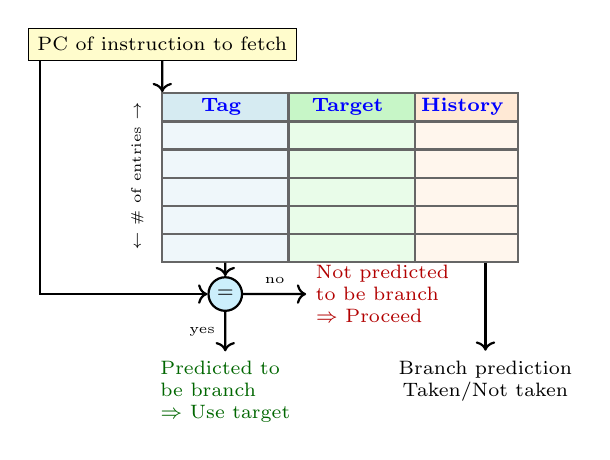
\begin{tikzpicture}[scale=0.8]
    % BTB table as matrix (lecture_06 style)
    \matrix[matrix of nodes,
            column sep=-\pgflinewidth,
            row sep=-\pgflinewidth,
            inner sep=0pt,
            anchor=north,
            nodes in empty cells,
            nodes={draw=black!60, line width=0.6pt, align=center, inner sep=2pt, font=\scriptsize,
                   minimum width=1.6cm, minimum height=0.35cm},
            ampersand replacement=\&
        ] (btb) {
        |[fill=lightblue!50, font=\scriptsize\bfseries]| \textcolor{myblue}{Tag} \& |[fill=lightgreen!50, font=\scriptsize\bfseries]| \textcolor{myblue}{Target} \& |[fill=peach!60, font=\scriptsize\bfseries, minimum width=1.3cm]| \textcolor{myblue}{History} \\
        |[fill=lightblue!20]| \phantom{0} \& |[fill=lightgreen!20]| \phantom{0} \& |[fill=peach!25, minimum width=1.3cm]| \phantom{0} \\
        |[fill=lightblue!20]| \phantom{0} \& |[fill=lightgreen!20]| \phantom{0} \& |[fill=peach!25, minimum width=1.3cm]| \phantom{0} \\
        |[fill=lightblue!20]| \phantom{0} \& |[fill=lightgreen!20]| \phantom{0} \& |[fill=peach!25, minimum width=1.3cm]| \phantom{0} \\
        |[fill=lightblue!20]| \phantom{0} \& |[fill=lightgreen!20]| \phantom{0} \& |[fill=peach!25, minimum width=1.3cm]| \phantom{0} \\
        |[fill=lightblue!20]| \phantom{0} \& |[fill=lightgreen!20]| \phantom{0} \& |[fill=peach!25, minimum width=1.3cm]| \phantom{0} \\
    };

    \node[draw, rectangle, above=4mm of btb-1-1.north, xshift=-8mm, font=\scriptsize, fill=yellow!20] (pc) {PC of instruction to fetch};

    % BTB label positioned relative to matrix left
    \node[rotate=90, left=5mm of btb.north west, font=\tiny, anchor=north east] {$\leftarrow$ \# of entries $\rightarrow$};

    % Comparator positioned relative to first column bottom
    \node[circle, draw, thick, inner sep=2pt, font=\scriptsize, fill=cyan!20] (comp) at ($ (btb-6-1.south) + (0, -0.5) $) {=};

    % Arrows using relative positioning
    \draw[->, thick] (pc) -- (btb-1-1.north -| pc);
    \draw[->, thick] ([xshift=2mm]pc.south west) |- (comp.west);
    \draw[->, thick] (btb-6-1.south) -- (comp);

    \node[right=8mm of comp, font=\scriptsize, align=left, text=red!70!black] (no) {Not predicted\\to be branch\\$\Rightarrow$ Proceed};

    % Output logic positioned relative to comparator
    \draw[->, thick] (comp.east) -- node[above, font=\tiny]{no} (no);

    \node[below=5mm of comp, font=\scriptsize, align=left, text=mygreen!80!black] (yes) {Predicted to\\be branch\\$\Rightarrow$ Use target};
    \draw[->, thick] (comp.south) -- node[left, font=\tiny]{yes} (yes);

    % Prediction output from third column
    \draw[->, thick] ([xshift=3mm]btb-6-3.south) -- ++(0, -14mm) node[below, align=center, font=\scriptsize] {Branch prediction\\Taken/Not taken};
\end{tikzpicture}
}

\begin{document}

\frame{\titlepage}




%% Slide: A Basic Processor
\begin{frame}{A Basic Processor}
\begin{center}
\scalebox{0.58}{
\begin{circuitikz}[
    % Component styles (same as Pipelined CPU but without pipeline_reg)
    component/.style={draw, thick, minimum height=0.8cm},
    stage_label/.style={draw, thick, fill=blue!60, text=white, font=\bfseries, minimum width=1.2cm, minimum height=0.5cm, text depth=0.25ex},
    imem_block/.style={muxdemux, muxdemux def={Lh=3, NL=3, Rh=3, NR=3, w=3.6, square pins=1},
                        external pins width=0, align=center, text depth=3ex, fill=yellow!20},
    regfile/.style={muxdemux, muxdemux def={Lh=4, NL=4, Rh=4, NR=2, w=2.8, square pins=1},
                    external pins width=0, fill=red!20, align=center},
    alu_style/.style={muxdemux, muxdemux def={Lh=2.6, Rh=1.5, NL=2, NR=5, NT=1, w=1.3, inset w=0.5, inset Lh=2, inset Rh=0, square pins=1},
                     external pins width=0, fill=green!20, font=\scriptsize},
    adder/.style={muxdemux, muxdemux def={Lh=1.2, NL=2, Rh=0.6, NR=1, w=1, inset w=0.3, inset Lh=0.6, inset Rh=0, square pins=1},
                     external pins width=0, fill=blue!20, font=\scriptsize},
    mux2/.style={muxdemux, muxdemux def={Lh=1.6, Rh=0.8, NL=2, NR=1, NT=1, w=0.8},
                 external pins width=0, fill=green!30},
    pcsrc_mux/.style={muxdemux, muxdemux def={Lh=0.8, Rh=1.6, NL=1, NR=2, NT=1, w=0.8},
                 external pins width=0, fill=blue!20},
    arrow/.style={->, >=stealth, thick},
    data_path/.style={arrow, black},
    data_connector/.style={circle, fill, inner sep=1.2pt},
    control_label/.style={font=\footnotesize, text=orange!80!black, align=center},
    node distance=5mm and 5mm,
]

% First pass: place invisible nodes to get coordinates
% IF Stage Components
\node[component, fill=blue!30, minimum width=0.8cm] (PC) {IP};
\node[imem_block, right=of PC, anchor=blpin 2] (IMem) {Inst.\\Cache};
\node[adder, above=2mm of IMem.north, anchor=south] (PCadder) {+};
\node[pcsrc_mux, anchor=south] (PCSrcMux) at ([yshift=20mm]IMem.north west) {};
\node[font=\scriptsize, left=5mm of PCadder.blpin 2] (four) {4};

% ID Stage Components
\node[regfile, right=25mm of IMem] (RegFile) {\rotatebox{90}{Register File}};

% Decode unit (control signal generator)
\node[ellipse, draw, thick, fill=orange!30, minimum width=1.2cm, minimum height=0.6cm, inner sep=0pt,
      font=\scriptsize] (Decode) at ([yshift=15mm,xshift=-8mm]RegFile.north) {decode};

% Sign Extend unit
\node[ellipse, draw, thick, fill=green!30, minimum width=0.3cm, minimum height=0.2cm, inner sep=0pt,
      font=\tiny, below=2mm of RegFile.south] (SignExt) {\rotatebox{90}{Sign Ext.}};

% EX Stage Components - ALU and MUX for immediate selection
\node[alu_style, anchor=blpin 1] (ALU) at ([xshift=4cm]RegFile.rpin 1) {};
\node[mux2, anchor=rpin 1] (ALUMux) at ([xshift=-6mm]ALU.lpin 2) {};
\node[font=\scriptsize, below right=-2mm of ALU.blpin 1] {\rotatebox{-45}{ALU}};

% Target calculation adder
\node[adder, anchor=lpin 1] (TargetAdder) at ([xshift=-5mm]ALU.west |- PCadder.rpin 1) {+};

% MEM Stage Components
\node[muxdemux, muxdemux def={Lh=4.1, NL=10, Rh=4.1, NR=10, w=2.8, square pins=1},
      external pins width=0, align=center, text depth=6.5ex, fill=yellow!20, anchor=lpin 5] (DMem) at ([xshift=1.5cm]ALU.brpin 4) {Data\\Cache};

% WB Stage
\node[mux2, anchor=lpin 1] at ([xshift=15mm]DMem.rpin 5) (WBMux) {};

% Stage boundary X coordinates
\coordinate (IF_left) at ([xshift=-8mm]PC.west);
\coordinate (IF_right) at ([xshift=4mm]IMem.east);
\coordinate (ID_right) at ([xshift=8mm]RegFile.east);
\coordinate (EX_right) at ([xshift=5mm]ALU.east);
\coordinate (MEM_right) at ([xshift=5mm]DMem.east);
\coordinate (WB_right) at ([xshift=12mm]WBMux.east);

% Stage label Y coordinate
\coordinate (label_y) at ([yshift=37mm]IMem.north);

% Stage labels - centered in shaded areas (using path midway)
\path (IF_left) -- (IF_right) coordinate[midway] (IF_mid);
\path (IF_right) -- (ID_right) coordinate[midway] (ID_mid);
\path (ID_right) -- (EX_right) coordinate[midway] (EX_mid);
\path (EX_right) -- (MEM_right) coordinate[midway] (MEM_mid);
\path (MEM_right) -- (WB_right) coordinate[midway] (WB_mid);

\node[stage_label] (IF_label) at (IF_mid |- label_y) {Fetch};
\node[stage_label] (ID_label) at (ID_mid |- label_y) {Decode};
\node[stage_label] (EX_label) at (EX_mid |- label_y) {Execute};
\node[stage_label] (MEM_label) at (MEM_mid |- label_y) {Memory};
\node[stage_label] (WB_label) at (WB_mid |- label_y) {WB};

% Stage background shades (drawn behind using scopes)
\begin{scope}[on background layer]
    % Common Y coordinates for all stages
    \coordinate (stage_top) at ([yshift=3mm]IF_label.north);
    \coordinate (stage_bottom) at ([yshift=-8mm]SignExt.south);

    % IF stage shade
    \fill[blue!8] (IF_left |- stage_top) rectangle (IF_right |- stage_bottom);

    % ID stage shade
    \fill[green!8] (IF_right |- stage_top) rectangle (ID_right |- stage_bottom);

    % EX stage shade
    \fill[blue!8] (ID_right |- stage_top) rectangle (EX_right |- stage_bottom);

    % MEM stage shade
    \fill[green!8] (EX_right |- stage_top) rectangle (MEM_right |- stage_bottom);

    % WB stage shade
    \fill[blue!8] (MEM_right |- stage_top) rectangle (WB_right |- stage_bottom);
\end{scope}

% === Data paths ===
% MUX output to PC
\coordinate (IP_west_conn) at ([xshift=-5mm]PC.west);
\draw[data_path] (PCSrcMux.lpin 1) -| (IP_west_conn) -- (PC.west);
\draw[data_path] (PC.east) -- (IMem.blpin 2);

% PC to adder
\node[data_connector] (PC_conn) at ([xshift=3mm]PC.east) {};
\draw[data_path] (PC_conn) |- (PCadder.blpin 1);
\draw[data_path] (four.east) -- (PCadder.blpin 2);

% PC+4 back to mux and to target adder
\draw[data_path] (PCadder.brpin 1) -- ++(4mm,0) node[data_connector] (NextSeqConn) {} |- (PCSrcMux.rpin 2);
\draw[data_path] (NextSeqConn) -- ++(0,0) -| ([xshift=-5mm]TargetAdder.lpin 1) -- (TargetAdder.lpin 1);

% IMem to RegFile and Decode
\draw[data_path] (IMem.brpin 2) -- ++(1,0) node[data_connector] (InstJunction) {};
\draw[data_path] (InstJunction) |- (RegFile.blpin 1);
\draw[data_path] (InstJunction) |- (RegFile.blpin 2);

% Instruction to Decode
\draw[data_path] (InstJunction) |- (Decode.west);

% Control signals from Decode
\draw[data_path, orange!80!black] (Decode.east) -- (Decode -| WBMux.tpin 1) node[control_label, above=-1pt, pos=0.2] {Control signals};

% ALU source control
\coordinate (ctrl_alusrc) at (Decode -| ALUMux.tpin 1);
\node[data_connector, fill=orange!80!black] at (ctrl_alusrc) {};
\draw[->, >=stealth, thick, orange!80!black] (ctrl_alusrc) -- (ALUMux.tpin 1) node[control_label, pos=0.2, right] {ALU\\source};

% ALU Control
\coordinate (ctrl_aluctl) at (Decode -| ALU.tpin 1);
\node[data_connector, fill=orange!80!black] at (ctrl_aluctl) {};
\draw[->, >=stealth, thick, orange!80!black] (ctrl_aluctl) -- (ALU.tpin 1) node[control_label, pos=0.25, right] {ALU\\Control};

% Mem Rd/Wr
\coordinate (ctrl_mem) at (Decode -| DMem.north);
\node[data_connector, fill=orange!80!black] at (ctrl_mem) {};
\draw[->, >=stealth, thick, orange!80!black] (ctrl_mem) -- (DMem.north) node[control_label, pos=0.25, right] {Mem\\Rd/Wr};

% WB select
\coordinate (ctrl_wbsel) at (Decode -| WBMux.tpin 1);
\node[data_connector, fill=orange!80!black] at (ctrl_wbsel) {};
\draw[->, >=stealth, thick, orange!80!black] (ctrl_wbsel) -- (WBMux.tpin 1) node[control_label, pos=0.3, right] {WB\\select};

% RegFile to ALU
\draw[data_path] (RegFile.rpin 1) -- (ALU.lpin 1);
\coordinate (WriteDataJunction) at ([xshift=-3mm]ALUMux.lpin 1);
\draw[data_path] (RegFile.rpin 2 |- WriteDataJunction) -- (WriteDataJunction) node[data_connector] {} -- (ALUMux.blpin 1);

% Write data to DMem
\draw[data_path] (WriteDataJunction) |- (DMem.lpin 10);

% Sign Extend to ALUMux and Target Adder
\draw[data_path] (InstJunction) |- (SignExt.west);
\coordinate (ImmJunction) at ([xshift=-7mm]ALUMux.lpin 2);
\draw[data_path] (SignExt.east) -| (ImmJunction) -- (ALUMux.lpin 2);
\node[data_connector] at (ImmJunction) {};
\draw[data_path] (ImmJunction) |- (TargetAdder.lpin 2);

% Target Adder to PC mux
\draw[data_path] (TargetAdder.rpin 1) -- ++(5mm,0) |- (PCSrcMux.rpin 1);

% ALU to DMem (address)
\draw[data_path] (ALU.brpin 4) -- (DMem.lpin 5);

% DMem to WB Mux
\draw[data_path] (DMem.rpin 5) -- (WBMux.blpin 1);

% ALU result to WB Mux (bypass memory)
\node[data_connector] (ALUResConn) at ([xshift=5mm]ALU.brpin 4) {};
\draw[data_path] (ALUResConn) |- ([yshift=-5mm]DMem.south) -| ([xshift=-5mm]WBMux.lpin 2) -- (WBMux.lpin 2);

% WB Mux output to Register File write data
\coordinate (dst_y_level) at ([yshift=-5mm]SignExt.south);
\draw[data_path] (WBMux.rpin 1) -- ++(0.5,0) |- ([xshift=-3mm]RegFile.blpin 4 |- dst_y_level) -- ([xshift=-3mm]RegFile.blpin 4) -- (RegFile.blpin 4);

% Dst from instruction to RegFile
\draw[data_path] (InstJunction) |- (RegFile.blpin 3);

% Register File labels
\node[align=left, xshift=3mm, font=\tiny] at (RegFile.blpin 1) {src1};
\node[align=left, xshift=3mm, font=\tiny] at (RegFile.blpin 2) {src2};
\node[align=left, xshift=3mm, font=\tiny] at (RegFile.blpin 3) {dst};
\node[align=left, xshift=3mm, font=\tiny] at (RegFile.blpin 4) {data};
\node[align=right, xshift=-3mm, font=\tiny] at (RegFile.brpin 1) {src1\\data};
\node[align=right, xshift=-3mm, font=\tiny] at (RegFile.brpin 2) {src2\\data};

% Data Cache labels
\node[align=left, font=\tiny] at ([xshift=3mm,yshift=-1mm]DMem.lpin 5) {address};
\node[align=left, font=\tiny] at ([xshift=3mm, yshift=2mm]DMem.lpin 10) {data};
\node[align=right, font=\tiny] at ([xshift=-3mm,yshift=-2mm]DMem.rpin 5) {data};

\end{circuitikz}
}
\end{center}
\end{frame}

%% Slide: Pipelined Car Assembly - Combined with overlays
\begin{frame}{Pipelined Car Assembly}
    \centering
    \begin{tikzpicture}[
        stage/.style={draw, thick, minimum width=3cm, minimum height=2.4cm, align=center, font=\large\bfseries},
        ]

        % Time progress bar - changes with each overlay
        \draw[draw=black, thick] (-5, 4) rectangle (5, 4.4);
        \only<1>{\fill[fill=blue!40] (-5, 4) rectangle (-5, 4.4);}
        \only<2>{\fill[fill=blue!40] (-5, 4) rectangle (-3.57, 4.4);}
        \only<3>{\fill[fill=blue!40] (-5, 4) rectangle (-0.71, 4.4);}
        \only<4>{\fill[fill=blue!40] (-5, 4) rectangle (0.14, 4.4);}
        \only<5>{\fill[fill=blue!40] (-5, 4) rectangle (1.43, 4.4);}
        \only<6>{\fill[fill=blue!40] (-5, 4) rectangle (2.86, 4.4);}
        \only<7>{\fill[fill=blue!40] (-5, 4) rectangle (5, 4.4);}

        \only<1>{\node[right, font=\Large\bfseries] at (5.2, 4.2) {00:00};}
        \only<2>{\node[right, font=\Large\bfseries] at (5.2, 4.2) {01:00};}
        \only<3>{\node[right, font=\Large\bfseries] at (5.2, 4.2) {03:00};}
        \only<4>{\node[right, font=\Large\bfseries] at (5.2, 4.2) {04:00};}
        \only<5>{\node[right, font=\Large\bfseries] at (5.2, 4.2) {05:00};}
        \only<6>{\node[right, font=\Large\bfseries] at (5.2, 4.2) {06:00};}
        \only<7>{\node[right, font=\Large\bfseries] at (5.2, 4.2) {07:00};}

        % Three stages (always visible)
        \node[stage, fill=orange!40] (chassis) at (-4, 2) {
            
\includegraphics[width=1cm]{generated/noun-chassis-8091073.pdf}\\~
        };
        \node[font=\small, anchor=south] at (chassis.south) {chassis};
        \node[font=\small, anchor=north] at (chassis.south) {1 hour};

        \node[stage, fill=green!40, right=1cm of chassis] (engine) {
            
\includegraphics[width=1.2cm]{generated/noun-engine-8079892.pdf}\\~
        };
        \node[font=\small, anchor=south] at (engine.south) {engine};
        \node[font=\small, anchor=north] at (engine.south) {2 hours};

        \node[stage, fill=blue!40, right=1cm of engine] (finish) {
            
\includegraphics[width=1.2cm]{generated/noun-car-spray-5038977.pdf}\\~
        };
        \node[font=\small, anchor=south] at (finish.south) {finish};
        \node[font=\small, anchor=north] at (finish.south) {1 hour};

        % Overlay 1: 00:00 - Car 1 at chassis
        \only<1>{
            \node[below=0.8cm of chassis] (car1) {
                
\includegraphics[width=1.2cm]{generated/noun-car-4612699.pdf}
            };
            \node[below=0.05cm of car1, font=\small] {Car 1};
        }

        % Overlay 2: 01:00 - Car 2 at chassis, Car 1 at engine
        \only<2>{
            \node[below=0.8cm of chassis] (car2) {
                \includegraphics[width=1.2cm]{generated/noun-car-2302591.pdf}
            };
            \node[below=0.05cm of car2, font=\small] (car2title) {Car 2};

            \node at (car2 -| engine) (car1) {
                
\includegraphics[width=1.2cm]{generated/noun-car-4612699.pdf}
            };
            \node[font=\small] at (car2title -| car1) {Car 1};
        }

        % Overlay 3: 03:00 - Car 3 at chassis, Car 2 at engine, Car 1 at finish
        \only<3>{
            \node[below=0.8cm of chassis] (car3) {
                
\includegraphics[width=1.2cm]{generated/noun-car-24929.pdf}
            };
            \node[below=0.05cm of car3, font=\small] (car3title) {Car 3};

            \node at (car3 -| engine) (car2) {
                \includegraphics[width=1.2cm]{generated/noun-car-2302591.pdf}
            };
            \node[font=\small] at (car3title -| car2) {Car 2};

            \node at (car3 -| finish) (car1) {
                
\includegraphics[width=1.2cm]{generated/noun-car-4612699.pdf}
            };
            \node[font=\small] at (car3title -| car1) {Car 1};

            \node[align=center, font=\small] at (0, -2) {
                Car 2 waited an hour after finishing station 1\\
                for Car 1 to finish station 2
            };
        }

        % Overlay 4: 04:00 - Car 3 at chassis, Car 2 at engine, Car 1 done
        \only<4>{
            \node[below=0.8cm of chassis] (car3) {
                
\includegraphics[width=1.2cm]{generated/noun-car-24929.pdf}
            };
            \node[below=0.05cm of car3, font=\small] (car3title) {Car 3};

            \node at (car3 -| engine) (car2) {
                \includegraphics[width=1.2cm]{generated/noun-car-2302591.pdf}
            };
            \node[font=\small] at (car3title -| car2) {Car 2};

            % Clock icon next to Car 2
            \node[right=0.05cm of car2] (clock2) {
                \includegraphics[width=1.25cm]{figures/noun-clock-2310543.png}
            };

            \node at (6, -1) (car1) {
                
\includegraphics[width=1.2cm]{generated/noun-car-4612699.pdf}
            };
            \node[below=0.05cm of car1, font=\small] {Car 1};

            \node[align=center, font=\normalsize] at (0, -2) {
                \textbf{First car done after 4 hours}\\
                Car 2 still needs another hour to finish engine work
            };
        }

        % Overlay 5: 05:00 - Car 4 at chassis, Car 3 at engine, Car 2 at finish
        \only<5>{
            \node[below=0.8cm of chassis] (car4) {
                
\includegraphics[width=1.2cm]{generated/noun-car-2502122.pdf}
            };
            \node[below=0.05cm of car4, font=\small] (car4title) {Car 4};

            \node at (car4 -| engine) (car3) {
                
\includegraphics[width=1.2cm]{generated/noun-car-24929.pdf}
            };
            \node[font=\small] at (car4title -| car3) {Car 3};

            \node at (car4 -| finish) (car2) {
                \includegraphics[width=1.2cm]{generated/noun-car-2302591.pdf}
            };
            \node[font=\small] at (car4title -| car2) {Car 2};
        }

        % Overlay 6: 06:00 - Car 4 at chassis, Car 3 at engine, Car 2 done
        \only<6>{
            \node[below=0.8cm of chassis] (car4) {
                
\includegraphics[width=1.2cm]{generated/noun-car-2502122.pdf}
            };
            \node[below=0.05cm of car4, font=\small] (car4title) {Car 4};

            \node at (car4 -| engine) (car3) {
                
\includegraphics[width=1.2cm]{generated/noun-car-24929.pdf}
            };
            \node[font=\small] at (car4title -| car3) {Car 3};

            % Clock icon next to Car 3
            \node[right=0.05cm of car3] (clock3) {
                \includegraphics[width=1.25cm]{figures/noun-clock-2310543.png}
            };

            \node at (6, -1) (car2) {
                \includegraphics[width=1.2cm]{generated/noun-car-2302591.pdf}
            };
            \node[below=0.05cm of car2, font=\small] {Car 2};

            \node[align=center, font=\small] at (0, -2) {
                Car 2 completes at 06:00\\
                (2 hours after Car 1)
            };
        }

        % Overlay 7: 07:00 - Car 5 at chassis, Car 4 at engine, Car 3 at finish
        \only<7>{
            \node[below=0.8cm of chassis] (car5) {
                
\includegraphics[width=1.2cm]{generated/noun-car-25465.pdf}
            };
            \node[below=0.05cm of car5, font=\small] (car5title) {Car 5};

            \node at (car5 -| engine) (car4) {
                
\includegraphics[width=1.2cm]{generated/noun-car-2502122.pdf}
            };
            \node[font=\small] at (car5title -| car4) {Car 4};

            \node at (car5 -| finish) (car3) {
                
\includegraphics[width=1.2cm]{generated/noun-car-24929.pdf}
            };
            \node[font=\small] at (car5title -| car3) {Car 3};

            \node[align=left, font=\normalsize] at (0, -2) {
                \textbf{Pipeline latency is 4 hours}\\[1mm]
                \textbf{Pipeline throughput is one car every 2 hours}
            };
        }
    \end{tikzpicture}
\end{frame}

%% Slide: Pipelined Car Assembly
\begin{frame}{Pipelining Instructions}
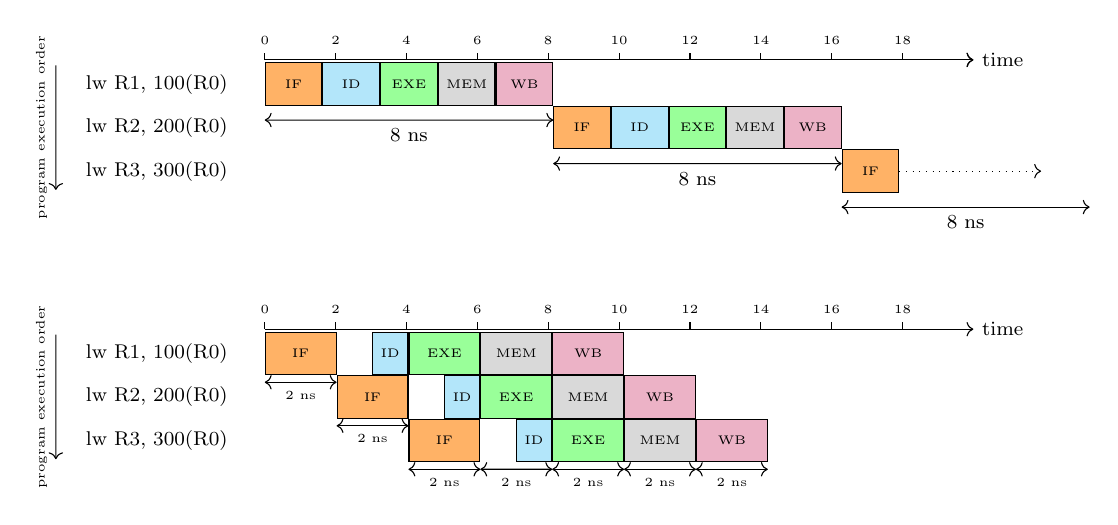
\begin{tikzpicture}[scale=0.9, transform shape,
    stage/.style={draw, minimum height=6mm, minimum width=8mm, font=\tiny, align=center, inner sep=1pt},
    fetch/.style={stage, fill=orange!60},
    reg/.style={stage, fill=cyan!30},
    alu/.style={stage, fill=green!40},
    mem/.style={stage, fill=gray!30},
    wb/.style={stage, fill=purple!30},
    pfetch/.style={stage, fill=orange!60, minimum width=10mm},
    preg/.style={stage, fill=cyan!30, minimum width=5mm},
    palu/.style={stage, fill=green!40, minimum width=10mm},
    pmem/.style={stage, fill=gray!30, minimum width=10mm},
    pwb/.style={stage, fill=purple!30, minimum width=10mm},]


% First pipeline diagram (non-pipelined)

% Time axis for first diagram with ticks above
\coordinate (timeline_start) at (1, 1.5);
\coordinate (timeline_end) at (11, 1.5);
\draw[->] (timeline_start) -- (timeline_end);
\draw[->] (timeline_start) -- (timeline_end)
  node[pos=1, right]{\footnotesize time};

\foreach \x/\t in {1/0, 2/2, 3/4, 4/6, 5/8, 6/10, 7/12, 8/14, 9/16, 10/18} {
    \draw (\x, 1.5) -- (\x, 1.6);  % tick marks
    \node[above] (t1-\t) at (\x, 1.6) {\tiny \t};
}

% First instruction row
\node[fetch, anchor=north west] (f1) at ([yshift=-1]timeline_start) {IF};
\node[anchor=east] (f1ins) at ([xshift=-4mm]f1.west) {\footnotesize lw R1, 100(R0)};
\node[reg, anchor=west] (r1a) at (f1.east) {ID};
\node[alu, anchor=west] (a1) at (r1a.east) {EXE};
\node[mem, anchor=west] (m1) at (a1.east) {MEM};
\node[wb, anchor=west] (r1b) at (m1.east) {WB};

% Second instruction row  
\node[fetch, anchor=north west] (f2) at (r1b.south east) {IF};
\node (f2ins) at (f1ins |- f2) {\footnotesize lw R2, 200(R0)};
\node[reg, anchor=west] (r2a) at (f2.east) {ID};
\node[alu, anchor=west] (a2) at (r2a.east) {EXE};
\node[mem, anchor=west] (m2) at (a2.east) {MEM};
\node[wb, anchor=west] (r2b) at (m2.east) {WB};

% Third instruction row
\node[fetch, anchor=north west] (f3) at (r2b.south east) {IF};
\node (f3ins) at (f1ins |- f3) {\footnotesize lw R3, 300(R0)};
\draw[dotted, ->] (f3.east) -- ++(2, 0);

% Timing annotations using relative positioning
\draw[<->] ([yshift=-2mm]f1.south west) -- node[below] {\footnotesize 8 ns} ([yshift=-2mm]r1b.south east);

\draw[<->] ([yshift=-2mm]f2.south west) -- node[below] {\footnotesize 8 ns} ([yshift=-2mm]r2b.south east);

\draw[<->] ([yshift=-2mm]f3.south west) -- node[below] {\footnotesize 8 ns} ++(3.5, 0);

% Vertical arrow for execution order - relative to instructions
\draw[->] 
  ([xshift=-3mm]f1ins.north west)
    -- node[rotate=90, anchor=south]{\tiny program execution order}
  ([xshift=-3mm]f3ins.south west);


% Second pipeline diagram (pipelined) - moved higher

% Time axis for second diagram
\coordinate (ptimeline_start) at (1, -2.3);
\coordinate (ptimeline_end) at (11, -2.3);

\draw[->] (ptimeline_start) -- (ptimeline_end)
  node[pos=1, right]{\footnotesize time};
\foreach \x/\t in {1/0, 2/2, 3/4, 4/6, 5/8, 6/10, 7/12, 8/14, 9/16, 10/18} {
    \draw (\x, -2.3) -- (\x, -2.2);  % tick marks
    \node[above] (t2-\t) at (\x, -2.2) {\tiny \t};
}

% First instruction (pipelined)
\node[pfetch, anchor=north west] (pf1) at ([yshift=-1]ptimeline_start) {IF};
\node[anchor=east] (pf1ins) at ([xshift=-4mm]pf1.west) {\footnotesize lw R1, 100(R0)};
\node[preg, anchor=west] (pr1a) at ([xshift=5mm]pf1.east) {ID};
\node[palu, anchor=west] (pa1) at (pr1a.east) {EXE};
\node[pmem, anchor=west] (pm1) at (pa1.east) {MEM};
\node[pwb, anchor=west] (pr1b) at (pm1.east) {WB};

% Second instruction (pipelined - starts after first Inst Fetch)
\node[pfetch, anchor=north west] (pf2) at (pf1.south east) {IF};
\node (pf2ins) at (pf1ins |- pf2) {\footnotesize lw R2, 200(R0)};
\node[preg, anchor=west] (pr2a) at ([xshift=5mm]pf2.east) {ID};
\node[palu, anchor=west] (pa2) at (pr2a.east) {EXE};
\node[pmem, anchor=west] (pm2) at (pa2.east) {MEM};
\node[pwb, anchor=west] (pr2b) at (pm2.east) {WB};

% Third instruction (pipelined - starts after second Inst Fetch)
\node[pfetch, anchor=north west] (pf3) at (pf2.south east) {IF};
\node (pf3ins) at (pf1ins |- pf3) {\footnotesize lw R3, 300(R0)};
\node[preg, anchor=west] (pr3a) at ([xshift=5mm]pf3.east) {ID};
\node[palu, anchor=west] (pa3) at (pr3a.east) {EXE};
\node[pmem, anchor=west] (pm3) at (pa3.east) {MEM};
\node[pwb, anchor=west] (pr3b) at (pm3.east) {WB};

% Timing annotations for pipeline stages
\draw[<->] ([yshift=-1mm]pf1.south west) -- node[below, font=\tiny] {2 ns} ([yshift=-1mm]pf1.south east);

\draw[<->] ([yshift=-1mm]pf2.south west) -- node[below, font=\tiny] {2 ns} ([yshift=-1mm]pf2.south east);

\draw[<->] ([yshift=-1mm]pf3.south west) -- node[below, font=\tiny] {2 ns} ([yshift=-1mm]pf3.south east);

\draw[<->] ([yshift=-1mm]pf3.south east) -- node[below, font=\tiny] {2 ns} ([yshift=-1mm]pa3.south west);

\draw[<->] ([yshift=-1mm]pa3.south west) -- node[below, font=\tiny] {2 ns} ([yshift=-1mm]pa3.south east);

\draw[<->] ([yshift=-1mm]pm3.south west) -- node[below, font=\tiny] {2 ns} ([yshift=-1mm]pm3.south east);

\draw[<->] ([yshift=-1mm]pr3b.south west) -- node[below, font=\tiny] {2 ns} ([yshift=-1mm]pr3b.south east);

% Vertical arrow for execution order - relative to instructions
\draw[->] 
  ([xshift=-3mm]pf1ins.north west)
    -- node[rotate=90, anchor=south]{\tiny program execution order}
  ([xshift=-3mm]pf3ins.south west);

\end{tikzpicture}

\vspace{0.2cm}
\centering
\large Ideal speedup is number of stages in the pipeline. Do we achieve this?
\end{frame}


%% Slide: Pipelined CPU
\begin{frame}{Pipelined CPU}
\begin{center}
\scalebox{0.58}{
\begin{circuitikz}[
    % Component styles
    component/.style={draw, thick, minimum height=0.8cm},
    pipeline_reg/.style={draw, thick, fill=yellow!40, minimum width=6mm, minimum height=6.2cm},
    stage_label/.style={draw, thick, fill=blue!60, text=white, font=\bfseries, minimum width=1.2cm, minimum height=0.5cm, text depth=0.25ex},
    imem_block/.style={muxdemux, muxdemux def={Lh=3, NL=3, Rh=3, NR=3, w=3.6, square pins=1},
                        external pins width=0, align=center, text depth=3ex, fill=yellow!20},
    regfile/.style={muxdemux, muxdemux def={Lh=4, NL=4, Rh=4, NR=2, w=2.8, square pins=1},
                    external pins width=0, fill=red!20, align=center},
    alu_style/.style={muxdemux, muxdemux def={Lh=2.6, Rh=1.5, NL=2, NR=5, NT=1, w=1.3, inset w=0.5, inset Lh=2, inset Rh=0, square pins=1},
                     external pins width=0, fill=green!20, font=\scriptsize},
    adder/.style={muxdemux, muxdemux def={Lh=1.2, NL=2, Rh=0.6, NR=1, w=1, inset w=0.3, inset Lh=0.6, inset Rh=0, square pins=1},
                     external pins width=0, fill=blue!20, font=\scriptsize},
    mux2/.style={muxdemux, muxdemux def={Lh=1.6, Rh=0.8, NL=2, NR=1, NT=1, w=0.8},
                 external pins width=0, fill=green!30},
    pcsrc_mux/.style={muxdemux, muxdemux def={Lh=0.8, Rh=1.6, NL=1, NR=2, NT=1, w=0.8},
                 external pins width=0, fill=blue!20},
    arrow/.style={->, >=stealth, thick},
    data_path/.style={arrow, black},
    line_label/.style={above, inner sep=1pt, font=\footnotesize},
    data_connector/.style={circle, fill, inner sep=1.2pt},
    data_latch/.style={draw, thick, fill=cyan!20, minimum width=6mm, minimum height=0.3cm, inner sep=1pt, font=\tiny},
    control_label/.style={font=\footnotesize, text=orange!80!black, align=center},
    node distance=5mm and 5mm,
]

% IF Stage Components
\node[component, fill=blue!30, minimum width=0.8cm] (PC) {IP};
\node[imem_block, right=of PC, anchor=blpin 2] (IMem) {Inst.\\Cache};
\node[adder, above=2mm of IMem.north, anchor=south] (PCadder) {+};
\node[pcsrc_mux, anchor=south] (PCSrcMux) at ([yshift=20mm]IMem.north west) {};
\node[font=\scriptsize, left=5mm of PCadder.blpin 2] (four) {4};

% Pipeline register IF/ID
\node[pipeline_reg, right=8mm of IMem.brpin 2] (IFID) {};
\node[data_latch, minimum height=2cm] (instruction) at (IMem.rpin 2 -| IFID) {\rotatebox{90}{Instruction}};

% ID Stage Components
\node[regfile, right=15mm of IFID] (RegFile) {\rotatebox{90}{Register File}};

% Decode unit (control signal generator)
\node[ellipse, draw, thick, fill=orange!30, minimum width=1.2cm, minimum height=0.6cm, inner sep=0pt,
      font=\scriptsize] (Decode) at ([yshift=15mm,xshift=-8mm]RegFile.north) {decode};

% Sign Extend unit
\node[ellipse, draw, thick, fill=green!30, minimum width=0.3cm, minimum height=0.2cm, inner sep=0pt,
      font=\tiny, below=2mm of RegFile.south] (SignExt) {\rotatebox{90}{Sign Ext.}};

% Pipeline register ID/EX
\node[pipeline_reg, right=8mm of RegFile.east |- IFID] (IDEX) {};

% EX Stage Components - ALU and MUX for immediate selection
\node[alu_style, anchor=blpin 1] (ALU) at ([xshift=2.5cm]RegFile.brpin 1 -| IDEX.east) {};
\node[mux2, anchor=rpin 1] (ALUMux) at ([xshift=-6mm]ALU.lpin 2) {};
\node[font=\scriptsize, below right=-2mm of ALU.blpin 1] {\rotatebox{-45}{ALU}};

% Target calculation adder
\node[adder, anchor=lpin 1] (TargetAdder) at ([xshift=-5mm]ALU.west |- PCadder.rpin 1) {+};


% Pipeline register EX/MEM
\node[pipeline_reg, right=12mm of ALU.east |- IDEX] (EXMEM) {};

% MEM Stage Components
\node[muxdemux, muxdemux def={Lh=4.1, NL=10, Rh=4.1, NR=10, w=2.8, square pins=1},
      external pins width=0, align=center, text depth=6.5ex, fill=yellow!20, anchor=lpin 5] (DMem) at ([xshift=1cm]ALU.brpin 4 -| EXMEM.east) {Data\\Cache};


% Pipeline register MEM/WB
\node[pipeline_reg, right=8mm of DMem.east |- EXMEM] (MEMWB) {};

% WB Stage
\node[mux2, anchor=lpin 1] at ([xshift=8mm]MEMWB.east |- DMem.rpin 5) (WBMux) {};


% Stage labels
\node[stage_label] (IF_label) at ([yshift=37mm]IMem.north) {Fetch};
\node[stage_label] (ID_label) at (IF_label -| RegFile) {Decode};
\node[stage_label] (EX_label) at (IF_label -| ALU) {Execute};
\node[stage_label] (MEM_label) at (IF_label -| DMem) {Memory};
\node[stage_label] (WB_label) at (IF_label -| WBMux) {WB};

% === Routing coordinates for pipeline signal propagation ===
% Next sequential address coordinates
\coordinate (fetch_out_next_seq) at (PCadder.brpin 1 -| IFID.west);
\coordinate (decode_in_next_seq) at (IFID.east |- fetch_out_next_seq);
\coordinate (decode_out_next_seq) at (IDEX.west |- fetch_out_next_seq);
\coordinate (execute_in_next_seq) at (IDEX.east |- fetch_out_next_seq);

% Target register (dst) coordinates - unified Y level at 5mm below SignExt.south
\coordinate (dst_y_level) at ([yshift=-5mm]SignExt.south);
\coordinate (dst_idex_in) at (IDEX.west |- dst_y_level);
\coordinate (dst_idex_out) at (IDEX.east |- dst_y_level);
\coordinate (dst_exmem_in) at (EXMEM.west |- dst_y_level);
\coordinate (dst_exmem_out) at (EXMEM.east |- dst_y_level);
\coordinate (dst_memwb_in) at (MEMWB.west |- dst_y_level);
\coordinate (dst_memwb_out) at (MEMWB.east |- dst_y_level);

% === Data paths ===
% MUX output to PC
\coordinate (IP_west_conn) at ([xshift=-5mm]PC.west);
\draw[data_path] (PCSrcMux.lpin 1) -| (IP_west_conn) -- (PC.west);
\draw[data_path] (PC.east) -- (IMem.blpin 2);

% PC to adder
\node[data_connector] (PC_conn) at ([xshift=3mm]PC.east) {};
\draw[data_path] (PC_conn) |- (PCadder.blpin 1);
\draw[data_path] (four.east) -- (PCadder.blpin 2);

% === Next sequential address ===
\draw[data_path] (PCadder.brpin 1) -- ++(4mm,0) node[data_connector] (NextSeqConn) {} -- ++(0.1,0) |- (fetch_out_next_seq);
\draw[data_path] (NextSeqConn) |- (PCSrcMux.rpin 2);
\draw[data_path] (decode_in_next_seq) -- (decode_out_next_seq);
\draw[data_path] (execute_in_next_seq) |- (TargetAdder.lpin 1);

% IMem to IF/ID
\draw[data_path] (IMem.brpin 2) -- (IFID.west |- IMem.brpin 2);

% Instruction to Decode (straight line at same Y)
\draw[data_path] (IFID.east |- Decode) -- (Decode.west);

% === Control signal paths (propagate through pipeline latches) ===
% Control signals Y coordinate (same as Decode)
\coordinate (ctrl_idex_in) at (IDEX.west |- Decode);
\coordinate (ctrl_idex_out) at (IDEX.east |- Decode);
\coordinate (ctrl_exmem_in) at (EXMEM.west |- Decode);
\coordinate (ctrl_exmem_out) at (EXMEM.east |- Decode);
\coordinate (ctrl_memwb_in) at (MEMWB.west |- Decode);
\coordinate (ctrl_memwb_out) at (MEMWB.east |- Decode);

% Control signal lines between latches
\draw[data_path, orange!80!black] (Decode.east) -- (ctrl_idex_in) node[control_label, above=-2pt, midway] {Control\\signals};
\draw[data_path, orange!80!black] (ctrl_idex_out) -- (ctrl_exmem_in);
\draw[data_path, orange!80!black] (ctrl_exmem_out) -- (ctrl_memwb_in);

% Control signal arrows to components with data-connectors
% ALU source (vertical from control line to ALUMux top pin)
\coordinate (ctrl_alusrc) at (Decode -| ALUMux.tpin 1);
\node[data_connector, fill=orange!80!black] at (ctrl_alusrc) {};
\draw[->, >=stealth, thick, orange!80!black] (ctrl_alusrc) -- (ALUMux.tpin 1) node[control_label, pos=0.2, right] {ALU\\source};

% ALU Control (vertical from control line to ALU top pin)
\coordinate (ctrl_aluctl) at (Decode -| ALU.tpin 1);
\node[data_connector, fill=orange!80!black] at (ctrl_aluctl) {};
\draw[->, >=stealth, thick, orange!80!black] (ctrl_aluctl) -- (ALU.tpin 1) node[control_label, pos=0.25, right] {ALU\\Control};

% Mem Rd/Wr (vertical from control line to DMem top)
\coordinate (ctrl_mem) at (Decode -| DMem.north);
\node[data_connector, fill=orange!80!black] at (ctrl_mem) {};
\draw[->, >=stealth, thick, orange!80!black] (ctrl_mem) -- (DMem.north) node[control_label, pos=0.25, right] {Mem\\Rd/Wr};

% WB select (from control line at MEMWB east to WBMux top pin)
\draw[->, >=stealth, thick, orange!80!black] (ctrl_memwb_out) -| (WBMux.tpin 1) node[control_label, pos=0.55, right] {WB\\select};

% IF/ID to RegFile
\draw[data_path] (IFID.east |- RegFile.lpin 1) -- (RegFile.blpin 1);
\draw[data_path] (IFID.east |- RegFile.lpin 2) -- (RegFile.blpin 2);

% RegFile to ID/EX
\draw[data_path] (RegFile.brpin 1) -- (IDEX.west |- RegFile.brpin 1);
\draw[data_path] (RegFile.brpin 2) -- (IDEX.west |- RegFile.brpin 2);

% IF/ID to Sign Extend
\draw[data_path] (IFID.east |- SignExt) -- (SignExt.west);
% Sign Extend to ID/EX
\draw[data_path] (SignExt.east) -- (IDEX.west |- SignExt);

% Target register (dst) path
\node[font=\scriptsize, below=1mm of SignExt] {dst};
\draw[data_path] ([yshift=4mm]instruction.south east) -- ++(0.5,0) |- (dst_idex_in);

% ID/EX to ALU (top input direct, bottom through MUX)
\draw[data_path] (IDEX.east |- ALU.blpin 1) -- (ALU.blpin 1);
\coordinate (WriteDataJunction) at ([xshift=-3mm]ALUMux.lpin 1);
\draw[data_path] (IDEX.east |- ALUMux.lpin 1) -- (WriteDataJunction) node[data_connector] {} -- (ALUMux.blpin 1);
\draw[data_path] (WriteDataJunction) |- (EXMEM.west |- DMem.lpin 10);
\draw[data_path] (EXMEM.east |- DMem.lpin 10) -- (DMem.lpin 10);
\draw[data_path] (ALUMux.rpin 1) -- (ALU.blpin 2);

% SignExt through ID/EX to ALUMux and Target Adder
\coordinate (ImmJunction) at ([xshift=-7mm]ALUMux.lpin 2);
\draw[data_path] (SignExt -| IDEX.east) -| (ImmJunction) -- (ALUMux.lpin 2);
\node[data_connector] at (ImmJunction) {};
\draw[data_path] (ImmJunction) |- (TargetAdder.lpin 2);

% Target Adder to EX/MEM buffer
\coordinate (calc_target_exmem) at (TargetAdder.rpin 1 -| EXMEM.west);
\draw[data_path] (TargetAdder.brpin 1) -- (calc_target_exmem);

% ALU output to EX/MEM buffer (result only, no zero)
\coordinate (exmem_alu_result) at (ALU.brpin 4 -| EXMEM.west);
\draw[data_path] (ALU.brpin 4) -- (exmem_alu_result);

% EX/MEM to DMem (addr)
\draw[data_path] (EXMEM.east |- DMem.lpin 5) -- (DMem.lpin 5);

% DMem to MEM/WB (read data)
\draw[data_path] (DMem.rpin 5) -- (MEMWB.west |- DMem.rpin 5);

% Dst register propagation through pipeline
\draw[data_path] (dst_idex_out) -- (dst_exmem_in);
\draw[data_path] (dst_exmem_out) -- (dst_memwb_in);
\draw[data_path] (dst_memwb_out) -- ++(0.5,0) |- ([yshift=-5mm,xshift=-6mm]RegFile.west |- IDEX.south) |- (RegFile.blpin 3);

% MEM/WB to WB Mux
\draw[data_path] (MEMWB.east |- WBMux.lpin 1) -- (WBMux.blpin 1);

% Address path from DMem to WB Mux
\coordinate (AddrWB) at ([yshift=-3mm]DMem.south -| MEMWB.west);
\node[data_connector] (AddrConn) at ([xshift=-5mm]DMem.lpin 5) {};
\draw[data_path] (AddrConn) |- (AddrWB);
\draw[data_path] (AddrWB -| MEMWB.east) -- ++(0.5,0) |- (WBMux.lpin 2);

% WB Mux output to Register File write data
\draw[data_path] (WBMux.rpin 1) -- ++(0.5,0) |- ([xshift=-4mm,yshift=-8mm]IDEX.south -| RegFile.lpin 4) |- (RegFile.blpin 4);

% === Branch target path (from calc target back to PC mux) ===
\coordinate (calc_target_mem_out) at (calc_target_exmem -| EXMEM.east);
\draw[data_path] (calc_target_mem_out) -- ++(0.5,0) |- (PCSrcMux.rpin 1);

% Register File labels
\node[align=left, xshift=3mm, font=\tiny] at (RegFile.blpin 1) {src1};
\node[align=left, xshift=3mm, font=\tiny] at (RegFile.blpin 2) {src2};
\node[align=left, xshift=3mm, font=\tiny] at (RegFile.blpin 3) {dst};
\node[align=left, xshift=3mm, font=\tiny] at (RegFile.blpin 4) {data};
\node[align=right, xshift=-3mm, font=\tiny] at (RegFile.brpin 1) {src1\\data};
\node[align=right, xshift=-3mm, font=\tiny] at (RegFile.brpin 2) {src2\\data};

% Data Cache labels
\node[align=left, font=\tiny] at ([xshift=3mm,yshift=-1mm]DMem.lpin 5) {address};
\node[align=left, font=\tiny] at ([xshift=3mm, yshift=2mm]DMem.lpin 10) {data};
\node[align=right, font=\tiny] at ([xshift=-3mm,yshift=-2mm]DMem.rpin 5) {data};

\end{circuitikz}
}
\end{center}
\end{frame}

%% Slide: Structural Hazard
\begin{frame}{Structural Hazard}
    \textbf{Structural Hazard:} Different instructions using the same resource at the same time
    \vspace{1cm}
    
    \begin{columns}
        \column{0.45\textwidth}
        \textbf{Register File Contention:}
        \begin{itemize}
            \item Read during ID (stage 2)
            \item Write during WB (stage 5)
            \item Solution: 2 read ports, 1 write port
        \end{itemize}
        
        \vspace{0.3cm}
        \centering
        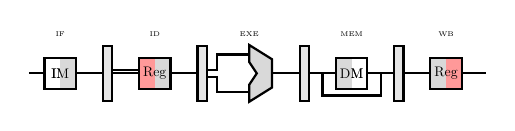
\begin{tikzpicture}[scale=0.5, transform shape]
            % Define styles
            \tikzstyle{block} = [rectangle, draw, thick, minimum width=0.8cm, minimum height=0.8cm, inner sep=2pt]
            \tikzstyle{latch} = [rectangle, draw, thick, minimum width=0.12cm, minimum height=1.4cm, fill=gray!20]
            \tikzstyle{line} = [draw, thick]
            
            % Stage labels
            \node[above] at (0,0.8) {\tiny IF};
            \node[above] at (2.4,0.8) {\tiny ID};
            \node[above] at (4.8,0.8) {\tiny EXE};
            \node[above] at (7.4,0.8) {\tiny MEM};
            \node[above] at (9.8,0.8) {\tiny WB};
            
            % Single pipeline row components
            \node[block, fill=white] (IM) at (0,0) {IM};
            \fill[gray!30] (IM.north) -- (IM.north east) -- (IM.south east) -- (IM.south) -- cycle;
            \node[block, fill=none] at (0,0) {IM};
            
            \node[latch] (L1) at (1.2,0) {};
            
            % Highlight Reg for READ (left half)
            \node[block, fill=white] (Reg1) at (2.4,0) {Reg};
            \fill[red!40] (Reg1.north west) -- (Reg1.north) -- (Reg1.south) -- (Reg1.south west) -- cycle;
            \fill[gray!30] (Reg1.north) -- (Reg1.north east) -- (Reg1.south east) -- (Reg1.south) -- cycle;
            \node[block, fill=none] at (2.4,0) {Reg};
            
            \node[latch] (L2) at (3.6,0) {};
            
            % ALU
            \begin{scope}[shift={(4.8,0)}, scale=1.2]
                \coordinate (toptopleft) at (0, 0.6);
                \coordinate (topbottomleft) at (0, 0.24);
                \coordinate (left) at (0.16, 0);
                \coordinate (bottomtopleft) at (0, -0.24);
                \coordinate (bottombottomleft) at (0, -0.6);
                \coordinate (topright) at (0.48, 0.3);
                \coordinate (bottomright) at (0.48, -0.3);
                \fill[gray!30] (toptopleft) -- (topbottomleft) -- (left) -- (bottomtopleft) -- (bottombottomleft) -- (bottomright) -- (topright) -- cycle;
                \draw[thick] (toptopleft) -- (topbottomleft) -- (left) -- (bottomtopleft) -- (bottombottomleft) -- (bottomright) -- (topright) -- cycle;
                \coordinate (alu_input1) at (0, 0.4);
                \coordinate (alu_input2) at (0, -0.4);
                \coordinate (alu_output) at (0.48, 0);
            \end{scope}
            
            \node[latch] (L3) at (6.2,0) {};
            
            \node[block, fill=white] (DM) at (7.4,0) {DM};
            \fill[gray!30] (DM.north west) -- (DM.north) -- (DM.south) -- (DM.south west) -- cycle;
            \node[block, fill=none] at (7.4,0) {DM};
            
            \node[latch] (L4) at (8.6,0) {};
            
            % Highlight Reg for WRITE (right half)
            \node[block, fill=white] (Reg2) at (9.8,0) {Reg};
            \fill[gray!30] (Reg2.north west) -- (Reg2.north) -- (Reg2.south) -- (Reg2.south west) -- cycle;
            \fill[red!40] (Reg2.north) -- (Reg2.north east) -- (Reg2.south east) -- (Reg2.south) -- cycle;
            \node[block, fill=none] at (9.8,0) {Reg};
            
            % Connections
            \draw[line] (-0.8,0) -- (IM.west);
            \draw[line] (IM.east) -- (L1.west);
            
            % Two inputs to first Reg (from different sources)
            \draw[line] ([yshift=2.4pt]L1.east) -- ([yshift=2.4pt]Reg1.west);
            \draw[line] (L1.east) -- (Reg1.west);
            
            \draw[line] (Reg1.east) -- (L2.west);
            
            % Two inputs to ALU
            \draw[line] ([yshift=2.4pt]L2.east) -- ++(0.24,0) |- (alu_input1);
            \draw[line] ([yshift=-2.4pt]L2.east) -- ++(0.24,0) |- (alu_input2);
            
            % ALU output to next latch
            \draw[line] (alu_output) -- (L3.west);
            
            % DM connections
            \draw[line] (L3.east) -- (DM.west);
            \draw[line] (DM.east) -- (L4.west);
            
            % Bypass around DM
            \draw[line] (L3.east) -- ($(L3.east)!0.5!(DM.west)$) -- ++(0, -0.56) -|
                        ($(L4.west)!0.5!(DM.east)$) -- (L4.west);
            
            \draw[line] (L4.east) -- (Reg2.west);
            \draw[line] (Reg2.east) -- ++(0.6,0);
        \end{tikzpicture}
        
        \column{0.45\textwidth}
        \textbf{Memory Contention:}
        \begin{itemize}
            \item Inst Fetch during IF (stage 1)
            \item Data access during MEM (stage 4)
            \item Solution: separate I\$ and D\$
        \end{itemize}
        
        \vspace{0.3cm}
        \centering
        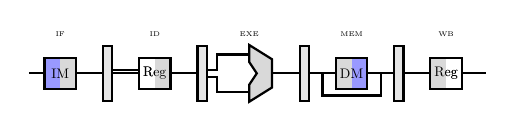
\begin{tikzpicture}[scale=0.5, transform shape]
            % Define styles
            \tikzstyle{block} = [rectangle, draw, thick, minimum width=0.8cm, minimum height=0.8cm, inner sep=2pt]
            \tikzstyle{latch} = [rectangle, draw, thick, minimum width=0.12cm, minimum height=1.4cm, fill=gray!20]
            \tikzstyle{line} = [draw, thick]
            
            % Stage labels
            \node[above] at (0,0.8) {\tiny IF};
            \node[above] at (2.4,0.8) {\tiny ID};
            \node[above] at (4.8,0.8) {\tiny EXE};
            \node[above] at (7.4,0.8) {\tiny MEM};
            \node[above] at (9.8,0.8) {\tiny WB};
            
            % Single pipeline row components
            % Highlight IM for instruction fetch (READ - left side)
            \node[block, fill=white] (IM) at (0,0) {IM};
            \fill[blue!40] (IM.north west) -- (IM.north) -- (IM.south) -- (IM.south west) -- cycle;
            \fill[gray!30] (IM.north) -- (IM.north east) -- (IM.south east) -- (IM.south) -- cycle;
            \node[block, fill=none] at (0,0) {IM};
            
            \node[latch] (L1) at (1.2,0) {};
            
            \node[block, fill=white] (Reg1) at (2.4,0) {Reg};
            \fill[gray!30] (Reg1.north) -- (Reg1.north east) -- (Reg1.south east) -- (Reg1.south) -- cycle;
            \node[block, fill=none] at (2.4,0) {Reg};
            
            \node[latch] (L2) at (3.6,0) {};
            
            % ALU
            \begin{scope}[shift={(4.8,0)}, scale=1.2]
                \coordinate (toptopleft) at (0, 0.6);
                \coordinate (topbottomleft) at (0, 0.24);
                \coordinate (left) at (0.16, 0);
                \coordinate (bottomtopleft) at (0, -0.24);
                \coordinate (bottombottomleft) at (0, -0.6);
                \coordinate (topright) at (0.48, 0.3);
                \coordinate (bottomright) at (0.48, -0.3);
                \fill[gray!30] (toptopleft) -- (topbottomleft) -- (left) -- (bottomtopleft) -- (bottombottomleft) -- (bottomright) -- (topright) -- cycle;
                \draw[thick] (toptopleft) -- (topbottomleft) -- (left) -- (bottomtopleft) -- (bottombottomleft) -- (bottomright) -- (topright) -- cycle;
                \coordinate (alu_input1) at (0, 0.4);
                \coordinate (alu_input2) at (0, -0.4);
                \coordinate (alu_output) at (0.48, 0);
            \end{scope}
            
            \node[latch] (L3) at (6.2,0) {};
            
            % Highlight DM for data access (READ/WRITE - right side)
            \node[block, fill=white] (DM) at (7.4,0) {DM};
            \fill[gray!30] (DM.north west) -- (DM.north) -- (DM.south) -- (DM.south west) -- cycle;
            \fill[blue!40] (DM.north) -- (DM.north east) -- (DM.south east) -- (DM.south) -- cycle;
            \node[block, fill=none] at (7.4,0) {DM};
            
            \node[latch] (L4) at (8.6,0) {};
            
            \node[block, fill=white] (Reg2) at (9.8,0) {Reg};
            \fill[gray!30] (Reg2.north west) -- (Reg2.north) -- (Reg2.south) -- (Reg2.south west) -- cycle;
            \node[block, fill=none] at (9.8,0) {Reg};
            
            % Connections
            \draw[line] (-0.8,0) -- (IM.west);
            \draw[line] (IM.east) -- (L1.west);
            
            % Two inputs to first Reg (from different sources)
            \draw[line] ([yshift=2.4pt]L1.east) -- ([yshift=2.4pt]Reg1.west);
            \draw[line] (L1.east) -- (Reg1.west);
            
            \draw[line] (Reg1.east) -- (L2.west);
            
            % Two inputs to ALU
            \draw[line] ([yshift=2.4pt]L2.east) -- ++(0.24,0) |- (alu_input1);
            \draw[line] ([yshift=-2.4pt]L2.east) -- ++(0.24,0) |- (alu_input2);
            
            % ALU output to next latch
            \draw[line] (alu_output) -- (L3.west);
            
            % DM connections
            \draw[line] (L3.east) -- (DM.west);
            \draw[line] (DM.east) -- (L4.west);
            
            % Bypass around DM
            \draw[line] (L3.east) -- ($(L3.east)!0.5!(DM.west)$) -- ++(0, -0.56) -|
                        ($(L4.west)!0.5!(DM.east)$) -- (L4.west);
            
            \draw[line] (L4.east) -- (Reg2.west);
            \draw[line] (Reg2.east) -- ++(0.6,0);
        \end{tikzpicture}
    \end{columns}
\end{frame}

\begin{frame}{Pipeline Architecture}
\begin{center}
\begin{circuitikz}[scale=0.9, transform shape]
    % Define circuitikz component styles
    \tikzstyle{imem_block} = [muxdemux, muxdemux def={Lh=2, Rh=2, w=1.5, NL=1, NR=1, square pins=1},
                              external pins width=0, fill=white, align=center]
    \tikzstyle{regfile_block} = [muxdemux, muxdemux def={Lh=2, Rh=2, w=1.5, NL=3, NR=4, square pins=1},
                                 external pins width=0, fill=white, align=center]
    \tikzstyle{regfile_wb} = [muxdemux, muxdemux def={Lh=2, Rh=2, w=1.5, NL=1, NR=0, square pins=1},
                              external pins width=0, fill=white, align=center]
    \tikzstyle{alu_block} = [muxdemux, muxdemux def={Lh=2, Rh=1.5, NL=2, NR=1, w=1.2, inset w=0.5, inset Lh=1, inset Rh=0},
                            external pins width=0, fill=white]
    \tikzstyle{dmem_block} = [muxdemux, muxdemux def={Lh=2, Rh=2, w=1.5, NL=1, NR=1, square pins=1},
                              external pins width=0, fill=white, align=center]
    \tikzstyle{latch} = [draw, thick, fill=gray!20, minimum width=0.15cm, minimum height=1.8cm]
    \tikzstyle{line} = [draw, thick]

    % Stage labels at top
    \node[font=\footnotesize] at (0, 2) {IF};
    \node[font=\footnotesize] at (2.5, 2) {ID};
    \node[font=\footnotesize] at (5, 2) {EXE};
    \node[font=\footnotesize] at (7.5, 2) {MEM};
    \node[font=\footnotesize] at (10, 2) {WB};

    % Instruction Memory
    \node[imem_block] (IM) at (0,0) {IM};

    % Latch L1
    \node[latch, anchor=west] (L1) at ([xshift=3mm]IM.east) {};

    % Register File (first) - anchor at lpin 2
    \node[regfile_block, anchor=lpin 2] (Reg1) at ([xshift=3mm]L1.east) {Reg};

    % Latch L2
    \node[latch, anchor=west] (L2) at ([xshift=3mm]Reg1.east |- L1) {};

    % ALU
    \node[alu_block, anchor=west] (ALU) at ([xshift=3mm]L2.east) {};

    % Latch L3
    \node[latch, anchor=west] (L3) at ([xshift=3mm]ALU.east |- L1) {};

    % Data Memory
    \node[dmem_block, anchor=lpin 1] (DM) at ([xshift=3mm]L3.east) {DM};

    % Latch L4
    \node[latch, anchor=west] (L4) at ([xshift=3mm]DM.east |- L1) {};

    % Register File (second) - only 1 lpin, no rpin
    \node[regfile_wb, anchor=lpin 1] (Reg2) at ([xshift=3mm]L4.east) {Reg};

    % Connections - using pins for clean horizontal lines
    \draw[line] (IM.rpin 1) -- (L1.west);
    \draw[line] (L1.east) -- (Reg1.lpin 2);
    \draw[line] ([xshift=2mm]L1.east) |- (Reg1.lpin 1);

    \draw[line] (Reg1.rpin 1) -- (L2.west |- Reg1.rpin 1);
    \draw[line] (Reg1.rpin 4) -- (L2.west |- Reg1.rpin 4);

    \draw[line] (L2.east |- ALU.lpin 1) -- (ALU.lpin 1);
    \draw[line] (L2.east |- ALU.lpin 2) -- (ALU.lpin 2);

    \draw[line] (ALU.rpin 1) -- (L3.west);

    \draw[line] (L3.east) -- (DM.lpin 1);
    \draw[line] (DM.rpin 1) -- (L4.west);

    % Bypass around DM
    \draw[line] (L3.east) -- ++(2mm, 0) coordinate (bypass_start) -| ([xshift=-1mm, yshift=-1mm]DM.south west) -| ([xshift=1mm,yshift=-3mm]DM.east) -- ([yshift=-3mm]L4.west);

    \draw[line] (L4.east) -- (Reg2.lpin 1);

\end{circuitikz}
\end{center}
\end{frame}

%% Slide: Pipeline Example
\begin{frame}{Pipeline Example: cycle 1}
    \begin{columns}
        \column{0.4\textwidth}
        \begin{tabular}{ll}
            0 & \texttt{lw R10,9(R1)}\\
            4 & \texttt{sub R11,R2,R3}\\
            8 & \texttt{and R12,R4,R5}\\
            12 & \texttt{or R13,R6,R7}
        \end{tabular}
        
        \column{0.6\textwidth}
        \centering
        PC = 0
        \vspace{0.5cm}
        
        \begin{tikzpicture}[scale=0.6]
            \node[draw, dashed, minimum width=8cm, minimum height=3cm, align=center] {
                Pipeline State Diagram\\
                (Cycle 1)
            };
        \end{tikzpicture}
    \end{columns}
\end{frame}

%% Slide: RAW Dependency
\begin{frame}{RAW Dependency}
    \begin{columns}
        \column{0.5\textwidth}
        Program execution order:
        \begin{enumerate}
            \item \texttt{sub R2, R1, R3}
            \item \texttt{and R12, \textcolor{red}{R2}, R5}
            \item \texttt{or R13, R6, \textcolor{red}{R2}}
            \item \texttt{add R14, \textcolor{red}{R2}, \textcolor{red}{R2}}
            \item \texttt{sw R15, 100(\textcolor{red}{R2})}
        \end{enumerate}
        
        \column{0.5\textwidth}
        \centering
        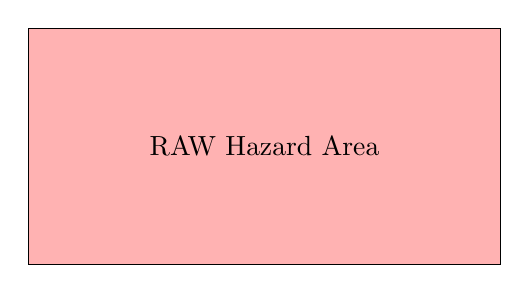
\begin{tikzpicture}[scale=0.5]
            % Pipeline stages showing dependency
            \node[draw, fill=red!30, minimum width=6cm, minimum height=3cm] {
                RAW Hazard Area
            };
        \end{tikzpicture}
    \end{columns}
\end{frame}

%% Slide: Using Bypass to Solve RAW Dependency
\begin{frame}{Using Bypass to Solve RAW Dependency}
    \begin{itemize}
        \item Bypass result directly from EXE output to EXE input
        \item No stall needed when bypass is possible
        \item Hardware forwards data from:
        \begin{itemize}
            \item EXE/MEM pipeline register
            \item MEM/WB pipeline register
        \end{itemize}
    \end{itemize}
    
    \centering
    \begin{tikzpicture}[scale=0.7]
        \node[draw, dashed, minimum width=10cm, minimum height=4cm] {
            Bypass/Forwarding Hardware Diagram
        };
    \end{tikzpicture}
\end{frame}

%% Slide: Bypass Control
\begin{frame}[fragile]{Bypass Control}
    \textbf{L3\_reg\_wr = L3.RegWrite and (L3.opcode != lw)}
    
    \vspace{0.3cm}
    \textbf{Forwarding from EXE (L3):}
    \begin{itemize}
        \item \small if (L3\_reg\_wr and (L3.dst == L2.src1)) ALUSelA = 1
        \item \small if (L3\_reg\_wr and (L3.dst == L2.src2)) ALUSelB = 1
    \end{itemize}
    
    \vspace{0.3cm}
    \textbf{Forwarding from MEM (L4):}
    \begin{itemize}
        \item \small if (L4.RegWrite and ((not L3\_reg\_wr) or (L3.dst $\neq$ L2.src1))\\
              and (L4.dst = L2.src1)) ALUSelA = 2
        \item \small if (L4.RegWrite and ((not L3\_reg\_wr) or (L3.dst $\neq$ L2.src2))\\
              and (L4.dst = L2.src2)) ALUSelB = 2
    \end{itemize}
\end{frame}

% Macro for drawing full pipeline architecture based on Pipeline Architecture slide
\pgfkeys{
    /pipelinearch/.is family, /pipelinearch,
    default/.style = {
        prefix = pipe,
        at = {(0,0)},
        scale = 0.5
    },
    prefix/.estore in = \pipeprefix,
    at/.store in = \pipeat,
    scale/.estore in = \pipescale
}

\newcommand{\drawpipelinearch}[1][]{%
    \pgfkeys{/pipelinearch, default, #1}%
    \begin{scope}[scale=\pipescale, transform shape]
        % Define circuitikz component styles (EXACTLY as Pipeline Architecture)
        \tikzstyle{imem_block} = [muxdemux, muxdemux def={Lh=2, Rh=2, w=1.5, NL=1, NR=1, square pins=1},
                                  external pins width=0, fill=white, align=center]
        \tikzstyle{regfile_block} = [muxdemux, muxdemux def={Lh=2, Rh=2, w=1.5, NL=3, NR=4, square pins=1},
                                     external pins width=0, fill=white, align=center]
        \tikzstyle{regfile_wb} = [muxdemux, muxdemux def={Lh=2, Rh=2, w=1.5, NL=1, NR=0, square pins=1},
                                  external pins width=0, fill=white, align=center]
        \tikzstyle{alu_block} = [muxdemux, muxdemux def={Lh=2, Rh=1.5, NL=2, NR=1, w=1.2, inset w=0.5, inset Lh=1, inset Rh=0},
                                external pins width=0, fill=white]
        \tikzstyle{dmem_block} = [muxdemux, muxdemux def={Lh=2, Rh=2, w=1.5, NL=1, NR=1, square pins=1},
                                  external pins width=0, fill=white, align=center]
        \tikzstyle{latch} = [draw, thick, fill=gray!20, minimum width=0.15cm, minimum height=1.4cm]
        \tikzstyle{line} = [draw, thick]

        % Instruction Memory - positioned at the 'at' coordinate
        \node[imem_block] (\pipeprefix-IM) at \pipeat {IM};

        % Latch L1
        \node[latch, anchor=west] (\pipeprefix-L1) at ([xshift=3mm]\pipeprefix-IM.east) {};

        % Register File (first) - anchor at lpin 2
        \node[regfile_block, anchor=lpin 2] (\pipeprefix-Reg1) at ([xshift=3mm]\pipeprefix-L1.east) {Reg};

        % Latch L2 - aligned with L1 vertically
        \node[latch, anchor=west] (\pipeprefix-L2) at ([xshift=3mm]\pipeprefix-Reg1.east |- \pipeprefix-L1) {};

        % ALU - using anchor=west like the original
        \node[alu_block, anchor=west] (\pipeprefix-ALU) at ([xshift=3mm]\pipeprefix-L2.east) {};

        % Latch L3 - aligned with L1 vertically
        \node[latch, anchor=west] (\pipeprefix-L3) at ([xshift=3mm]\pipeprefix-ALU.east |- \pipeprefix-L1) {};

        % Data Memory
        \node[dmem_block, anchor=lpin 1] (\pipeprefix-DM) at ([xshift=3mm]\pipeprefix-L3.east) {DM};

        % Latch L4 - aligned with L1 vertically
        \node[latch, anchor=west] (\pipeprefix-L4) at ([xshift=3mm]\pipeprefix-DM.east |- \pipeprefix-L1) {};

        % Register File (second) - only 1 lpin, no rpin
        \node[regfile_wb, anchor=lpin 1] (\pipeprefix-Reg2) at ([xshift=3mm]\pipeprefix-L4.east) {Reg};

        % Connections - EXACTLY as Pipeline Architecture
        \draw[line] (\pipeprefix-IM.rpin 1) -- (\pipeprefix-L1.west);
        \draw[line] (\pipeprefix-L1.east) -- (\pipeprefix-Reg1.lpin 2);
        \draw[line] ([xshift=2mm]\pipeprefix-L1.east) |- (\pipeprefix-Reg1.lpin 1);

        \draw[line] (\pipeprefix-Reg1.rpin 1) -- (\pipeprefix-L2.west |- \pipeprefix-Reg1.rpin 1);
        \draw[line] (\pipeprefix-Reg1.rpin 4) -- (\pipeprefix-L2.west |- \pipeprefix-Reg1.rpin 4);

        \draw[line] (\pipeprefix-L2.east |- \pipeprefix-ALU.lpin 1) -- (\pipeprefix-ALU.lpin 1);
        \draw[line] (\pipeprefix-L2.east |- \pipeprefix-ALU.lpin 2) -- (\pipeprefix-ALU.lpin 2);

        \draw[line] (\pipeprefix-ALU.rpin 1) -- (\pipeprefix-L3.west);

        \draw[line] (\pipeprefix-L3.east) -- (\pipeprefix-DM.lpin 1);
        \draw[line] (\pipeprefix-DM.rpin 1) -- (\pipeprefix-L4.west);

        % Bypass around DM - EXACTLY as Pipeline Architecture
        \draw[line] (\pipeprefix-L3.east) -- ++(2mm, 0) coordinate (\pipeprefix-bypass_start) -| ([xshift=-1mm, yshift=-1mm]\pipeprefix-DM.south west) -| ([xshift=1mm,yshift=-3mm]\pipeprefix-DM.east) -- ([yshift=-3mm]\pipeprefix-L4.west);

        \draw[line] (\pipeprefix-L4.east) -- (\pipeprefix-Reg2.lpin 1);
    \end{scope}
}

%% Slide: Register File Split
\begin{frame}{Register File Split}
    \begin{itemize}
        \item Register file is written during first half of the cycle
        \item Register file is read during second half of the cycle
        \item[$\Rightarrow$] Register file is written before it is read $\Rightarrow$ returns the correct data
    \end{itemize}

    \vspace{0.3cm}
    \centering
    \begin{circuitikz}[scale=0.9, transform shape]
        % Timeline at top
        \node[anchor=south west, font=\small] at (-1.5, 3.2) {Time (clock cycles)};
        \draw[->, thick] (0, 3) -- (10, 3);
        \foreach \i in {1,...,9} {
            \node[above, font=\scriptsize] at (\i, 3) (i\i) {\i};
        }

        % Instructions with named nodes
        \node[anchor=east, font=\small\ttfamily] (lw_inst) at (-0.3, 2) {lw R2, 30(R1)};
        \node[anchor=east, font=\small\ttfamily, anchor=north east] (and_inst) at ([yshift=-3mm]lw_inst.south east) {and R12, R2, R5};
        \node[anchor=east, font=\small\ttfamily, anchor=north east] (or_inst) at ([yshift=-3mm]and_inst.south east) {or R13, R6, R2};
        \node[anchor=east, font=\small\ttfamily, anchor=north east] (add_inst) at ([yshift=-3mm]or_inst.south east) {add R14, R2, R2};
        \node[anchor=east, font=\small\ttfamily, anchor=north east] (sw_inst) at ([yshift=-3mm]add_inst.south east) {sw R15, 100(R2)};

        \drawpipelinearch[prefix=i1, at={(lw_inst -| i1)}, scale=0.58]
        \drawpipelinearch[prefix=i1, at={(and_inst -| i2)}, scale=0.58]
        \drawpipelinearch[prefix=i1, at={(or_inst -| i3)}, scale=0.58]
        \drawpipelinearch[prefix=i1, at={(add_inst -| i4)}, scale=0.58]
        \drawpipelinearch[prefix=i1, at={(sw_inst -| i5)}, scale=0.58]

        % Program execution order label with arrow
        \node[anchor=south east, align=center, font=\small] at (lw_inst.north west) (ordertext) {Program\\execution\\order};
        \draw[->, thick] (ordertext.south) -- (ordertext |- sw_inst);
    \end{circuitikz}
\end{frame}

%% Slide: Can't Always Bypass
\begin{frame}{Can't Always Bypass}
    \begin{itemize}
        \item Load word can still cause a hazard
        \begin{itemize}
            \item An instruction tries to read a register following a load instruction that writes to the same register
        \end{itemize}
        \item A hazard detection unit is needed to "stall" the load instruction
    \end{itemize}
    
    Program execution order:
    \begin{enumerate}
        \item \texttt{lw \textcolor{red}{R2}, 30(R1)}
        \item \texttt{and R12, \textcolor{red}{R2}, R5}
        \item \texttt{or R13, R6, \textcolor{red}{R2}}
        \item \texttt{add R14, \textcolor{red}{R2}, \textcolor{red}{R2}}
        \item \texttt{sw R15, 100(\textcolor{red}{R2})}
    \end{enumerate}
\end{frame}

%% Slide: Stall If Cannot Bypass
\begin{frame}[fragile]{Stall If Cannot Bypass}
\begin{minted}{text}
if (L2.RegWrite and (L2.opcode == lw) and
    ((L2.dst == L1.src1) or (L2.dst == L1.src2)))
then stall
\end{minted}
    
    \vspace{0.3cm}
    \begin{itemize}
        \item De-assert the enable to the L1 latch, and to the IP
        \begin{itemize}
            \item The dependent instruction (and) stays another cycle in L1
        \end{itemize}
        \item Issue a NOP into the L2 latch (instead of the stalled inst.)
        \item Allow the stalling instruction (lw) to move on
    \end{itemize}

    \vspace{0.3cm}
    \centering
    \begin{circuitikz}[scale=1, transform shape]
        % Timeline at top
        \node[anchor=south, font=\small] at (4.5, 2.8) {Time (clock cycles)};
        \draw[->, thick] (0, 2.5) -- (9.5, 2.5);
        \foreach \i in {1,...,9} {
            \node[above, font=\scriptsize] at (\i*1, 2.5) {\i};
        }

        % Program execution order label
        \node[anchor=north, align=center, font=\small] at (-0.8, 2.3) {Program\\execution\\order};

        % Instructions
        \node[anchor=east, font=\small\ttfamily] at (0, 2) {lw \textcolor{blue}{R2}, 30(R1)};
        \node[anchor=east, font=\small\ttfamily] at (0, 1) {and R12,\textcolor{blue}{R2}, R5};
        \node[anchor=east, font=\small\ttfamily] at (0, 0) {or R13,R6, \textcolor{blue}{R2}};
        \node[anchor=east, font=\small\ttfamily] at (0, -1) {add R14,\textcolor{blue}{R2}, \textcolor{blue}{R2}};
        \node[anchor=east, font=\small\ttfamily] at (0, -2) {sw R15,100(\textcolor{blue}{R2})};

        % Draw pipeline stages using the macro
        % lw instruction - cycle 1
        \drawpipelinearch[prefix=lw, at={(1,2)}, scale=0.5]

        % and instruction - cycle 2
        \drawpipelinearch[prefix=and1, at={(2,1)}, scale=0.5]

        % bubble - cycle 3 at row 2 (and's position)
        \node[draw, fill=gray!30, minimum width=0.5cm, minimum height=0.3cm, font=\tiny, anchor=west] at (3, 1) {bubble};

        % and instruction continues - cycle 4
        \drawpipelinearch[prefix=and2, at={(4,1)}, scale=0.5]

        % or instruction - cycle 3
        \drawpipelinearch[prefix=or, at={(3,0)}, scale=0.5]

        % add instruction - cycle 4
        \drawpipelinearch[prefix=add, at={(4,-1)}, scale=0.5]

        % sw instruction - cycle 5
        \drawpipelinearch[prefix=sw, at={(5,-2)}, scale=0.5]
    \end{circuitikz}
\end{frame}

%% Slide: Software Scheduling to Avoid Load Hazards
\begin{frame}[fragile]{Software Scheduling to Avoid Load Hazards}
    \begin{tikzpicture}[remember picture, overlay]
        % Calculate base position
        \coordinate (base) at ($(current page.north) + (0, -1.5)$);

        % Example C code (left column)
        \node[anchor=north west, align=left] (example) at ($(base) + (-7, 0)$) {
            Example: code for (assume all\\
            variables are in memory):
        };
        \node[anchor=north west, font=\ttfamily, align=left] (c_code) at ($(example.south west) + (-0, -0.1)$) {
            a = b + c;\\
            d = e - f;
        };

        % Slow code column
        \node[anchor=north west, align=left] (slow_title) at ($(base) + (-0.5, 0)$) {\textbf{Slow code}};
        \draw (slow_title.south west) -- (slow_title.south east);

        \node[anchor=north west, font=\small\ttfamily, align=left] (slow_code) at ($(slow_title.south west) + (0, -0.1)$) {
            LW~~~Rb,b\\
            LW~~~\textcolor{red}{Rc},c\\
            \textcolor{blue}{Stall}\\
            ADD~~Ra,Rb,\textcolor{red}{Rc}\\
            \tikzmark{slow_sw1}SW~~~a,Ra\\
            \tikzmark{slow_re}LW~~~Re,e\\
            LW~~~\textcolor{red}{Rf},f\\
            \textcolor{blue}{Stall}\\
            SUB~~Rd,Re,\textcolor{red}{Rf}\\
            SW~~~d,Rd
        };

        % Fast code column
        \node[anchor=north west, align=left] (fast_title) at ($(base) + (3.5, 0)$) {\textbf{Fast code}};
        \draw (fast_title.south west) -- (fast_title.south east);

        \node[anchor=north west, font=\small\ttfamily, align=left] (fast_code) at ($(fast_title.south west) + (0, -0.1)$) {
            LW~~~Rb,b\\
            LW~~~Rc,c\\
            \tikzmark{fast_re}LW~~~\textcolor{green!60!black}{Re,e}\\
            ADD~~Ra,Rb,Rc\\
            LW~~~Rf,f\\
            \tikzmark{fast_sw1}SW~~~\textcolor{green!60!black}{a,Ra}\\
            SUB~~Rd,Re,Rf\\
            SW~~~d,Rd
        };

        % Arrows using tikzmark
        \begin{scope}[overlay, remember picture]
            % Arrow from slow LW Re,e to fast LW Re,e
            \draw[->, thick] ($(pic cs:slow_re) + (2.2, 0.1)$) to[out=0, in=180] ($(pic cs:fast_re) + (-0.3, 0.1)$);

            % Arrow from slow SW a,Ra to fast SW a,Ra
            \draw[->, thick] ($(pic cs:slow_sw1) + (2.2, 0.1)$) to[out=0, in=180] ($(pic cs:fast_sw1) + (-0.3, 0.1)$);
        \end{scope}

        % Bottom text
        \node[anchor=north, align=center] at ($(current page.south) + (0, 1.2)$) {
            {\large Instruction order can be changed \underline{as long as} the correctness is kept}
        };
    \end{tikzpicture}
\end{frame}

%% Slide: Control Hazard on Branches (based on BTB slide structure but without BTB)
\begin{frame}<1-4>[label=control-hazard]{Control Hazard on Branches}
\begin{center}
\scalebox{0.58}{
\begin{circuitikz}[
    % Component styles matching BTB slide exactly
    component/.style={draw, thick, minimum height=0.8cm},
    pipeline_reg/.style={draw, thick, fill=gray!20, minimum width=6mm, minimum height=5.8cm},
    stage_label/.style={draw, thick, fill=blue!60, text=white, font=\bfseries, minimum width=1.2cm, minimum height=0.5cm, text depth=0.25ex},
    imem_block/.style={muxdemux, muxdemux def={Lh=3, NL=3, Rh=3, NR=3, w=3.6, square pins=1},
                        external pins width=0, align=center, text depth=3ex, fill=yellow!20},
    regfile/.style={muxdemux, muxdemux def={Lh=4, NL=4, Rh=4, NR=2, w=2.8, square pins=1},
                    external pins width=0, fill=cyan!20, align=center},
    alu_style/.style={muxdemux, muxdemux def={Lh=2.6, Rh=1.5, NL=2, NR=5, NB=1, w=1.3, inset w=0.5, inset Lh=2, inset Rh=0, square pins=1},
                     external pins width=0, fill=green!20, font=\scriptsize},
    adder/.style={muxdemux, muxdemux def={Lh=1.2, NL=2, Rh=0.6, NR=1, w=1, inset w=0.3, inset Lh=0.6, inset Rh=0, square pins=1},
                     external pins width=0, fill=cyan!20, font=\scriptsize},
    mux2/.style={muxdemux, muxdemux def={Lh=1.6, Rh=0.8, NL=2, NR=1, NB=1, w=0.8},
                 external pins width=0, fill=cyan!20},
    pcsrc_mux/.style={muxdemux, muxdemux def={Lh=0.8, Rh=1.6, NL=1, NR=2, NT=1, w=0.8},
                 external pins width=0, fill=cyan!20},
    arrow/.style={->, >=stealth, thick},
    data_path/.style={arrow, black},
    repair_path/.style={arrow, red!70!black},
    line_label/.style={above, inner sep=1pt, font=\footnotesize},
    next_seq_label/.style={line_label, midway},
    repair_label/.style={line_label, text=red!70!black},
    lpin_label/.style={align=left, anchor=west, font=\tiny},
    rpin_label/.style={align=right, anchor=east, font=\tiny},
    data_connector/.style={circle, fill, inner sep=1.2pt},
    data_latch/.style={draw, thick, fill=cyan!20, minimum width=6mm, minimum height=0.3cm, inner sep=1pt, font=\tiny},
    inst_label/.style={draw, fill=orange!40, rounded corners=2pt, font=\scriptsize\ttfamily, inner sep=2pt},
    node distance=5mm and 5mm,
]

% IF Stage Components (same positioning as BTB slide)
\node[component, fill=yellow!30, minimum width=0.8cm] (PC) {IP};
\node[imem_block, right=of PC, anchor=blpin 2] (IMem) {Inst.\\Cache};
\node[adder, above=2mm of IMem.north, anchor=south] (PCadder) {+};
\node[pcsrc_mux, anchor=south] (PCSrcMux) at ([yshift=17mm]IMem.north west) {};
\node[font=\scriptsize, left=5mm of PCadder.blpin 2] (four) {4};

% Pipeline register IF/ID
\node[pipeline_reg, right=8mm of IMem.brpin 2] (IFID) {};
\node[data_latch, minimum height=2cm] (Instruction) at (IMem.rpin 2 -| IFID) {\rotatebox{90}{Instruction}};

% ID Stage Components
\node[regfile, right=15mm of IFID] (RegFile) {\rotatebox{90}{Register File}};

% Sign Extend unit
\node[ellipse, draw, thick, fill=cyan!20, minimum width=0.3cm, minimum height=0.2cm, inner sep=0pt,
      font=\tiny, below=2mm of RegFile.south] (SignExt) {\rotatebox{90}{SignExt}};

% Pipeline register ID/EX
\node[pipeline_reg, right=8mm of RegFile.east |- IFID] (IDEX) {};

% EX Stage Components - ALU and MUX for immediate selection
\node[alu_style, anchor=blpin 1] (ALU) at ([xshift=2cm]RegFile.brpin 1 -| IDEX.east) {};
\node[mux2, anchor=rpin 1] (ALUMux) at ([xshift=-4mm]ALU.lpin 2) {};
\node[font=\scriptsize, below right=-2mm of ALU.blpin 1] {\rotatebox{-45}{ALU}};

% Target calculation adder
\node[adder, anchor=lpin 1] (TargetAdder) at ([xshift=-5mm]ALU.west |- PCadder.rpin 1) {+};

% Pipeline register EX/MEM
\node[pipeline_reg, right=12mm of ALU.east |- IDEX] (EXMEM) {};

% MEM Stage Components
\node[muxdemux, muxdemux def={Lh=4.1, NL=10, Rh=4.1, NR=10, w=2.8, square pins=1},
      external pins width=0, align=center, text depth=6.5ex, fill=yellow!20, anchor=lpin 5] (DMem) at ([xshift=1cm]ALU.brpin 4 -| EXMEM.east) {Data\\Cache};

% Pipeline register MEM/WB
\node[pipeline_reg, right=8mm of DMem.east |- EXMEM] (MEMWB) {};

% WB Stage
\node[mux2, anchor=lpin 1] at ([xshift=8mm]MEMWB.east |- DMem.rpin 5) (WBMux) {};

% Stage labels (same positioning as BTB slide - relative to IMem.north)
\node[stage_label] (IF_label) at ([yshift=37mm]IMem.north) {Fetch};
\node[stage_label] (ID_label) at (IF_label -| RegFile) {Decode};
\node[stage_label] (EX_label) at (IF_label -| ALU) {Execute};
\node[stage_label] (MEM_label) at (IF_label -| DMem) {Memory};
\node[stage_label] (WB_label) at (IF_label -| WBMux) {WB};

% === Routing coordinates for pipeline signal propagation ===
% Next sequential address coordinates
\coordinate (fetch_out_next_seq) at (PCadder.brpin 1 -| IFID.west);
\coordinate (decode_in_next_seq) at (IFID.east |- fetch_out_next_seq);
\coordinate (decode_out_next_seq) at (IDEX.west |- fetch_out_next_seq);
\coordinate (execute_in_next_seq) at (IDEX.east |- fetch_out_next_seq);

% Target register coordinates
\coordinate (decode_out_target_reg) at ([yshift=-2mm]IDEX.west |- SignExt.south);
\coordinate (execute_in_target_reg) at (decode_out_target_reg -| IDEX.east);
\coordinate (execute_out_target_reg) at (decode_out_target_reg -| EXMEM.west);
\coordinate (mem_in_target_reg) at (decode_out_target_reg -| EXMEM.east);
\coordinate (mem_out_target_reg) at (decode_out_target_reg -| MEMWB.west);
\coordinate (wb_in_target_reg) at (decode_out_target_reg -| MEMWB.east);

% === Data paths (same as BTB slide) ===
% MUX output to PC
\coordinate (IP_west_conn) at ([xshift=-5mm]PC.west);
\draw[data_path] (PCSrcMux.lpin 1) -| (IP_west_conn) -- (PC.west);
\draw[data_path] (PC.east) -- (IMem.blpin 2);

% PC to adder
\node[data_connector] (PC_conn) at ([xshift=3mm]PC.east) {};
\draw[data_path] (PC_conn) |- (PCadder.blpin 1);
\draw[data_path] (four.east) -- (PCadder.blpin 2);

% === Next sequential address ===
\draw[data_path] (PCadder.brpin 1) -- ++(4mm,0) node[data_connector] (NextSeqConn) {} -- ++(0.1,0) |- (fetch_out_next_seq);
\draw[data_path] (NextSeqConn) |- (PCSrcMux.rpin 2);
\draw[data_path] (decode_in_next_seq) -- node[next_seq_label] {next sequential address} (decode_out_next_seq);
\draw[data_path] (execute_in_next_seq) |- (TargetAdder.lpin 1);

% IMem to IF/ID
\draw[data_path] (IMem.brpin 2) -- (IFID.west |- IMem.brpin 2);

% IF/ID to RegFile
\draw[data_path] (IFID.east |- RegFile.lpin 1) -- (RegFile.blpin 1);
\draw[data_path] (IFID.east |- RegFile.lpin 2) -- (RegFile.blpin 2);

% RegFile to ID/EX
\draw[data_path] (RegFile.brpin 1) -- (IDEX.west |- RegFile.brpin 1);
\draw[data_path] (RegFile.brpin 2) -- (IDEX.west |- RegFile.brpin 2);

% IF/ID to Sign Extend
\draw[data_path] (IFID.east |- SignExt) -- (SignExt.west);
% Sign Extend to ID/EX
\draw[data_path] (SignExt.east) -- (IDEX.west |- SignExt);

% ID/EX to ALU (top input direct, bottom through MUX)
\draw[data_path] (IDEX.east |- ALU.blpin 1) -- (ALU.blpin 1);
\coordinate (WriteDataJunction) at ([xshift=-3mm]ALUMux.lpin 1);
\draw[data_path] (IDEX.east |- ALUMux.lpin 1) -- (WriteDataJunction) node[data_connector] {} -- (ALUMux.blpin 1);
\draw[data_path] (WriteDataJunction) |- (EXMEM.west |- DMem.lpin 10);
\draw[data_path] (EXMEM.east |- DMem.lpin 10) -- (DMem.lpin 10);
\draw[data_path] (ALUMux.rpin 1) -- (ALU.blpin 2);

% SignExt through ID/EX to ALUMux and Target Adder
\coordinate (ImmJunction) at ([xshift=-7mm]ALUMux.lpin 2);
\draw[data_path] (SignExt -| IDEX.east) -| (ImmJunction) -- (ALUMux.lpin 2);
\node[data_connector] at (ImmJunction) {};
\draw[data_path] (ImmJunction) |- (TargetAdder.blpin 2);

% Target Adder to EX/MEM buffer
\coordinate (calc_target_exmem) at (TargetAdder.brpin 1 -| EXMEM);
\draw[arrow, green!60!black] (TargetAdder.brpin 1) -- node[midway, line_label, text=green!60!black] {calc.\ target} (calc_target_exmem);

% ALU outputs to EX/MEM buffer
\coordinate (exmem_alu_zero) at (ALU.brpin 2 -| EXMEM.west);
\coordinate (exmem_alu_result) at (ALU.brpin 4 -| EXMEM.west);
\draw[arrow, orange!70!black] (ALU.brpin 2) -- node[midway, line_label, text=orange!70!black] {zero} (exmem_alu_zero);
\draw[data_path] (ALU.brpin 4) -- node[midway, line_label] {result} (exmem_alu_result);

% EX/MEM to DMem (addr)
\draw[data_path] (EXMEM.east |- DMem.lpin 5) -- (DMem.lpin 5);

% DMem to MEM/WB (read data)
\draw[data_path] (DMem.rpin 5) -- (MEMWB.west |- DMem.rpin 5);

% Instruction propagation through pipeline
\draw[data_path] ([yshift=8mm]Instruction.south east) -- ++(0.5,0) |- (decode_out_target_reg);
\draw[data_path] (execute_in_target_reg) -- (execute_out_target_reg);
\draw[data_path] (mem_in_target_reg) -- (mem_out_target_reg);
\draw[data_path] (wb_in_target_reg) -- ++(0.5,0) |- ([yshift=-5mm,xshift=-6mm]RegFile.west |- IDEX.south) |- (RegFile.blpin 3);

% MEM/WB to WB Mux
\draw[data_path] (MEMWB.east |- WBMux.lpin 1) -- (WBMux.blpin 1);

% Address path from DMem to WB Mux
\coordinate (AddrWB) at ([yshift=-3mm]DMem.south -| MEMWB.west);
\node[data_connector] (AddrConn) at ([xshift=-5mm]DMem.lpin 5) {};
\draw[data_path] (AddrConn) |- (AddrWB);
\draw[data_path] (AddrWB -| MEMWB.east) -- ++(0.5,0) |- (WBMux.lpin 2);

% WB Mux output to Register File write data
\draw[data_path] (WBMux.rpin 1) -- ++(0.5,0) |- ([xshift=-4mm,yshift=-8mm]IDEX.south -| RegFile.lpin 4) |- (RegFile.blpin 4);

% === Branch target path (from calc target back to PC mux) - highlighted ===
\coordinate (calc_target_mem_out) at (calc_target_exmem -| EXMEM.east);
\draw[arrow, blue!70!black, line width=1.5pt] (calc_target_mem_out) -- ++(0.5,0) |- (PCSrcMux.rpin 1);

% === Zero (branch taken) signal to mux select ===
\coordinate (zero_mem_out) at (exmem_alu_zero -| EXMEM.east);
\draw[arrow, orange!70!black, line width=1.5pt] (zero_mem_out) -- ++(7mm,0) |- ([yshift=3mm]PCSrcMux.north) -- (PCSrcMux.tpin 1);

% Register File labels
\node[align=left, xshift=3mm, font=\tiny] at (RegFile.blpin 1) {read\\reg 1};
\node[align=left, xshift=3mm, font=\tiny] at (RegFile.blpin 2) {read\\reg 2};
\node[align=left, xshift=3mm, font=\tiny] at (RegFile.blpin 3) {write\\reg};
\node[align=left, xshift=3mm, font=\tiny] at (RegFile.blpin 4) {write\\data};
\node[align=right, xshift=-3mm, font=\tiny] at (RegFile.brpin 1) {read\\data 1};
\node[align=right, xshift=-3mm, font=\tiny] at (RegFile.brpin 2) {read\\data 2};

% Data Cache labels
\node[align=left, font=\tiny] at ([xshift=3mm,yshift=-1mm]DMem.lpin 5) {addr};
\node[align=left, font=\tiny] at ([xshift=3mm, yshift=2mm]DMem.lpin 10) {write\\data};
\node[align=right, font=\tiny] at ([xshift=-3mm,yshift=-2mm]DMem.rpin 5) {read\\data};

% === Styles for instructions and values ===
\tikzset{
    latch_inst/.style={draw=blue!70!black, line width=1.5pt, fill=blue!15,
                       rounded corners=3pt, font=\small\bfseries\ttfamily, inner sep=4pt,
                       minimum height=5mm, text depth=0.5ex},
    latch_inst_flush/.style={draw=red!70!black, line width=2pt, fill=red!30,
                       rounded corners=3pt, font=\small\bfseries\ttfamily, inner sep=4pt,
                       minimum height=5mm, text depth=0.5ex},
    latch_nextseq/.style={draw=gray!60!black, line width=1pt, fill=gray!20,
                          rounded corners=3pt, font=\small\bfseries, inner sep=3pt},
    latch_offset/.style={draw=cyan!60!black, line width=1pt, fill=cyan!15,
                          rounded corners=2pt, font=\scriptsize\bfseries, inner sep=2pt},
    latch_target/.style={draw=green!60!black, line width=1pt, fill=green!25,
                          rounded corners=3pt, font=\small\bfseries, inner sep=3pt},
    ip_value/.style={font=\small\bfseries, text=blue!70!black},
    stage_box/.style={draw=blue!50!black, line width=1.5pt, fill=blue!8,
                      rounded corners=6pt, font=\small, inner sep=8pt},
}

% Program listing with border (right side, same as BTB slide)
\node[draw, thick, fill=white, rounded corners=3pt, inner sep=4pt,
      anchor=north west, font=\small\ttfamily, align=left]
      (ProgramListing) at ([xshift=5mm]WBMux.east |- IF_label.south) {
    \begin{tabular}{rl}
    0: & or \\
    4: & jcc 50 \\
    8: & and \\
    12: & sw \\
    16: & sub \\
    \end{tabular}
};

% Coordinate for explanation box at bottom of page
\coordinate (StageExplainPos) at ([yshift=-38mm]IMem.south -| RegFile);

% Style for consistent explanation box
\tikzset{
    explain_box/.style={draw=green!50!black, line width=1.5pt, fill=green!10, rounded corners=6pt,
                        font=\small, inner sep=8pt, anchor=west, align=left},
}

% === Slide 1: Empty pipeline, explain jcc (PPT slide 30) ===
\only<1>{
    \node[explain_box] at (StageExplainPos) {
        \textbf{jcc target; if cond then PC $\leftarrow$ target}\\[2mm]
        $\diamond$ The target is saved in the instruction relative to the address of the fall-through instruction\\
        $\diamond$ Most conditional jumps are short (if and loop) $\Rightarrow$ save bits in the instruction encoding
    };
}

% === Slide 2: PC=8, jcc at IF/ID, or at ID/EX (PPT slide 31) ===
\only<2>{
    \node[ip_value] at ([yshift=-3mm]PC.south) {8};
    % Instructions
    \node[latch_inst] (jcc2) at (Instruction.south) {jcc};
    \node[latch_offset, anchor=north] at ([yshift=-1mm]jcc2.south) {42};
    \node[latch_inst] at (IDEX.center |- Instruction.south) {or};
    % Values
    \node[latch_nextseq] at (IFID.center |- fetch_out_next_seq) {8};
    \node[latch_nextseq] at (IDEX.center |- decode_out_next_seq) {4};
    % Explanation
    \node[explain_box] at (StageExplainPos) {
        \textbf{jcc target; if cond then PC $\leftarrow$ target}\\[2mm]
        $\diamond$ The target is saved in the instruction relative to the address of the fall-through instruction\\
        $\diamond$ Most conditional jumps are short (if and loop) $\Rightarrow$ save bits in the instruction encoding
    };
}

% === Slide 3: IP=12, jcc at ID/EX, and at IF/ID, or at EX/MEM (PPT slide 32) ===
\only<3>{
    \node[ip_value] at ([yshift=-3mm]PC.south) {12};
    % Instructions
    \node[latch_inst] at (Instruction.south) {and};
    \node[latch_inst] (jcc3) at (IDEX.center |- Instruction.south) {jcc};
    \node[latch_offset, anchor=north] at ([yshift=-1mm]jcc3.south) {42};
    \node[latch_inst] at (EXMEM.center |- Instruction.south) {or};
    % Values
    \node[latch_nextseq] at (IFID.center |- fetch_out_next_seq) {12};
    \node[latch_nextseq] at (IDEX.center |- decode_out_next_seq) {8};
    \node[latch_target] at (calc_target_exmem) {50};
    % Explanation
    \node[explain_box] at (StageExplainPos) {
        Instructions following the branch get into the pipe
    };
}

% === Slide 4: PC=16, jcc at EX/MEM (PPT slide 33) ===
\only<4>{
    \node[ip_value] at ([yshift=-3mm]PC.south) {16};
    % Instructions
    \node[latch_inst] at (Instruction.south) {sw};
    \node[latch_inst] at (IDEX.center |- Instruction.south) {and};
    \node[latch_inst] at (EXMEM.center |- Instruction.south) {jcc};
    \node[latch_inst] at (MEMWB.center |- Instruction.south) {or};
    % Values
    \node[latch_nextseq] at (IFID.center |- fetch_out_next_seq) {16};
    \node[latch_nextseq] at (IDEX.center |- decode_out_next_seq) {12};
    \node[latch_target] at (calc_target_exmem) {50};
    % Cond value
    \node[draw=orange!60!black, line width=1pt, fill=orange!25, rounded corners=3pt,
          font=\small\bfseries, inner sep=3pt] at (EXMEM.center |- exmem_alu_zero) {cond};
    % Explanation
    \node[explain_box] at (StageExplainPos) {
        Instructions following the branch get into the pipe
    };
}

% === Slide 5: Flush - PC=50, jcc at MEM/WB, flushed instructions (PPT slide 37) ===
\only<5>{
    \node[ip_value] at ([yshift=-3mm]PC.south) {50};
    % Flushed instructions
    \node[latch_inst_flush] at (Instruction.south) {\sout{sub}};
    \node[latch_inst_flush] at (IDEX.center |- Instruction.south) {\sout{sw}};
    \node[latch_inst_flush] at (EXMEM.center |- Instruction.south) {\sout{and}};
    % jcc at MEM/WB (branch was resolved in previous cycle)
    \node[latch_inst] at (MEMWB.center |- Instruction.south) {jcc};
    % Latch values (20 and 16)
    \node[latch_nextseq] at (IFID.center |- fetch_out_next_seq) {20};
    \node[latch_nextseq] at (IDEX.center |- decode_out_next_seq) {16};
    % Explanation box
    \node[explain_box] at (StageExplainPos) {
        If the \underline{jcc} is resolved as taken at EXE $\Rightarrow$ flush the pipeline:\\
        Reset the pipe latches, and set PC $\leftarrow$ target
    };
}

\end{circuitikz}
}
\end{center}
\end{frame}


%% Slide: Control Hazard: Stall
\begin{frame}{Control Hazard: Stall}
\begin{columns}[T]
\begin{column}{0.55\textwidth}
\begin{itemize}
    \item Stall pipe when branch is encountered until resolved
    \item Assumptions:
    \begin{itemize}
        \item CPI = 1
        \item 20\% of instructions are branches
        \item Stall 3 cycles on every branch
    \end{itemize}
\end{itemize}
\end{column}
\begin{column}{0.42\textwidth}
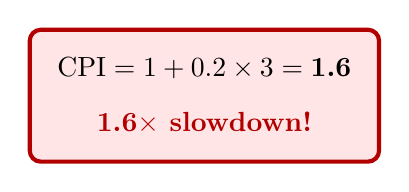
\begin{tikzpicture}
    \node[draw=red!70!black, line width=1.5pt, fill=red!10, rounded corners=4pt,
          inner sep=10pt, align=center] {
        $\text{CPI} = 1 + 0.2 \times 3 = \textbf{1.6}$\\[8pt]
        \textcolor{red!70!black}{\textbf{1.6$\times$ slowdown!}}
    };
\end{tikzpicture}
\end{column}
\end{columns}

\vspace{0.4cm}
\centering
$\text{CPI}_{\text{new}} = \text{CPI}_{\text{Ideal}} + \textit{avg}\left(\dfrac{\text{stall cycles}}{\text{instruction}}\right)$
\end{frame}

%% Slide: Control Hazard: Predict Not Taken
\begin{frame}{Control Hazard: Predict Not Taken}
\begin{columns}[T]
\begin{column}{0.58\textwidth}
\begin{itemize}
    \item Execute instructions from the fall-through path
    \begin{itemize}
        \item As if there is no branch
        \item If not-taken ($\sim$50\%), no penalty
    \end{itemize}
    \item If branch actually taken:
    \begin{itemize}
        \item Flush before state changes
        \item Fetch from correct path
    \end{itemize}
\end{itemize}
\end{column}
\begin{column}{0.38\textwidth}
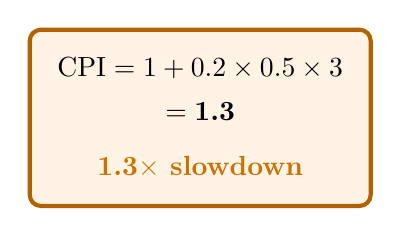
\begin{tikzpicture}
    \node[draw=myorange!70!black, line width=1.5pt, fill=myorange!10, rounded corners=4pt,
          inner sep=10pt, align=center] {
        $\text{CPI} = 1 + 0.2 \times 0.5 \times 3$\\[4pt]
        $= \textbf{1.3}$\\[8pt]
        \textcolor{myorange!80!black}{\textbf{1.3$\times$ slowdown}}
    };
\end{tikzpicture}
\end{column}
\end{columns}

\vspace{0.3cm}
\small
Assuming 20\% branches, $\sim$50\% taken on average
\end{frame}

%% Show overlay 5 (flush scenario - PPT slide 37) of Control Hazard on Branches
\againframe<5>{control-hazard}

%% Slide: Dynamic Branch Prediction
\begin{frame}{Dynamic Branch Prediction}
\begin{columns}[T]
\begin{column}{0.45\textwidth}
    \begin{itemize}
        \item \textbf{Branch Target Buffer} (BTB) that predicts (at fetch)
        \begin{itemize}
            \item Instruction is a branch
            \item Branch taken / not-taken
            \item Taken branch target
        \end{itemize}
        \vspace{0.3cm}
        \item BTB allocated at execute -- after all branch info is known
        \item BTB is looked up at instruction fetch
    \end{itemize}
\end{column}
\begin{column}{0.55\textwidth}
    \centering
    \btbdiagram
\end{column}
\end{columns}
\end{frame}


%% Slide: BTB
\begin{frame}{BTB}
\begin{columns}[T]
\begin{column}{0.48\textwidth}
\textcolor{myblue}{\textbf{(1) Allocation}} -- at Decode/EXE
\begin{itemize}
    \item Allocate branches after decode
    \item Not-taken branches need not be allocated
    \item BTB miss $\Rightarrow$ predict not-taken
\end{itemize}

\vspace{0.3cm}

\textcolor{myorange}{\textbf{(3) Update}} -- at EXE
\begin{itemize}
    \item Branch target
    \item Branch history (taken/not-taken)
\end{itemize}
\end{column}

\begin{column}{0.48\textwidth}
\textcolor{mygreen!80!black}{\textbf{(2) Prediction}} -- at Fetch
\begin{itemize}
    \item BTB lookup parallel to I\$ lookup
    \item BTB provides:
    \begin{itemize}
        \item Branch indication (BTB hit)
        \item Predicted target
        \item Predicted direction
        \item Branch type (cond./uncond.)
    \end{itemize}
\end{itemize}
\end{column}
\end{columns}
\end{frame}

%% Slide: Misprediction
\begin{frame}{Misprediction}
\begin{center}
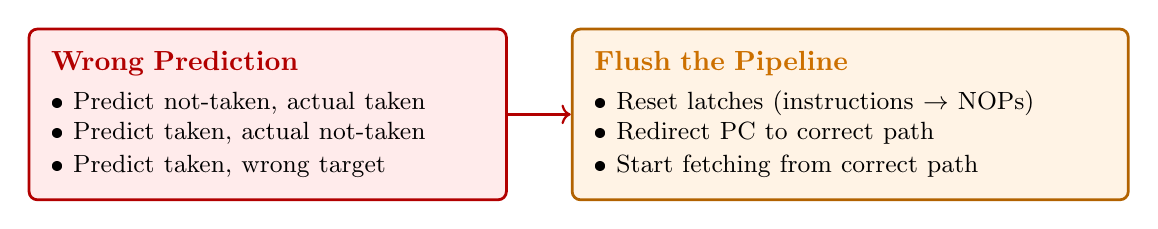
\begin{tikzpicture}
    % Wrong prediction box
    \node[draw=red!70!black, line width=1pt, fill=red!8, rounded corners=3pt,
          text width=5.5cm, align=left, inner sep=8pt] (wrong) {
        \textbf{\textcolor{red!70!black}{Wrong Prediction}}\\[3pt]
        \small
        \textbullet\ Predict not-taken, actual taken\\
        \textbullet\ Predict taken, actual not-taken\\
        \textbullet\ Predict taken, wrong target
    };

    % Flush box
    \node[draw=myorange!70!black, line width=1pt, fill=myorange!10, rounded corners=3pt,
          text width=6.5cm, align=left, inner sep=8pt, right=0.8cm of wrong] (flush) {
        \textbf{\textcolor{myorange!80!black}{Flush the Pipeline}}\\[3pt]
        \small
        \textbullet\ Reset latches (instructions $\rightarrow$ NOPs)\\
        \textbullet\ Redirect PC to correct path\\
        \textbullet\ Start fetching from correct path
    };

    % Arrow
    \draw[->, thick, red!70!black] (wrong.east) -- (flush.west);
\end{tikzpicture}
\end{center}

\vspace{0.2cm}

\begin{columns}[T]
\begin{column}{0.55\textwidth}
\textbf{Performance:} With prediction rate $P$:
\[
\text{CPI} = 1 + 0.2 \times (1{-}P) \times 3
\]
\textbf{Example:} $P = 70\%$ $\Rightarrow$ $\text{CPI} = \textbf{1.18}$
\end{column}
\begin{column}{0.42\textwidth}
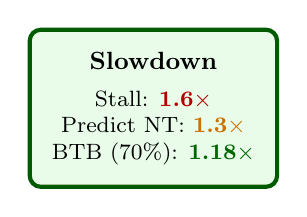
\begin{tikzpicture}
    \node[draw=mygreen!70!black, line width=1.5pt, fill=lightgreen!20, rounded corners=4pt,
          inner sep=8pt, align=center, font=\footnotesize] {
        \small\textbf{Slowdown}\\[4pt]
        Stall: \textcolor{red!70!black}{\textbf{1.6$\times$}}\\
        Predict NT: \textcolor{myorange!80!black}{\textbf{1.3$\times$}}\\
        BTB (70\%): \textcolor{mygreen!80!black}{\textbf{1.18$\times$}}
    };
\end{tikzpicture}
\end{column}
\end{columns}
\end{frame}


%% Slide: Adding a BTB to the Pipeline (based on lecture_06 style)
\begin{frame}{Adding a BTB to the Pipeline}
\begin{center}
\scalebox{0.58}{
\begin{circuitikz}[
    % Component styles matching lecture_06
    component/.style={draw, thick, minimum height=0.8cm},
    pipeline_reg/.style={draw, thick, fill=gray!20, minimum width=6mm, minimum height=5.8cm},
    stage_label/.style={draw, thick, fill=blue!60, text=white, font=\bfseries, minimum width=1.2cm, minimum height=0.5cm, text depth=0.25ex},
    imem_block/.style={muxdemux, muxdemux def={Lh=3, NL=3, Rh=3, NR=3, w=3.6, square pins=1},
                        external pins width=0, align=center, text depth=3ex, fill=yellow!20},
    bpu_block/.style={muxdemux, muxdemux def={Lh=3, NL=3, Rh=3, NR=3, w=3.6, square pins=1},
                        external pins width=0, align=center, text depth=6ex, fill=lightgreen!40},
    regfile/.style={muxdemux, muxdemux def={Lh=4, NL=4, Rh=4, NR=2, w=2.8, square pins=1},
                    external pins width=0, fill=cyan!20, align=center},
    alu_style/.style={muxdemux, muxdemux def={Lh=2.6, Rh=1.5, NL=2, NR=5, NB=1, w=1.3, inset w=0.5, inset Lh=2, inset Rh=0, square pins=1},
                     external pins width=0, fill=green!20, font=\scriptsize},
    adder/.style={muxdemux, muxdemux def={Lh=1.2, NL=2, Rh=0.6, NR=1, w=1, inset w=0.3, inset Lh=0.6, inset Rh=0, square pins=1},
                     external pins width=0, fill=cyan!20, font=\scriptsize},
    mux3/.style={muxdemux, muxdemux def={Lh=1, Rh=2, NL=1, NR=3, NT=2, w=0.8},
                 external pins width=0, fill=cyan!20},
    mux2/.style={muxdemux, muxdemux def={Lh=1.6, Rh=0.8, NL=2, NR=1, NB=1, w=0.8},
                 external pins width=0, fill=cyan!20},
    verify_comp/.style={muxdemux, muxdemux def={Lh=0.95, Rh=0.45, NL=2, NR=1, w=0.65, inset w=0.22, inset Lh=0.7, inset Rh=0, square pins=1},
                       external pins width=0, fill=red!30, font=\scriptsize},
    arrow/.style={->, >=stealth, thick},
    data_path/.style={arrow, black},
    bpu_path/.style={arrow, mygreen!70!black},
    repair_path/.style={arrow, red!70!black},
    verify_actual/.style={arrow, myorange!90!black},
    verify_flag/.style={arrow, red!70!black},
    line_label/.style={above, inner sep=1pt, font=\footnotesize},
    pred_target_label/.style={line_label, midway, text=mygreen!70!black},
    pred_dir_label/.style={line_label, midway, text=myorange!90!black},
    next_seq_label/.style={line_label, midway},
    repair_label/.style={line_label, text=red!70!black},
    lpin_label/.style={align=left, anchor=west, font=\tiny},
    rpin_label/.style={align=right, anchor=east, font=\tiny},
    data_connector/.style={circle, fill, inner sep=1.2pt},
    data_latch/.style={draw, thick, fill=cyan!20, minimum width=6mm, minimum height=0.3cm, inner sep=1pt, font=\tiny},
    inst_label/.style={draw, fill=orange!40, rounded corners=2pt, font=\scriptsize\ttfamily, inner sep=2pt},
    node distance=5mm and 5mm,
]

% IF Stage Components
\node[component, fill=yellow!30, minimum width=0.8cm] (PC) {IP};
\node[imem_block, right=of PC, anchor=blpin 2] (IMem) {Inst.\\Cache};
\node[adder, above=2mm of IMem.north, anchor=south] (PCadder) {+};
\node[mux3, anchor=south] (PCSrcMux) at ([yshift=13mm]IMem.north west) {};
\node[font=\scriptsize, left=5mm of PCadder.blpin 2] (four) {4};

% BPU in Fetch stage
\node[bpu_block, below=4mm of IMem] (BPU) {BTB};
\node[lpin_label] at (BPU.blpin 2) {IP};
\node[lpin_label] at (BPU.blpin 3) {allocate};
\node[rpin_label] at (BPU.rpin 2) {target};
\node[rpin_label] at (BPU.brpin 3) {dir};

% Pipeline register IF/ID
\node[pipeline_reg, right=8mm of IMem.brpin 2] (IFID) {};
\node[data_latch, minimum height=2cm] (Instruction) at (IMem.rpin 2 -| IFID) {\rotatebox{90}{Instruction}};

% ID Stage Components
\node[regfile, right=15mm of IFID] (RegFile) {\rotatebox{90}{Register File}};

% Sign Extend unit
\node[ellipse, draw, thick, fill=cyan!20, minimum width=0.3cm, minimum height=0.2cm, inner sep=0pt,
      font=\tiny, below=2mm of RegFile.south] (SignExt) {\rotatebox{90}{SignExt}};

% Pipeline register ID/EX
\node[pipeline_reg, right=8mm of RegFile.east |- IFID] (IDEX) {};

% EX Stage Components - ALU and MUX for immediate selection
\node[alu_style, anchor=blpin 1] (ALU) at ([xshift=2cm]RegFile.brpin 1 -| IDEX.east) {};
\node[mux2, anchor=rpin 1] (ALUMux) at ([xshift=-4mm]ALU.lpin 2) {};
\node[font=\scriptsize, below right=-2mm of ALU.blpin 1] {\rotatebox{-45}{ALU}};

% Target calculation adder
\node[adder, anchor=lpin 1] (TargetAdder) at ([xshift=-5mm]ALU.west |- PCadder.rpin 1) {+};

% Pipeline register EX/MEM
\node[pipeline_reg, right=12mm of ALU.east |- IDEX] (EXMEM) {};

% MEM Stage Components
\node[muxdemux, muxdemux def={Lh=4.1, NL=10, Rh=4.1, NR=10, w=2.8, square pins=1},
      external pins width=0, align=center, text depth=6.5ex, fill=yellow!20, anchor=lpin 5] (DMem) at ([xshift=1cm]ALU.brpin 4 -| EXMEM.east) {Data\\Cache};

% Verification comparators
\node[verify_comp, anchor=south] (DirComp) at ([yshift=5mm]DMem.north) {$\neq$};
\node[verify_comp, anchor=lpin 1] (TargetComp) at ([xshift=8mm]EXMEM.east |- PCSrcMux.rpin 2) {$\neq$};

% Logic gates for flush
\node[and port, number inputs=2, scale=0.26, fill=red!30, draw=red!70!black,
      line width=0.7pt, anchor=bin 1, external pins width=0] (MismatchAnd) at ([xshift=5mm]TargetComp.rpin 1) {};
\node[or port, number inputs=2, rotate=90, scale=0.26, fill=red!30, draw=red!70!black,
      line width=0.7pt, anchor=bin 1, external pins width=0] (FlushOr) at ([yshift=2mm, xshift=3mm]MismatchAnd.out) {};

% Actual outcome wires (orange) feeding comparators
\draw[arrow, orange!70!black] (ALU.brpin 2 -| EXMEM.east) -- ++(0.5,0) |- (DirComp.blpin 2);
\node[data_connector, fill=orange!70!black] (DirActualConn) at ([xshift=-3mm]DirComp.blpin 2) {};
\draw[arrow, orange!70!black] (DirActualConn) |- (MismatchAnd.bin 2);

% Comparator outputs and gating logic
\draw[verify_flag] (TargetComp.brpin 1) -- ++(1mm,0) |- (MismatchAnd.bin 1);
\draw[verify_flag] (MismatchAnd.bout) -| (FlushOr.bin 1);
\draw[verify_flag] (DirComp.brpin 1) -| (FlushOr.bin 2);

% Repair MUX
\node[muxdemux, muxdemux def={Lh=0.4, Rh=0.8, NL=1, NR=2, NB=1, w=0.5},
      external pins width=0, fill=blue!20, anchor=lpin 1] (RepairMux) at (PCSrcMux.rpin 1 -| TargetComp) {};

% Calc target to mux rpin 1
\coordinate (calc_target_mem_in) at (TargetAdder.brpin 1 -| EXMEM.east);
\coordinate (calc_target_top_right) at ([xshift=7mm]FlushOr.east |- RepairMux.rpin 1);
\node[data_connector, fill=green!60!black] (ActualTargetConn) at ([xshift=3mm]calc_target_mem_in) {};
\draw[arrow, green!60!black] (ActualTargetConn) |- (TargetComp.lpin 2);
\draw[arrow, green!60!black] (calc_target_mem_in) -| ([xshift=7mm]FlushOr.east) |- (RepairMux.rpin 1);

% Repair mux output to fetch mux
\draw[arrow, gray!50!black] (RepairMux.lpin 1) -- node[pos=0.5, line_label, text=gray!50!black] {repair IP} (PCSrcMux.rpin 1);

% Verification box background
\begin{scope}[on background layer]
    \node[draw=mygreen!70!black, line width=1pt, fill=lightgreen!35, rounded corners=4pt,
          fit=(TargetComp)(DirComp)(MismatchAnd)(FlushOr)(RepairMux)(ActualTargetConn)(calc_target_top_right),
          inner sep=2mm] (VerifyBox) {};
\end{scope}

% Pipeline register MEM/WB
\node[pipeline_reg, right=8mm of DMem.east |- EXMEM] (MEMWB) {};

% WB Stage
\node[mux2, anchor=lpin 1] at ([xshift=8mm]MEMWB.east |- DMem.rpin 5) (WBMux) {};

% Stage labels
\node[stage_label] (IF_label) at ([yshift=37mm]IMem.north) {Fetch};
\node[stage_label] (ID_label) at (IF_label -| RegFile) {Decode};
\node[stage_label] (EX_label) at (IF_label -| ALU) {Execute};
\node[stage_label] (MEM_label) at (IF_label -| DMem) {Memory};
\node[stage_label] (WB_label) at (IF_label -| WBMux) {WB};

% === Routing coordinates for pipeline signal propagation ===
% Predicted target coordinates
\coordinate (fetch_out_pred_target) at (IFID.west |- PCSrcMux.rpin 2);
\coordinate (decode_in_pred_target) at (IFID.east |- fetch_out_pred_target);
\coordinate (decode_out_pred_target) at (IDEX.west |- fetch_out_pred_target);
\coordinate (execute_in_pred_target) at (IDEX.east |- fetch_out_pred_target);
\coordinate (execute_out_pred_target) at (EXMEM.west |- fetch_out_pred_target);
\coordinate (mem_in_pred_target) at (execute_out_pred_target -| EXMEM.east);

% Predicted direction coordinates
\coordinate (fetch_out_pred_dir) at (IFID.north west |- DirComp.lpin 1);
\coordinate (decode_in_pred_dir) at (IFID.east |- fetch_out_pred_dir);
\coordinate (decode_out_pred_dir) at (IDEX.west |- fetch_out_pred_dir);
\coordinate (execute_in_pred_dir) at (IDEX.east |- fetch_out_pred_dir);
\coordinate (execute_out_pred_dir) at (EXMEM.west |- fetch_out_pred_dir);

% Next sequential address coordinates
\coordinate (fetch_out_next_seq) at (PCadder.brpin 1 -| IFID.west);
\coordinate (decode_in_next_seq) at (IFID.east |- fetch_out_next_seq);
\coordinate (decode_out_next_seq) at (IDEX.west |- fetch_out_next_seq);
\coordinate (execute_in_next_seq) at (IDEX.east |- fetch_out_next_seq);

% Target register coordinates
\coordinate (decode_out_target_reg) at ([yshift=-2mm]IDEX.west |- SignExt.south);
\coordinate (execute_in_target_reg) at (decode_out_target_reg -| IDEX.east);
\coordinate (execute_out_target_reg) at (decode_out_target_reg -| EXMEM.west);
\coordinate (mem_in_target_reg) at (decode_out_target_reg -| EXMEM.east);
\coordinate (mem_out_target_reg) at (decode_out_target_reg -| MEMWB.west);
\coordinate (wb_in_target_reg) at (decode_out_target_reg -| MEMWB.east);

% === Data paths ===
% MUX output to PC
\coordinate (IP_west_conn) at ([xshift=-5mm]PC.west);
\draw[data_path] (PCSrcMux.lpin 1) -| (IP_west_conn) -- (PC.west);
\draw[data_path] (PC.east) -- (IMem.blpin 2);

% Connector at IP west for BPU allocate
\node[data_connector] (IP_west_split) at (IP_west_conn) {};
\draw[data_path] (IP_west_split) |- (BPU.blpin 3);

% PC to BPU (IP input)
\node[data_connector] (PC_conn) at ([xshift=3mm]PC.east) {};
\draw[data_path] (PC_conn) |- (BPU.blpin 2);

% PC to adder
\draw[data_path] (PC_conn) |- (PCadder.blpin 1);
\draw[data_path] (four.east) -- (PCadder.blpin 2);

% === Next sequential address ===
\draw[data_path] (PCadder.brpin 1) -- ++(4mm,0) node[data_connector] (NextSeqConn) {} -- ++(0.1,0) |- (fetch_out_next_seq);
\draw[data_path] (NextSeqConn) |- (PCSrcMux.rpin 3);
\draw[data_path] (decode_in_next_seq) -- node[next_seq_label] {next sequential address} (decode_out_next_seq);
\coordinate (execute_out_next_seq) at ([yshift=2mm]execute_out_pred_dir -| EXMEM.west);
\draw[data_path] (execute_in_next_seq) -- ++(1,0) node[data_connector] (NextSeqExeConn) {} |- (TargetAdder.lpin 1);
\draw[data_path] (NextSeqExeConn) |- (execute_out_next_seq);
\coordinate (mem_in_next_seq) at (execute_out_next_seq -| EXMEM.east);
\draw[data_path] (mem_in_next_seq) -| ([xshift=4mm]FlushOr.east) |- (RepairMux.rpin 2);

% === Predicted target ===
\coordinate (target_joint) at ([xshift=2mm]BPU.rpin 2 |- PCSrcMux.rpin 2);
\draw[bpu_path] (BPU.brpin 2) -| (target_joint) node[data_connector] {} -- (fetch_out_pred_target);
\draw[bpu_path] (target_joint) -- (PCSrcMux.rpin 2);
\draw[bpu_path] (decode_in_pred_target) -- node[pred_target_label] {predicted target} (decode_out_pred_target);
\draw[bpu_path] (execute_in_pred_target) -- (execute_out_pred_target);
\draw[bpu_path] (mem_in_pred_target) -- (TargetComp.lpin 1);
\draw[verify_actual] (mem_in_pred_target) |- (DirComp.lpin 1);

% === Predicted direction ===
\coordinate (dir_joint) at ([xshift=5mm]BPU.brpin 3 |- fetch_out_pred_dir);
\draw[verify_actual] (BPU.brpin 3) -| (dir_joint) node[data_connector, fill=myorange!90!black] {} -- (fetch_out_pred_dir);
\draw[verify_actual] (dir_joint) |- ([yshift=2mm]PCSrcMux.tpin 2) -- (PCSrcMux.tpin 2);
\draw[verify_actual] (decode_in_pred_dir) -- node[pred_dir_label] {predicted direction} (decode_out_pred_dir);
\draw[verify_actual] (execute_in_pred_dir) -- (execute_out_pred_dir);

% IMem to IF/ID
\draw[data_path] (IMem.brpin 2) -- (IFID.west |- IMem.brpin 2);

% IF/ID to RegFile
\draw[data_path] (IFID.east |- RegFile.lpin 1) -- (RegFile.blpin 1);
\draw[data_path] (IFID.east |- RegFile.lpin 2) -- (RegFile.blpin 2);

% RegFile to ID/EX
\draw[data_path] (RegFile.brpin 1) -- (IDEX.west |- RegFile.brpin 1);
\draw[data_path] (RegFile.brpin 2) -- (IDEX.west |- RegFile.brpin 2);

% IF/ID to Sign Extend
\draw[data_path] (IFID.east |- SignExt) -- (SignExt.west);
% Sign Extend to ID/EX
\draw[data_path] (SignExt.east) -- (IDEX.west |- SignExt);

% ID/EX to ALU (top input direct, bottom through MUX)
\draw[data_path] (IDEX.east |- ALU.blpin 1) -- (ALU.blpin 1);
\coordinate (WriteDataJunction) at ([xshift=-3mm]ALUMux.lpin 1);
\draw[data_path] (IDEX.east |- ALUMux.lpin 1) -- (WriteDataJunction) node[data_connector] {} -- (ALUMux.blpin 1);
\draw[data_path] (WriteDataJunction) |- (EXMEM.west |- DMem.lpin 10);
\draw[data_path] (EXMEM.east |- DMem.lpin 10) -- (DMem.lpin 10);
\draw[data_path] (ALUMux.rpin 1) -- (ALU.blpin 2);

% SignExt through ID/EX to ALUMux and Target Adder
\coordinate (ImmJunction) at ([xshift=-7mm]ALUMux.lpin 2);
\draw[data_path] (SignExt -| IDEX.east) -| (ImmJunction) -- (ALUMux.lpin 2);
\node[data_connector] at (ImmJunction) {};
\draw[data_path] (ImmJunction) |- (TargetAdder.blpin 2);

% Target Adder to EX/MEM buffer
\draw[arrow, green!60!black] (TargetAdder.brpin 1) -- node[midway, line_label, text=green!60!black] {calc.\ target} (TargetAdder.brpin 1 -| EXMEM.west);

% ALU outputs to EX/MEM buffer
\coordinate (exmem_alu_zero) at (ALU.brpin 2 -| EXMEM.west);
\coordinate (exmem_alu_result) at (ALU.brpin 4 -| EXMEM.west);
\draw[arrow, orange!70!black] (ALU.brpin 2) -- node[midway, line_label, text=orange!70!black] {zero} (exmem_alu_zero);
\draw[data_path] (ALU.brpin 4) -- node[midway, line_label] {result} (exmem_alu_result);

% EX/MEM to DMem (addr)
\draw[data_path] (EXMEM.east |- DMem.lpin 5) -- (DMem.lpin 5);

% DMem to MEM/WB (read data)
\draw[data_path] (DMem.rpin 5) -- (MEMWB.west |- DMem.rpin 5);

% Instruction propagation through pipeline
\draw[data_path] ([yshift=8mm]Instruction.south east) -- ++(0.5,0) |- (decode_out_target_reg);
\draw[data_path] (execute_in_target_reg) -- (execute_out_target_reg);
\draw[data_path] (mem_in_target_reg) -- (mem_out_target_reg);
\draw[data_path] (wb_in_target_reg) -- ++(0.5,0) |- ([yshift=-5mm,xshift=-6mm]RegFile.west |- IDEX.south) |- (RegFile.blpin 3);

% MEM/WB to WB Mux
\draw[data_path] (MEMWB.east |- WBMux.lpin 1) -- (WBMux.blpin 1);

% Address path from DMem to WB Mux
\coordinate (AddrWB) at ([yshift=-3mm]DMem.south -| MEMWB.west);
\node[data_connector] (AddrConn) at ([xshift=-5mm]DMem.lpin 5) {};
\draw[data_path] (AddrConn) |- (AddrWB);
\draw[data_path] (AddrWB -| MEMWB.east) -- ++(0.5,0) |- (WBMux.lpin 2);

% WB Mux output to Register File write data
\draw[data_path] (WBMux.rpin 1) -- ++(0.5,0) |- ([xshift=-4mm,yshift=-8mm]IDEX.south -| RegFile.lpin 4) |- (RegFile.blpin 4);

% Flush signal from OR gate to fetch MUX
\coordinate (flush_line_y) at ([yshift=0.8cm]FlushOr.out);
\draw[repair_path, line width=1.5pt] (FlushOr.out) -- (flush_line_y) -| node[pos=0.2, repair_label] {flush and repair} (PCSrcMux.tpin 1);
\node[data_connector, fill=red!70!black] at (flush_line_y -| IDEX.north) {};
\draw[repair_path] (flush_line_y -| IDEX.north) -- (IDEX.north);
\node[data_connector, fill=red!70!black] at (flush_line_y -| IFID.north) {};
\draw[repair_path] (flush_line_y -| IFID.north) -- (IFID.north);

% Register File labels
\node[align=left, xshift=3mm, font=\tiny] at (RegFile.blpin 1) {read\\reg 1};
\node[align=left, xshift=3mm, font=\tiny] at (RegFile.blpin 2) {read\\reg 2};
\node[align=left, xshift=3mm, font=\tiny] at (RegFile.blpin 3) {write\\reg};
\node[align=left, xshift=3mm, font=\tiny] at (RegFile.blpin 4) {write\\data};
\node[align=right, xshift=-3mm, font=\tiny] at (RegFile.brpin 1) {read\\data 1};
\node[align=right, xshift=-3mm, font=\tiny] at (RegFile.brpin 2) {read\\data 2};

% Data Cache labels
\node[align=left, font=\tiny] at ([xshift=3mm,yshift=-1mm]DMem.lpin 5) {addr};
\node[align=left, font=\tiny] at ([xshift=3mm, yshift=2mm]DMem.lpin 10) {write\\data};
\node[align=right, font=\tiny] at ([xshift=-3mm,yshift=-2mm]DMem.rpin 5) {read\\data};

% === Animated callouts based on PowerPoint ===
\only<1>{
    \node[rectangle callout, draw=myorange!80!black, line width=1pt, fill=myorange!10,
          rounded corners=3pt, font=\scriptsize, align=center, inner sep=4pt,
          callout absolute pointer={([yshift=1mm]BPU.south)}, anchor=north]
          at ([yshift=-5mm]BPU.south) {
        Lookup current IP in I\$ and\\in BTB in parallel
    };
}
\only<2>{
    \node[rectangle callout, draw=myorange!80!black, line width=1pt, fill=myorange!10,
          rounded corners=3pt, font=\scriptsize, align=center, inner sep=4pt,
          callout absolute pointer={([yshift=1mm]BPU.south)}, anchor=north]
          at ([yshift=-5mm]BPU.south) {
        BTB provides predicted\\target and direction
    };
}
\only<3>{
    \node[rectangle callout, draw=myorange!80!black, line width=1pt, fill=myorange!10,
          rounded corners=3pt, font=\scriptsize, align=center, inner sep=4pt,
          callout absolute pointer={(IMem.south)}, anchor=north]
          at ([yshift=-5mm]IMem.south) {
        I\$ provides the\\instruction bytes
    };
}
\only<4>{
    % Combined verify callout pointing to verification box
    \node[rectangle callout, draw=purple!70!black, line width=1pt, fill=purple!10,
          rounded corners=3pt, font=\scriptsize, align=left, inner sep=4pt,
          callout absolute pointer={(VerifyBox.east)}]
          at ([xshift=2.5cm]VerifyBox.east) {
        Verify direction \& target
    };
}

% Program listing with border (right side)
\node[draw, thick, fill=white, rounded corners=3pt, inner sep=4pt,
      anchor=north west, font=\small\ttfamily, align=left]
      (ProgramListing) at ([xshift=5mm]WBMux.east |- IF_label.south) {
    \begin{tabular}{rl}
    0: & or \\
    4: & jcc 50 \\
    8: & and \\
    \multicolumn{2}{c}{...} \\
    50: & sub \\
    54: & mul \\
    58: & add \\
    \end{tabular}
};

% === Enhanced styles for visibility ===
% Coordinate for stage explanation box at bottom
\coordinate (StageExplainPos) at ([yshift=-20mm]BPU.south -| RegFile);

% Prominent instruction style on latches
\tikzset{
    latch_inst/.style={draw=blue!70!black, line width=1.5pt, fill=blue!15,
                       rounded corners=3pt, font=\small\bfseries\ttfamily, inner sep=4pt,
                       minimum height=5mm, text depth=0.5ex},
    latch_inst_highlight/.style={draw=red!70!black, line width=2pt, fill=yellow!30,
                       rounded corners=3pt, font=\small\bfseries\ttfamily, inner sep=4pt,
                       minimum height=5mm, text depth=0.5ex},
    latch_target/.style={draw=green!60!black, line width=1pt, fill=green!25,
                         rounded corners=3pt, font=\small\bfseries, inner sep=3pt},
    latch_dir/.style={draw=orange!60!black, line width=1pt, fill=orange!25,
                      rounded corners=3pt, font=\small\bfseries, inner sep=3pt},
    latch_nextseq/.style={draw=gray!60!black, line width=1pt, fill=gray!20,
                          rounded corners=3pt, font=\small\bfseries, inner sep=3pt},
    % Actual values from execution (for verification)
    latch_actual_dir/.style={draw=green!70!black, line width=1pt, fill=green!20,
                             rounded corners=3pt, font=\small\bfseries, inner sep=3pt},
    latch_actual_target/.style={draw=green!70!black, line width=1pt, fill=green!15,
                                rounded corners=3pt, font=\small\bfseries, inner sep=3pt},
    % IP value style
    ip_value/.style={font=\small\bfseries, text=blue!70!black},
    % Branch offset style
    branch_offset/.style={draw=cyan!60!black, line width=1pt, fill=cyan!15,
                          rounded corners=2pt, font=\scriptsize\bfseries, inner sep=2pt},
    stage_box/.style={draw=blue!50!black, line width=1.5pt, fill=blue!8,
                      rounded corners=6pt, font=\small, inner sep=8pt},
}

% === Animation: Instructions on latches + values + callouts ===
% Slide 1: or fetching, lookup BTB
\only<1>{
    % IP value below IP register
    \node[ip_value] at ([yshift=-3mm]PC.south) {4};
    % Instruction on IF/ID latch - bottom aligned with Instruction rectangle bottom
    \node[latch_inst] at (Instruction.south) {or};
    % Stage explanation - colorbox at bottom
    \node[stage_box, anchor=west] at (StageExplainPos) {
        \textcolor{blue!60!black}{\textbf{Fetch:}} Looking up IP=4 in I\$ and BTB in parallel
    };
}

% Slide 2: jcc fetching, BTB provides prediction
\only<2>{
    % IP value below IP register
    \node[ip_value] at ([yshift=-3mm]PC.south) {4};
    % Instruction on latch with branch offset below
    \node[latch_inst] (jcc2) at (Instruction.south) {jcc};
    \node[branch_offset, anchor=north] at (jcc2.south) {42};
    % Latch values - positioned relative to signal coordinates
    \node[latch_target] at (IFID.center |- fetch_out_pred_target) {50};
    \node[latch_dir] at ([yshift=2mm]IFID.center |- fetch_out_pred_dir) {taken};
    \node[latch_nextseq] at (IFID.center |- fetch_out_next_seq) {8};
    % Stage explanation
    \node[stage_box, anchor=west] at (StageExplainPos) {
        \textcolor{blue!60!black}{\textbf{Fetch:}} BTB hit! ~
        \colorbox{green!25}{\strut target=50}~
        \colorbox{orange!25}{\strut dir=taken}~
        \colorbox{gray!20}{\strut next=8}
    };
}

% Slide 3: sub fetching (from predicted path), jcc decoding
\only<3>{
    % IP value below IP register
    \node[ip_value] at ([yshift=-3mm]PC.south) {54};
    % Instructions on latches - using -| for consistent y-level
    \node[latch_inst] at (Instruction.south) {sub};
    \node[latch_inst] (jcc3) at (IDEX.center |- Instruction.south) {jcc};
    \node[branch_offset, anchor=north] at (jcc3.south) {42};
    % Latch values propagating - positioned relative to signal coordinates
    \node[latch_target] at (IDEX.center |- decode_out_pred_target) {50};
    \node[latch_dir] at ([yshift=2mm]IDEX.center |- decode_out_pred_dir) {taken};
    \node[latch_nextseq] at (IDEX.center |- decode_out_next_seq) {8};
    % Stage explanation
    \node[stage_box, anchor=west] at (StageExplainPos) {
        \textcolor{cyan!60!black}{\textbf{Decode:}} jcc decoded, prediction values propagate $\rightarrow$
    };
}

% Slide 4: mul fetching, sub decoding, jcc executing
\only<4>{
    % IP value below IP register
    \node[ip_value] at ([yshift=-3mm]PC.south) {58};
    % Instructions on latches - using -| for consistent y-level
    \node[latch_inst] at (Instruction.south) {mul};
    \node[latch_inst] at (IDEX.center |- Instruction.south) {sub};
    \node[latch_inst_highlight] (jcc4) at (EXMEM.center |- Instruction.south) {jcc};
    \node[branch_offset, anchor=north] at (jcc4.south) {42};
    % Predicted values - positioned relative to signal coordinates
    \node[latch_target] at (EXMEM.center |- execute_out_pred_target) {50};
    \node[latch_dir] at ([yshift=-1.5mm]EXMEM.center |- execute_out_pred_dir) {taken};
    \node[latch_nextseq] at ([yshift=1.5mm]EXMEM.center |- execute_out_next_seq) {8};
    % Actual values from execution (direction and calculated target)
    \node[latch_actual_dir] at (EXMEM.center |- exmem_alu_zero) {taken};
    \node[latch_actual_target] at (EXMEM.center |- calc_target_mem_in) {50};
    % Stage explanation
    \node[stage_box, anchor=west] at (StageExplainPos) {
        \textcolor{green!50!black}{\textbf{Execute:}} jcc executes $\rightarrow$ verify prediction at Memory
    };
    % Combined verify callout pointing to verification box
    \node[rectangle callout, draw=purple!70!black, line width=1.5pt, fill=purple!10,
          rounded corners=4pt, font=\small, align=left, inner sep=5pt,
          callout absolute pointer={(VerifyBox.east)}]
          at ([xshift=2.5cm]VerifyBox.east) {
        \textbf{Verify direction \& target}
    };
    % Mux callout explaining its role
    \node[rectangle callout, draw=blue!60!black, line width=1.5pt, fill=blue!10,
          rounded corners=4pt, font=\small, align=center, inner sep=5pt,
          callout absolute pointer={(PCSrcMux.north)}]
          at ([yshift=8mm]PCSrcMux.north) {
        next seq / target
    };
}

% Slide 5: add fetching, verification complete (OK)
\only<5>{
    % IP value below IP register
    \node[ip_value] at ([yshift=-3mm]PC.south) {62};
    % Instructions on latches - using -| for consistent y-level
    \node[latch_inst] at (Instruction.south) {add};
    \node[latch_inst] at (IDEX.center |- Instruction.south) {mul};
    \node[latch_inst] at (EXMEM.center |- Instruction.south) {sub};
    \node[latch_inst] at (MEMWB.center |- Instruction.south) {jcc};
    % Verification OK - prominent
    \node[draw=green!50!black, line width=2pt, fill=green!35, rounded corners=5pt,
          font=\normalsize\bfseries, inner sep=6pt, text=green!20!black]
          at (VerifyBox.center) {\checkmark~OK};
    % Stage explanation
    \node[draw=green!50!black, line width=1.5pt, fill=green!10, rounded corners=6pt,
          font=\small, inner sep=8pt, anchor=west] at (StageExplainPos) {
        \textcolor{green!40!black}{\textbf{Memory:}} Prediction correct! Pipeline continues normally~\checkmark
    };
}

\end{circuitikz}
}
\end{center}
\end{frame}

%% Slide: Predicted Taken Actual Not Taken
\begin{frame}{Predicted Taken, Actual Not Taken}
\begin{center}
\scalebox{0.58}{
\begin{circuitikz}[
    % Same styles as previous slide
    component/.style={draw, thick, minimum height=0.8cm},
    pipeline_reg/.style={draw, thick, fill=gray!20, minimum width=6mm, minimum height=5.8cm},
    stage_label/.style={draw, thick, fill=blue!60, text=white, font=\bfseries, minimum width=1.2cm, minimum height=0.5cm, text depth=0.25ex},
    imem_block/.style={muxdemux, muxdemux def={Lh=3, NL=3, Rh=3, NR=3, w=3.6, square pins=1},
                        external pins width=0, align=center, text depth=3ex, fill=yellow!20},
    bpu_block/.style={muxdemux, muxdemux def={Lh=3, NL=3, Rh=3, NR=3, w=3.6, square pins=1},
                        external pins width=0, align=center, text depth=6ex, fill=lightgreen!40},
    regfile/.style={muxdemux, muxdemux def={Lh=4, NL=4, Rh=4, NR=2, w=2.8, square pins=1},
                    external pins width=0, fill=cyan!20, align=center},
    alu_style/.style={muxdemux, muxdemux def={Lh=2.6, Rh=1.5, NL=2, NR=5, NB=1, w=1.3, inset w=0.5, inset Lh=2, inset Rh=0, square pins=1},
                     external pins width=0, fill=green!20, font=\scriptsize},
    adder/.style={muxdemux, muxdemux def={Lh=1.2, NL=2, Rh=0.6, NR=1, w=1, inset w=0.3, inset Lh=0.6, inset Rh=0, square pins=1},
                     external pins width=0, fill=cyan!20, font=\scriptsize},
    mux3/.style={muxdemux, muxdemux def={Lh=1, Rh=2, NL=1, NR=3, NT=2, w=0.8},
                 external pins width=0, fill=cyan!20},
    mux2/.style={muxdemux, muxdemux def={Lh=1.6, Rh=0.8, NL=2, NR=1, NB=1, w=0.8},
                 external pins width=0, fill=cyan!20},
    verify_comp/.style={muxdemux, muxdemux def={Lh=0.95, Rh=0.45, NL=2, NR=1, w=0.65, inset w=0.22, inset Lh=0.7, inset Rh=0, square pins=1},
                       external pins width=0, fill=red!30, font=\scriptsize},
    arrow/.style={->, >=stealth, thick},
    data_path/.style={arrow, black},
    bpu_path/.style={arrow, mygreen!70!black},
    repair_path/.style={arrow, red!70!black},
    verify_actual/.style={arrow, myorange!90!black},
    verify_flag/.style={arrow, red!70!black},
    line_label/.style={above, inner sep=1pt, font=\footnotesize},
    pred_target_label/.style={line_label, midway, text=mygreen!70!black},
    pred_dir_label/.style={line_label, midway, text=myorange!90!black},
    next_seq_label/.style={line_label, midway},
    repair_label/.style={line_label, text=red!70!black},
    lpin_label/.style={align=left, anchor=west, font=\tiny},
    rpin_label/.style={align=right, anchor=east, font=\tiny},
    data_connector/.style={circle, fill, inner sep=1.2pt},
    data_latch/.style={draw, thick, fill=cyan!20, minimum width=6mm, minimum height=0.3cm, inner sep=1pt, font=\tiny},
    inst_label/.style={draw, fill=orange!40, rounded corners=2pt, font=\scriptsize\ttfamily, inner sep=2pt},
    flush_label/.style={draw, fill=red!50, rounded corners=2pt, font=\scriptsize\ttfamily, inner sep=2pt, text=white},
    node distance=5mm and 5mm,
]

% IF Stage Components
\node[component, fill=yellow!30, minimum width=0.8cm] (PC) {IP};
\node[imem_block, right=of PC, anchor=blpin 2] (IMem) {Inst.\\Cache};
\node[adder, above=2mm of IMem.north, anchor=south] (PCadder) {+};
\node[mux3, anchor=south] (PCSrcMux) at ([yshift=13mm]IMem.north west) {};
\node[font=\scriptsize, left=5mm of PCadder.blpin 2] (four) {4};

% BPU in Fetch stage
\node[bpu_block, below=4mm of IMem] (BPU) {BTB};
\node[lpin_label] at (BPU.blpin 2) {IP};
\node[lpin_label] at (BPU.blpin 3) {allocate};
\node[rpin_label] at (BPU.rpin 2) {target};
\node[rpin_label] at (BPU.brpin 3) {dir};

% Pipeline register IF/ID
\node[pipeline_reg, right=8mm of IMem.brpin 2] (IFID) {};
\node[data_latch, minimum height=2cm] (Instruction) at (IMem.rpin 2 -| IFID) {\rotatebox{90}{Instruction}};

% ID Stage Components
\node[regfile, right=15mm of IFID] (RegFile) {\rotatebox{90}{Register File}};

% Sign Extend unit
\node[ellipse, draw, thick, fill=cyan!20, minimum width=0.3cm, minimum height=0.2cm, inner sep=0pt,
      font=\tiny, below=2mm of RegFile.south] (SignExt) {\rotatebox{90}{SignExt}};

% Pipeline register ID/EX
\node[pipeline_reg, right=8mm of RegFile.east |- IFID] (IDEX) {};

% EX Stage Components - ALU and MUX for immediate selection
\node[alu_style, anchor=blpin 1] (ALU) at ([xshift=2cm]RegFile.brpin 1 -| IDEX.east) {};
\node[mux2, anchor=rpin 1] (ALUMux) at ([xshift=-4mm]ALU.lpin 2) {};
\node[font=\scriptsize, below right=-2mm of ALU.blpin 1] {\rotatebox{-45}{ALU}};

% Target calculation adder
\node[adder, anchor=lpin 1] (TargetAdder) at ([xshift=-5mm]ALU.west |- PCadder.rpin 1) {+};

% Pipeline register EX/MEM
\node[pipeline_reg, right=12mm of ALU.east |- IDEX] (EXMEM) {};

% MEM Stage Components
\node[muxdemux, muxdemux def={Lh=4.1, NL=10, Rh=4.1, NR=10, w=2.8, square pins=1},
      external pins width=0, align=center, text depth=6.5ex, fill=yellow!20, anchor=lpin 5] (DMem) at ([xshift=1cm]ALU.brpin 4 -| EXMEM.east) {Data\\Cache};

% Verification comparators
\node[verify_comp, anchor=south] (DirComp) at ([yshift=5mm]DMem.north) {$\neq$};
\node[verify_comp, anchor=lpin 1] (TargetComp) at ([xshift=8mm]EXMEM.east |- PCSrcMux.rpin 2) {$\neq$};

% Logic gates for flush
\node[and port, number inputs=2, scale=0.26, fill=red!30, draw=red!70!black,
      line width=0.7pt, anchor=bin 1, external pins width=0] (MismatchAnd) at ([xshift=5mm]TargetComp.rpin 1) {};
\node[or port, number inputs=2, rotate=90, scale=0.26, fill=red!30, draw=red!70!black,
      line width=0.7pt, anchor=bin 1, external pins width=0] (FlushOr) at ([yshift=2mm, xshift=3mm]MismatchAnd.out) {};

% Actual outcome wires (orange) feeding comparators
\draw[arrow, orange!70!black] (ALU.brpin 2 -| EXMEM.east) -- ++(0.5,0) |- (DirComp.blpin 2);
\node[data_connector, fill=orange!70!black] (DirActualConn) at ([xshift=-3mm]DirComp.blpin 2) {};
\draw[arrow, orange!70!black] (DirActualConn) |- (MismatchAnd.bin 2);

% Comparator outputs and gating logic
\draw[verify_flag] (TargetComp.brpin 1) -- ++(1mm,0) |- (MismatchAnd.bin 1);
\draw[verify_flag] (MismatchAnd.bout) -| (FlushOr.bin 1);
\draw[verify_flag] (DirComp.brpin 1) -| (FlushOr.bin 2);

% Repair MUX
\node[muxdemux, muxdemux def={Lh=0.4, Rh=0.8, NL=1, NR=2, NB=1, w=0.5},
      external pins width=0, fill=blue!20, anchor=lpin 1] (RepairMux) at (PCSrcMux.rpin 1 -| TargetComp) {};

% Calc target to mux rpin 1
\coordinate (calc_target_mem_in) at (TargetAdder.brpin 1 -| EXMEM.east);
\coordinate (calc_target_top_right) at ([xshift=7mm]FlushOr.east |- RepairMux.rpin 1);
\node[data_connector, fill=green!60!black] (ActualTargetConn) at ([xshift=3mm]calc_target_mem_in) {};
\draw[arrow, green!60!black] (ActualTargetConn) |- (TargetComp.lpin 2);
\draw[arrow, green!60!black] (calc_target_mem_in) -| ([xshift=7mm]FlushOr.east) |- (RepairMux.rpin 1);

% Repair mux output to fetch mux
\draw[arrow, gray!50!black] (RepairMux.lpin 1) -- node[pos=0.5, line_label, text=gray!50!black] {repair IP} (PCSrcMux.rpin 1);

% Verification box background
\begin{scope}[on background layer]
    \node[draw=mygreen!70!black, line width=1pt, fill=lightgreen!35, rounded corners=4pt,
          fit=(TargetComp)(DirComp)(MismatchAnd)(FlushOr)(RepairMux)(ActualTargetConn)(calc_target_top_right),
          inner sep=2mm] (VerifyBox) {};
\end{scope}

% Pipeline register MEM/WB
\node[pipeline_reg, right=8mm of DMem.east |- EXMEM] (MEMWB) {};

% WB Stage
\node[mux2, anchor=lpin 1] at ([xshift=8mm]MEMWB.east |- DMem.rpin 5) (WBMux) {};

% Stage labels
\node[stage_label] (IF_label) at ([yshift=37mm]IMem.north) {Fetch};
\node[stage_label] (ID_label) at (IF_label -| RegFile) {Decode};
\node[stage_label] (EX_label) at (IF_label -| ALU) {Execute};
\node[stage_label] (MEM_label) at (IF_label -| DMem) {Memory};
\node[stage_label] (WB_label) at (IF_label -| WBMux) {WB};

% === Routing coordinates for pipeline signal propagation ===
% Predicted target coordinates
\coordinate (fetch_out_pred_target) at (IFID.west |- PCSrcMux.rpin 2);
\coordinate (decode_in_pred_target) at (IFID.east |- fetch_out_pred_target);
\coordinate (decode_out_pred_target) at (IDEX.west |- fetch_out_pred_target);
\coordinate (execute_in_pred_target) at (IDEX.east |- fetch_out_pred_target);
\coordinate (execute_out_pred_target) at (EXMEM.west |- fetch_out_pred_target);
\coordinate (mem_in_pred_target) at (execute_out_pred_target -| EXMEM.east);

% Predicted direction coordinates
\coordinate (fetch_out_pred_dir) at (IFID.north west |- DirComp.lpin 1);
\coordinate (decode_in_pred_dir) at (IFID.east |- fetch_out_pred_dir);
\coordinate (decode_out_pred_dir) at (IDEX.west |- fetch_out_pred_dir);
\coordinate (execute_in_pred_dir) at (IDEX.east |- fetch_out_pred_dir);
\coordinate (execute_out_pred_dir) at (EXMEM.west |- fetch_out_pred_dir);

% Next sequential address coordinates
\coordinate (fetch_out_next_seq) at (PCadder.brpin 1 -| IFID.west);
\coordinate (decode_in_next_seq) at (IFID.east |- fetch_out_next_seq);
\coordinate (decode_out_next_seq) at (IDEX.west |- fetch_out_next_seq);
\coordinate (execute_in_next_seq) at (IDEX.east |- fetch_out_next_seq);

% Target register coordinates
\coordinate (decode_out_target_reg) at ([yshift=-2mm]IDEX.west |- SignExt.south);
\coordinate (execute_in_target_reg) at (decode_out_target_reg -| IDEX.east);
\coordinate (execute_out_target_reg) at (decode_out_target_reg -| EXMEM.west);
\coordinate (mem_in_target_reg) at (decode_out_target_reg -| EXMEM.east);
\coordinate (mem_out_target_reg) at (decode_out_target_reg -| MEMWB.west);
\coordinate (wb_in_target_reg) at (decode_out_target_reg -| MEMWB.east);

% === Data paths ===
% MUX output to PC
\coordinate (IP_west_conn) at ([xshift=-5mm]PC.west);
\draw[data_path] (PCSrcMux.lpin 1) -| (IP_west_conn) -- (PC.west);
\draw[data_path] (PC.east) -- (IMem.blpin 2);

% Connector at IP west for BPU allocate
\node[data_connector] (IP_west_split) at (IP_west_conn) {};
\draw[data_path] (IP_west_split) |- (BPU.blpin 3);

% PC to BPU (IP input)
\node[data_connector] (PC_conn) at ([xshift=3mm]PC.east) {};
\draw[data_path] (PC_conn) |- (BPU.blpin 2);

% PC to adder
\draw[data_path] (PC_conn) |- (PCadder.blpin 1);
\draw[data_path] (four.east) -- (PCadder.blpin 2);

% === Next sequential address ===
\draw[data_path] (PCadder.brpin 1) -- ++(4mm,0) node[data_connector] (NextSeqConn) {} -- ++(0.1,0) |- (fetch_out_next_seq);
\draw[data_path] (NextSeqConn) |- (PCSrcMux.rpin 3);
\draw[data_path] (decode_in_next_seq) -- node[next_seq_label] {next sequential address} (decode_out_next_seq);
\coordinate (execute_out_next_seq) at ([yshift=2mm]execute_out_pred_dir -| EXMEM.west);
\draw[data_path] (execute_in_next_seq) -- ++(1,0) node[data_connector] (NextSeqExeConn) {} |- (TargetAdder.lpin 1);
\draw[data_path] (NextSeqExeConn) |- (execute_out_next_seq);
\coordinate (mem_in_next_seq) at (execute_out_next_seq -| EXMEM.east);
\draw[data_path] (mem_in_next_seq) -| ([xshift=4mm]FlushOr.east) |- (RepairMux.rpin 2);

% === Predicted target ===
\coordinate (target_joint) at ([xshift=2mm]BPU.rpin 2 |- PCSrcMux.rpin 2);
\draw[bpu_path] (BPU.brpin 2) -| (target_joint) node[data_connector] {} -- (fetch_out_pred_target);
\draw[bpu_path] (target_joint) -- (PCSrcMux.rpin 2);
\draw[bpu_path] (decode_in_pred_target) -- node[pred_target_label] {predicted target} (decode_out_pred_target);
\draw[bpu_path] (execute_in_pred_target) -- (execute_out_pred_target);
\draw[bpu_path] (mem_in_pred_target) -- (TargetComp.lpin 1);
\draw[verify_actual] (mem_in_pred_target) |- (DirComp.lpin 1);

% === Predicted direction ===
\coordinate (dir_joint) at ([xshift=5mm]BPU.brpin 3 |- fetch_out_pred_dir);
\draw[verify_actual] (BPU.brpin 3) -| (dir_joint) node[data_connector, fill=myorange!90!black] {} -- (fetch_out_pred_dir);
\draw[verify_actual] (dir_joint) |- ([yshift=2mm]PCSrcMux.tpin 2) -- (PCSrcMux.tpin 2);
\draw[verify_actual] (decode_in_pred_dir) -- node[pred_dir_label] {predicted direction} (decode_out_pred_dir);
\draw[verify_actual] (execute_in_pred_dir) -- (execute_out_pred_dir);

% IMem to IF/ID
\draw[data_path] (IMem.brpin 2) -- (IFID.west |- IMem.brpin 2);

% IF/ID to RegFile
\draw[data_path] (IFID.east |- RegFile.lpin 1) -- (RegFile.blpin 1);
\draw[data_path] (IFID.east |- RegFile.lpin 2) -- (RegFile.blpin 2);

% RegFile to ID/EX
\draw[data_path] (RegFile.brpin 1) -- (IDEX.west |- RegFile.brpin 1);
\draw[data_path] (RegFile.brpin 2) -- (IDEX.west |- RegFile.brpin 2);

% IF/ID to Sign Extend
\draw[data_path] (IFID.east |- SignExt) -- (SignExt.west);
% Sign Extend to ID/EX
\draw[data_path] (SignExt.east) -- (IDEX.west |- SignExt);

% ID/EX to ALU (top input direct, bottom through MUX)
\draw[data_path] (IDEX.east |- ALU.blpin 1) -- (ALU.blpin 1);
\coordinate (WriteDataJunction) at ([xshift=-3mm]ALUMux.lpin 1);
\draw[data_path] (IDEX.east |- WriteDataJunction) -- (WriteDataJunction) node[data_connector] {} -- (ALUMux.blpin 1);
\draw[data_path] (WriteDataJunction) |- (EXMEM.west |- DMem.lpin 10);
\draw[data_path] (EXMEM.east |- DMem.lpin 10) -- (DMem.lpin 10);
\draw[data_path] (ALUMux.rpin 1) -- (ALU.blpin 2);

% SignExt through ID/EX to ALUMux and Target Adder
\coordinate (ImmJunction) at ([xshift=-7mm]ALUMux.lpin 2);
\draw[data_path] (SignExt -| IDEX.east) -| (ImmJunction) -- (ALUMux.lpin 2);
\node[data_connector] at (ImmJunction) {};
\draw[data_path] (ImmJunction) |- (TargetAdder.blpin 2);

% Target Adder to EX/MEM buffer
\draw[arrow, green!60!black] (TargetAdder.brpin 1) -- node[midway, line_label, text=green!60!black] {calc.\ target} (TargetAdder.brpin 1 -| EXMEM.west);

% ALU outputs to EX/MEM buffer
\coordinate (exmem_alu_zero) at (ALU.brpin 2 -| EXMEM.west);
\coordinate (exmem_alu_result) at (ALU.brpin 4 -| EXMEM.west);
\draw[arrow, orange!70!black] (ALU.brpin 2) -- node[midway, line_label, text=orange!70!black] {zero} (exmem_alu_zero);
\draw[data_path] (ALU.brpin 4) -- node[midway, line_label] {result} (exmem_alu_result);

% EX/MEM to DMem (addr)
\draw[data_path] (EXMEM.east |- DMem.lpin 5) -- (DMem.lpin 5);

% DMem to MEM/WB (read data)
\draw[data_path] (DMem.rpin 5) -- (MEMWB.west |- DMem.rpin 5);

% Instruction propagation through pipeline
\draw[data_path] ([yshift=8mm]Instruction.south east) -- ++(0.5,0) |- (decode_out_target_reg);
\draw[data_path] (execute_in_target_reg) -- (execute_out_target_reg);
\draw[data_path] (mem_in_target_reg) -- (mem_out_target_reg);
\draw[data_path] (wb_in_target_reg) -- ++(0.5,0) |- ([yshift=-5mm,xshift=-6mm]RegFile.west |- IDEX.south) |- (RegFile.blpin 3);

% MEM/WB to WB Mux
\draw[data_path] (MEMWB.east |- WBMux.lpin 1) -- (WBMux.blpin 1);

% Address path from DMem to WB Mux
\coordinate (AddrWB) at ([yshift=-3mm]DMem.south -| MEMWB.west);
\node[data_connector] (AddrConn) at ([xshift=-5mm]DMem.lpin 5) {};
\draw[data_path] (AddrConn) |- (AddrWB);
\draw[data_path] (AddrWB -| MEMWB.east) -- ++(0.5,0) |- (WBMux.lpin 2);

% WB Mux output to Register File write data
\draw[data_path] (WBMux.rpin 1) -- ++(0.5,0) |- ([xshift=-4mm,yshift=-8mm]IDEX.south -| RegFile.lpin 4) |- (RegFile.blpin 4);

% Flush signal from OR gate to fetch MUX
\coordinate (flush_line_y) at ([yshift=0.8cm]FlushOr.out);
\draw[repair_path, line width=1.5pt] (FlushOr.out) -- (flush_line_y) -| node[pos=0.2, repair_label] {flush and repair} (PCSrcMux.tpin 1);
\node[data_connector, fill=red!70!black] at (flush_line_y -| IDEX.north) {};
\draw[repair_path] (flush_line_y -| IDEX.north) -- (IDEX.north);
\node[data_connector, fill=red!70!black] at (flush_line_y -| IFID.north) {};
\draw[repair_path] (flush_line_y -| IFID.north) -- (IFID.north);

% Register File labels
\node[align=left, xshift=3mm, font=\tiny] at (RegFile.blpin 1) {read\\reg 1};
\node[align=left, xshift=3mm, font=\tiny] at (RegFile.blpin 2) {read\\reg 2};
\node[align=left, xshift=3mm, font=\tiny] at (RegFile.blpin 3) {write\\reg};
\node[align=left, xshift=3mm, font=\tiny] at (RegFile.blpin 4) {write\\data};
\node[align=right, xshift=-3mm, font=\tiny] at (RegFile.brpin 1) {read\\data 1};
\node[align=right, xshift=-3mm, font=\tiny] at (RegFile.brpin 2) {read\\data 2};

% Data Cache labels
\node[align=left, font=\tiny] at ([xshift=3mm,yshift=-1mm]DMem.lpin 5) {addr};
\node[align=left, font=\tiny] at ([xshift=3mm, yshift=2mm]DMem.lpin 10) {write\\data};
\node[align=right, font=\tiny] at ([xshift=-3mm,yshift=-2mm]DMem.rpin 5) {read\\data};

% Program listing with border
\node[draw, thick, fill=white, rounded corners=3pt, inner sep=4pt,
      anchor=north west, font=\small\ttfamily, align=left]
      (ProgramListing) at ([xshift=5mm]WBMux.east |- IF_label.south) {
    \begin{tabular}{rl}
    0: & or \\
    4: & jcc 50 \\
    8: & and \\
    \multicolumn{2}{c}{...} \\
    50: & sub \\
    54: & mul \\
    \end{tabular}
};

% === Enhanced styles (same as first slide) ===
\coordinate (StageExplainPos) at ([yshift=-20mm]BPU.south -| RegFile);

\tikzset{
    latch_inst/.style={draw=blue!70!black, line width=1.5pt, fill=blue!15,
                       rounded corners=3pt, font=\small\bfseries\ttfamily, inner sep=4pt,
                       minimum height=5mm, text depth=0.5ex},
    latch_inst_highlight/.style={draw=red!70!black, line width=2pt, fill=yellow!30,
                       rounded corners=3pt, font=\small\bfseries\ttfamily, inner sep=4pt,
                       minimum height=5mm, text depth=0.5ex},
    latch_inst_flush/.style={draw=red!70!black, line width=2pt, fill=red!40,
                       rounded corners=3pt, font=\small\bfseries\ttfamily, inner sep=4pt, text=white,
                       minimum height=5mm, text depth=0.5ex},
    latch_inst_nop/.style={draw=gray!50!black, line width=1pt, fill=gray!25,
                       rounded corners=3pt, font=\small\ttfamily, inner sep=4pt, opacity=0.7,
                       minimum height=5mm, text depth=0.5ex},
    latch_inst_new/.style={draw=green!60!black, line width=2pt, fill=green!25,
                       rounded corners=3pt, font=\small\bfseries\ttfamily, inner sep=4pt,
                       minimum height=5mm, text depth=0.5ex},
    latch_target/.style={draw=green!60!black, line width=1pt, fill=green!25,
                         rounded corners=3pt, font=\small\bfseries, inner sep=3pt},
    latch_dir/.style={draw=orange!60!black, line width=1pt, fill=orange!25,
                      rounded corners=3pt, font=\small\bfseries, inner sep=3pt},
    latch_nextseq/.style={draw=gray!60!black, line width=1pt, fill=gray!20,
                          rounded corners=3pt, font=\small\bfseries, inner sep=3pt},
    % Actual values from execution (for verification)
    latch_actual_dir/.style={draw=green!70!black, line width=1pt, fill=green!20,
                             rounded corners=3pt, font=\small\bfseries, inner sep=3pt},
    latch_actual_target/.style={draw=green!70!black, line width=1pt, fill=green!15,
                                rounded corners=3pt, font=\small\bfseries, inner sep=3pt},
    % IP value and branch offset styles
    ip_value/.style={font=\small\bfseries, text=blue!70!black},
    branch_offset/.style={draw=cyan!60!black, line width=1pt, fill=cyan!15,
                          rounded corners=2pt, font=\scriptsize\bfseries, inner sep=2pt},
    stage_box/.style={draw=blue!50!black, line width=1.5pt, fill=blue!8,
                      rounded corners=6pt, font=\small, inner sep=8pt},
}

% === Animated misprediction scenario ===
% Slide 1: mul/sub fetched on wrong path, jcc executing, detecting mismatch
\only<1>{
    % IP value below IP register
    \node[ip_value] at ([yshift=-3mm]PC.south) {58};
    % Instructions on latches - using -| for consistent y-level
    \node[latch_inst] at (Instruction.south) {mul};
    \node[latch_inst] at (IDEX.center |- Instruction.south) {sub};
    \node[latch_inst_highlight] (jccM1) at (EXMEM.center |- Instruction.south) {jcc};
    \node[branch_offset, anchor=north] at (jccM1.south) {42};
    \node[latch_inst] at (MEMWB.center |- Instruction.south) {or};
    % Predicted values - positioned relative to signal coordinates
    \node[latch_target] at (EXMEM.center |- execute_out_pred_target) {50};
    \node[latch_dir] at (EXMEM.center |- execute_out_pred_dir) {taken};
    \node[latch_nextseq] at (EXMEM.center |- execute_out_next_seq) {8};
    % Actual values from execution (NOT taken - mismatch!)
    \node[latch_actual_dir, draw=red!70!black, fill=red!20] at (EXMEM.center |- exmem_alu_zero) {Not taken};
    \node[latch_actual_target] at (EXMEM.center |- calc_target_mem_in) {50};
    % Callout: Wrong direction detected
    \node[rectangle callout, draw=red!80!black, line width=1.5pt, fill=red!15,
          rounded corners=4pt, font=\small, align=center, inner sep=6pt,
          callout absolute pointer={(DirComp.east)}, text width=3cm]
          at ([xshift=2cm, yshift=-1cm]DirComp.east) {
        \textbf{Wrong direction!}\\Actual: Not Taken
    };
    % Stage explanation
    \node[draw=red!50!black, line width=1.5pt, fill=red!8, rounded corners=6pt,
          font=\small, inner sep=8pt, anchor=west] at (StageExplainPos) {
        \textcolor{red!60!black}{\textbf{Execute:}} jcc actual direction = Not Taken $\neq$ predicted (Taken)
    };
}

% Slide 2: Flush detected, repair IP selected
\only<2>{
    % IP value - being repaired to 8
    \node[ip_value, text=red!70!black] at ([yshift=-3mm]PC.south) {$\rightarrow$8};
    % Instructions - mul/sub being flushed - using -| for consistent y-level
    \node[latch_inst_flush] at (Instruction.south) {\sout{mul} $\to$ NOP};
    \node[latch_inst_flush] at (IDEX.center |- Instruction.south) {\sout{sub} $\to$ NOP};
    \node[latch_inst_highlight] at (EXMEM.center |- Instruction.south) {jcc};
    \node[latch_inst] at (MEMWB.center |- Instruction.south) {or};
    % Mismatch indicator
    \node[draw=red!70!black, line width=2pt, fill=red!50, rounded corners=5pt,
          font=\normalsize\bfseries, inner sep=6pt, text=white]
          at (VerifyBox.center) {$\neq$ FLUSH};
    % Callout: Repair IP
    \node[rectangle callout, draw=red!80!black, line width=1.5pt, fill=yellow!20,
          rounded corners=4pt, font=\small, align=center, inner sep=6pt,
          callout absolute pointer={(RepairMux.north)}, text width=3.5cm]
          at ([yshift=1.5cm,xshift=4cm]RepairMux.south) {
        \textbf{Repair IP} $\leftarrow$ 8\\(fall-through address)
    };
    % Stage explanation
    \node[draw=red!50!black, line width=1.5pt, fill=red!8, rounded corners=6pt,
          font=\small, inner sep=8pt, anchor=west] at (StageExplainPos) {
        \textcolor{red!60!black}{\textbf{Flush:}} Issue flush, select repair IP = 8 (next sequential), IF/ID and ID/EX $\to$ NOP
    };
}

% Slide 3: Pipeline flushed, bubbles inserted
\only<3>{
    % IP value - now at 8
    \node[ip_value] at ([yshift=-3mm]PC.south) {8};
    % Instructions - NOPs (bubbles) in flushed stages - using -| for consistent y-level
    \node[latch_inst_nop] at (Instruction.south) {NOP};
    \node[latch_inst_nop] at (IDEX.center |- Instruction.south) {NOP};
    \node[latch_inst] at (EXMEM.center |- Instruction.south) {jcc};
    \node[latch_inst] at (MEMWB.center |- Instruction.south) {or};
    % Stage explanation
    \node[draw=orange!50!black, line width=1.5pt, fill=orange!10, rounded corners=6pt,
          font=\small, inner sep=8pt, anchor=west] at (StageExplainPos) {
        \textcolor{orange!60!black}{\textbf{Flush:}} Pipeline flushed! IF/ID and ID/EX $\leftarrow$ NOP (bubbles)
    };
}

% Slide 4: Fetching from correct path
\only<4>{
    % IP value - at 8, fetching and
    \node[ip_value] at ([yshift=-3mm]PC.south) {8};
    % Instructions - and fetched from correct path - using -| for consistent y-level
    \node[latch_inst_new] at (Instruction.south) {and};
    \node[latch_inst_nop] at (IDEX.center |- Instruction.south) {--};
    \node[latch_inst_nop] at (EXMEM.center |- Instruction.south) {--};
    \node[latch_inst] at (MEMWB.center |- Instruction.south) {jcc};
    % Stage explanation
    \node[draw=green!50!black, line width=1.5pt, fill=green!10, rounded corners=6pt,
          font=\small, inner sep=8pt, anchor=west] at (StageExplainPos) {
        \textcolor{green!50!black}{\textbf{Recovery:}} Fetching ``and'' from correct path (IP=8). \textbf{3 cycle penalty}
    };
}

\end{circuitikz}
}
\end{center}
\end{frame}

%% Slide: Using The BTB
\begin{frame}{Using The BTB}
    \centering
    \tiny
    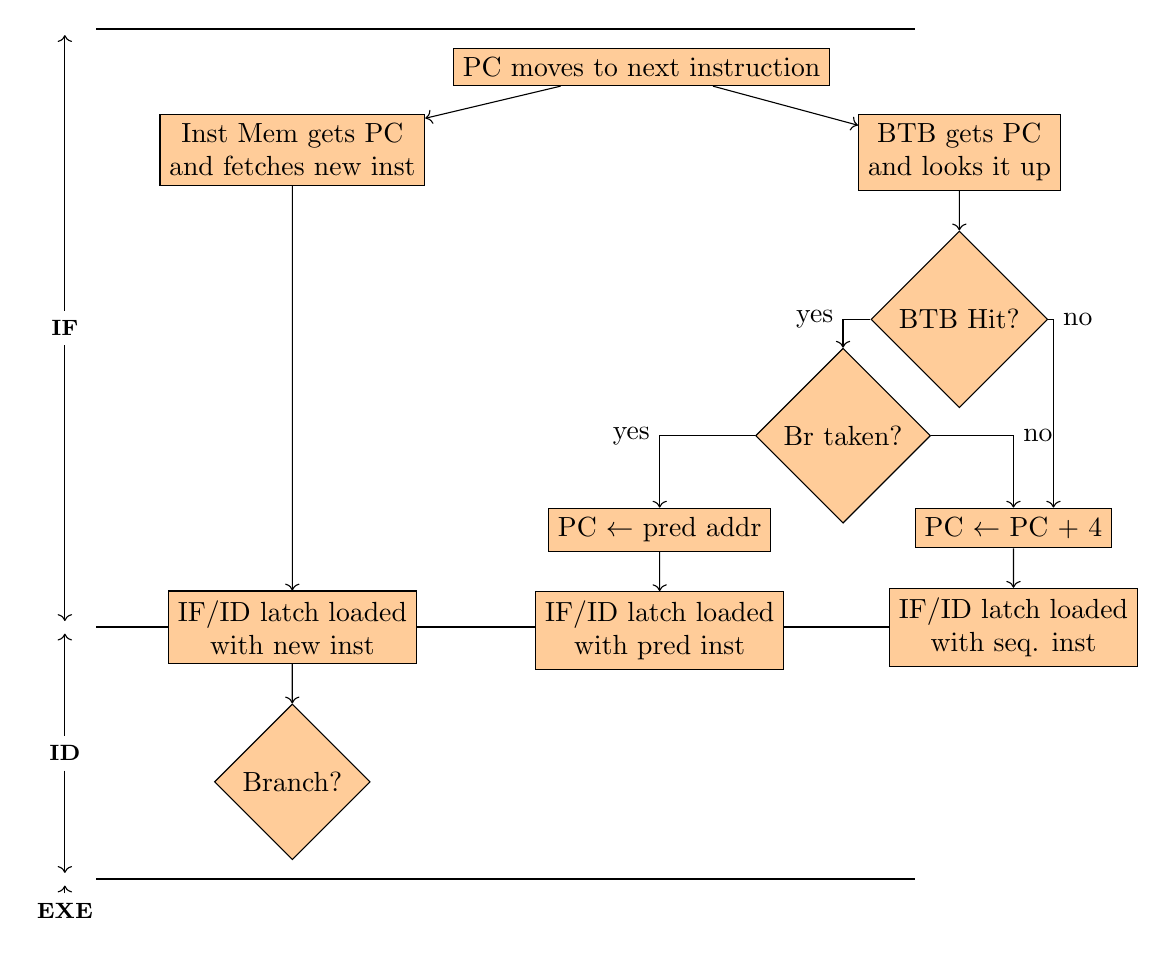
\begin{tikzpicture}[scale=0.8, node distance=0.5cm, remember picture,
        stage_label/.style={font=\footnotesize\bfseries}]

        % Shift flowchart to the right
        \begin{scope}[xshift=3cm]
        % Flowchart for BTB usage (drawn first)
        \node[draw, rectangle, fill=orange!40] (pc) {PC moves to next instruction};
        \node[draw, rectangle, fill=orange!40, below left=of pc, align=center] (imem) {Inst Mem gets PC\\and fetches new inst};
        \node[draw, rectangle, fill=orange!40, below right=of pc, align=center] (btb) {BTB gets PC\\and looks it up};
        \node[draw, diamond, fill=orange!40, below=of btb] (hit) {BTB Hit?};
        \node[draw, diamond, fill=orange!40, below left=of hit] (taken) {Br taken?};
        \node[draw, rectangle, fill=orange!40, below left=of taken] (pred) {PC $\leftarrow$ pred addr};
        \node[draw, rectangle, fill=orange!40, below right=of taken] (inc) {PC $\leftarrow$ PC + 4};
        \node[draw, rectangle, fill=orange!40, below=of pred, align=center] (predinst) {IF/ID latch loaded\\with pred inst};
        \node[draw, rectangle, fill=orange!40, below=of inc, align=center] (seqinst) {IF/ID latch loaded\\with seq. inst};
        \node[draw, rectangle, fill=orange!40, align=center] (new) at (seqinst -| imem) {IF/ID latch loaded\\with new inst};
        \node[draw, diamond, fill=orange!40, below=of new, align=center] (branch) {Branch?};

        \draw[->] (pc) -- (imem);
        \draw[->] (pc) -- (btb);
        \draw[->] (btb) -- (hit);
        \draw[->] (hit) -| node[left] {yes} (taken);
        \draw[->] (hit) -| node[right] {no} ([xshift=6.5cm]inc);
        \draw[->] (taken.west) -| node[left] {yes} (pred);
        \draw[->] (taken) -| node[right] {no} (inc);
        \draw[->] (pred) -- (predinst);
        \draw[->] (inc) -- (seqinst);
        \draw[->] (imem) -- (new);
        \draw[->] (new) -- (branch);

        % Pipeline stage labels with arrows (drawn on top)
        % Calculate boundary line positions based on actual nodes
        \coordinate (if_id_y) at ($(pc.north) + (0, 0.3)$);
        \coordinate (id_exe_y) at (new.center |- new.center);
        \coordinate (exe_mem_y) at ([yshift=-0.3cm]branch.south);

        % Find leftmost element
        \coordinate (leftmost) at (imem.west);
        \end{scope}

        % Position labels and lines relative to flowchart (outside shifted scope)
        \coordinate (label_x) at ($(leftmost) + (-1.5, 0)$);
        \coordinate (line_left) at ($(label_x) + (0.5, 0)$);
        \coordinate (line_right) at ($(line_left) + (13, 0)$);

        % Calculate midpoints for label positioning
        \coordinate (if_mid_y) at ($(if_id_y)!0.5!(id_exe_y)$);
        \coordinate (id_mid_y) at ($(id_exe_y)!0.5!(exe_mem_y)$);
        \coordinate (exe_mid_y) at ($(exe_mem_y) + (0, -0.5)$);

        % IF label and arrows (positioned at midpoint between if_id_y and id_exe_y)
        \node[stage_label] (if_label) at (label_x |- if_mid_y) {IF};
        \draw[->] (if_label.north) -- ($(if_label.north |- if_id_y) + (0, -0.1)$);
        \draw[->] (if_label.south) -- ($(if_label.south |- id_exe_y) + (0, 0.1)$);

        % ID label and arrows (positioned at midpoint between id_exe_y and exe_mem_y)
        \node[stage_label] (id_label) at (label_x |- id_mid_y) {ID};
        \draw[->] (id_label.north) -- ($(id_label.north |- id_exe_y) + (0, -0.1)$);
        \draw[->] (id_label.south) -- ($(id_label.south |- exe_mem_y) + (0, 0.1)$);

        % EXE label and arrow (positioned below exe_mem_y)
        \node[stage_label] (exe_label) at (label_x |- exe_mid_y) {EXE};
        \draw[->] (exe_label.north) -- ($(exe_label.north |- exe_mem_y) + (0, -0.1)$);

        % Draw horizontal lines (behind everything else by drawing them last but with background layer)
        \begin{scope}[on background layer]
            \draw[thick] (line_left |- if_id_y) -- (line_right |- if_id_y);
            \draw[thick] (line_left |- id_exe_y) -- (line_right |- id_exe_y);
            \draw[thick] (line_left |- exe_mem_y) -- (line_right |- exe_mem_y);
        \end{scope}
    \end{tikzpicture}
\end{frame}

%% Slide: Using The BTB (cont.)
\begin{frame}{Using The BTB (cont.)}
    \centering
    \tiny
    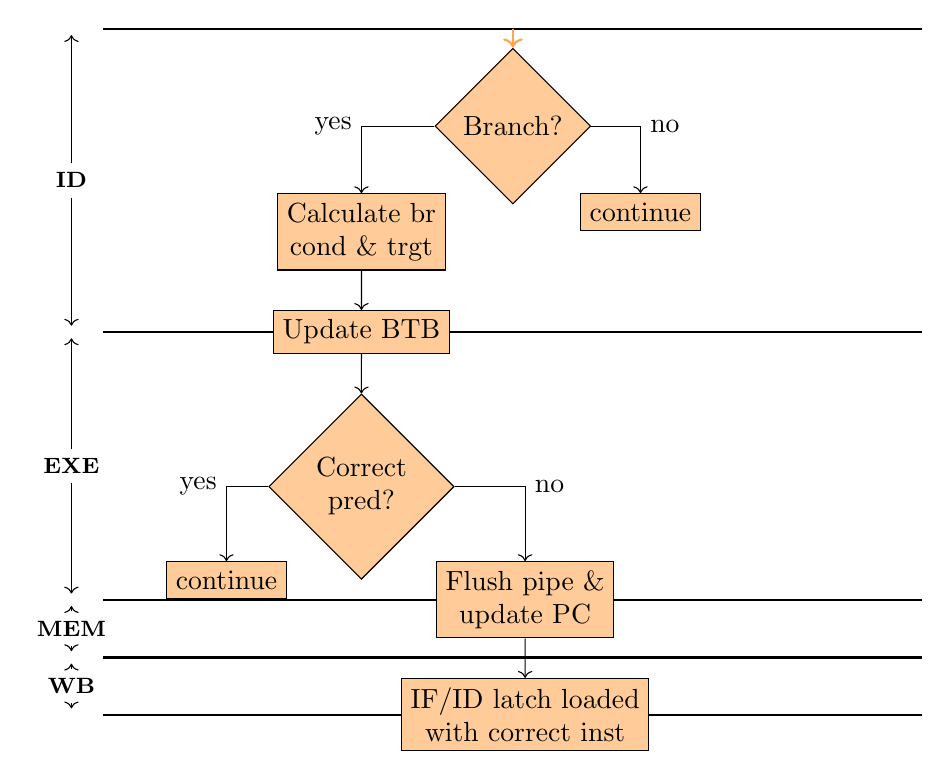
\begin{tikzpicture}[scale=0.8, node distance=0.5cm, remember picture,
        stage_label/.style={font=\footnotesize\bfseries}]

        % Shift flowchart to the right
        \begin{scope}[xshift=1cm]
        % Continuation of BTB flowchart (drawn first)
        \node[draw, diamond, fill=orange!40] (branch) {Branch?};
        \node[draw, rectangle, fill=orange!40, below left=of branch, align=center] (calc) {Calculate br\\cond \& trgt};
        \node[draw, rectangle, fill=orange!40, below right=of branch] (continue1) {continue};
        \node[draw, rectangle, fill=orange!40, below=of calc] (update) {Update BTB};
        \node[draw, diamond, fill=orange!40, below=of update, align=center] (correct) {Correct\\pred?};
        \node[draw, rectangle, fill=orange!40, below right=of correct, align=center] (flush) {Flush pipe \&\\update PC};
        \node[draw, rectangle, fill=orange!40, below left=of correct] (continue2) {continue};
        \node[draw, rectangle, fill=orange!40, below=of flush, align=center] (correctinst) {IF/ID latch loaded\\with correct inst};

        \draw[->] (branch) -| node[left] {yes} (calc);
        \draw[->] (branch) -| node[right] {no} (continue1);
        \draw[->] (calc) -- (update);
        \draw[->] (update) -- (correct);
        \draw[->] (correct) -| node[right] {no} (flush);
        \draw[->] (correct) -| node[left] {yes} (continue2);
        \draw[->] (flush) -- (correctinst);

        % Pipeline stage labels with arrows (drawn on top)
        % Calculate boundary line positions based on actual nodes
        \coordinate (id_exe_y) at ([yshift=0.3cm]branch.north);
        \coordinate (exe_mem_y) at (update.center |- update.center);
        \coordinate (mem_wb_y) at (flush.center);
        \coordinate (wb_end_y) at ([yshift=-0.3cm]flush.south);
        \coordinate (end_y) at (correctinst.center |- correctinst.center);

        % Add short arrow into branch from id_exe line
        \draw[->, thick, orange!70] ([yshift=0.3cm]branch.north) -- (branch.north);

        % Find leftmost element
        \coordinate (leftmost) at (continue2.west);
        \end{scope}

        % Position labels and lines relative to flowchart (outside shifted scope)
        \coordinate (label_x) at ($(leftmost) + (-1.5, 0)$);
        \coordinate (line_left) at ($(label_x) + (0.5, 0)$);
        \coordinate (line_right) at ($(line_left) + (13, 0)$);

        % Calculate midpoints for label positioning
        \coordinate (id_mid_y) at ($(id_exe_y)!0.5!(exe_mem_y)$);
        \coordinate (exe_mid_y) at ($(exe_mem_y)!0.5!(mem_wb_y)$);
        \coordinate (mem_mid_y) at ($(mem_wb_y)!0.5!(wb_end_y)$);
        \coordinate (wb_mid_y) at ($(wb_end_y)!0.5!(end_y)$);

        % ID label and arrows (positioned at midpoint between id_exe_y and exe_mem_y)
        \node[stage_label] (id_label) at (label_x |- id_mid_y) {ID};
        \draw[->] (id_label.north) -- ($(id_label.north |- id_exe_y) + (0, -0.1)$);
        \draw[->] (id_label.south) -- ($(id_label.south |- exe_mem_y) + (0, 0.1)$);

        % EXE label and arrows (positioned at midpoint between exe_mem_y and mem_wb_y)
        \node[stage_label] (exe_label) at (label_x |- exe_mid_y) {EXE};
        \draw[->] (exe_label.north) -- ($(exe_label.north |- exe_mem_y) + (0, -0.1)$);
        \draw[->] (exe_label.south) -- ($(exe_label.south |- mem_wb_y) + (0, 0.1)$);

        % MEM label and arrows (positioned at midpoint between mem_wb_y and wb_end_y)
        \node[stage_label] (mem_label) at (label_x |- mem_mid_y) {MEM};
        \draw[->] (mem_label.north) -- ($(mem_label.north |- mem_wb_y) + (0, -0.1)$);
        \draw[->] (mem_label.south) -- ($(mem_label.south |- wb_end_y) + (0, 0.1)$);

        % WB label and arrows (positioned at midpoint between wb_end_y and end_y)
        \node[stage_label] (wb_label) at (label_x |- wb_mid_y) {WB};
        \draw[->] (wb_label.north) -- ($(wb_label.north |- wb_end_y) + (0, -0.1)$);
        \draw[->] (wb_label.south) -- ($(wb_label.south |- end_y) + (0, 0.1)$);

        % Draw horizontal lines (behind everything else by drawing them last but with background layer)
        \begin{scope}[on background layer]
            \draw[thick] (line_left |- id_exe_y) -- (line_right |- id_exe_y);
            \draw[thick] (line_left |- exe_mem_y) -- (line_right |- exe_mem_y);
            \draw[thick] (line_left |- mem_wb_y) -- (line_right |- mem_wb_y);
            \draw[thick] (line_left |- wb_end_y) -- (line_right |- wb_end_y);
            \draw[thick] (line_left |- end_y) -- (line_right |- end_y);
        \end{scope}
    \end{tikzpicture}
\end{frame}

%% Backup Slides

%% Backup Slides Separator
\begin{frame}[plain]
    \begin{center}
        \vfill
        {\Huge \textbf{Backup Slides}}
        \vfill
    \end{center}
\end{frame}

%% Slide: Control Signals
\begin{frame}{Control Signals}
    \centering
    \footnotesize
    \renewcommand{\arraystretch}{0.9}
    \begin{tabular}{|l|c|c|c|c|c|c|c|}
        \hline
        \rowcolor{gray!20}\textbf{func} & \textbf{10 0000} & \textbf{10 0010} & \multicolumn{5}{c|}{\textbf{Don't Care}} \\
        \hline
        \rowcolor{gray!20}\textbf{op} & \textbf{00 0000} & \textbf{00 0000} & \textbf{00 1101} & \textbf{10 0011} & \textbf{10 1011} & \textbf{00 0100} & \textbf{00 0010} \\
        \hline
        \rowcolor{gray!20} & \textbf{add} & \textbf{sub} & \textbf{ori} & \textbf{lw} & \textbf{sw} & \textbf{beq} & \textbf{jump} \\
        \hline
        \textbf{RegDst} & 1 & 1 & 0 & 0 & x & x & x \\
        \hline
        \textbf{ALUSrc} & 0 & 0 & 1 & 1 & 1 & 0 & x \\
        \hline
        \textbf{MemtoReg} & 0 & 0 & 0 & 1 & x & x & x \\
        \hline
        \textbf{RegWrite} & 1 & 1 & 1 & 1 & 0 & 0 & 0 \\
        \hline
        \textbf{MemWrite} & 0 & 0 & 0 & 0 & 1 & 0 & 0 \\
        \hline
        \textbf{Branch} & 0 & 0 & 0 & 0 & 0 & 1 & x \\
        \hline
        \textbf{Jump} & 0 & 0 & 0 & 0 & 0 & 0 & 1 \\
        \hline
        \textbf{ALUctr$\langle$2:0$\rangle$} & Add & Subtract & Or & Add & Add & Subtract & xxx \\
        \hline
    \end{tabular}
\end{frame}

%% Slide: Multi-Cycle Control
\begin{frame}{Multi-Cycle Control}
    \begin{itemize}
        \item \textbf{Pass control signals along just like the data}
    \end{itemize}

    \vspace{0.2cm}
    \centering
    \scriptsize
    \begin{tabular}{|l|c|c|c|c|c|c|c|c|c|}
        \hline
        \rowcolor{gray!20} & \multicolumn{4}{c|}{\textbf{Execution/Address Calculation}} & \multicolumn{2}{c|}{\textbf{Memory access stage}} & \multicolumn{3}{c|}{\textbf{stage control}} \\
        \rowcolor{gray!20} & \multicolumn{4}{c|}{\textbf{stage control lines}} & \multicolumn{2}{c|}{\textbf{control lines}} & \multicolumn{3}{c|}{\textbf{lines}} \\
        \hline
        \rowcolor{gray!20}\textbf{Instruction} & \textbf{Reg} & \textbf{ALU} & \textbf{ALU} & \textbf{ALU} & & \textbf{Mem} & \textbf{Mem} & \textbf{Reg} & \textbf{Mem to} \\
        \rowcolor{gray!20} & \textbf{Dst} & \textbf{Op1} & \textbf{Op0} & \textbf{Src} & \textbf{Branch} & \textbf{Read} & \textbf{Write} & \textbf{write} & \textbf{Reg} \\
        \hline
        R-format & 1 & 1 & 0 & 0 & 0 & 0 & 0 & 1 & 0 \\
        \hline
        lw & 0 & 0 & 0 & 1 & 0 & 1 & 0 & 1 & 1 \\
        \hline
        sw & X & 0 & 0 & 1 & 0 & 0 & 1 & 0 & X \\
        \hline
        beq & X & 0 & 1 & 0 & 1 & 0 & 0 & 0 & X \\
        \hline
    \end{tabular}

    \vspace{0.3cm}
    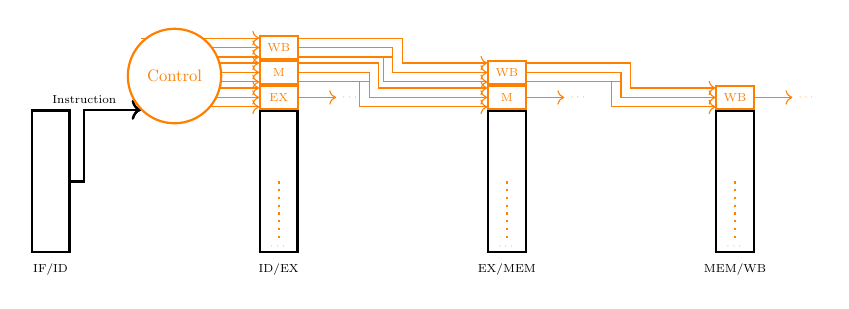
\begin{tikzpicture}[scale=0.6, transform shape]
        % Styles
        \tikzstyle{latch} = [draw, thick, minimum width=0.8cm, minimum height=3cm]
        \tikzstyle{control_box} = [draw, thick, orange, minimum width=0.8cm, minimum height=5mm,
                                    font=\scriptsize, align=center]

        % Pipeline register latches - rectangles with labels below
        \node[latch] (ifid) at (0,0) {};
        \node[below=1mm of ifid, font=\scriptsize] {IF/ID};

        \node[latch, anchor=west] (idex) at ([xshift=4cm]ifid.east) {};
        \node[below=1mm of idex, font=\scriptsize] {ID/EX};

        \node[latch, anchor=west] (exmem) at ([xshift=4cm]idex.east) {};
        \node[below=1mm of exmem, font=\scriptsize] {EX/MEM};

        \node[latch, anchor=west] (memwb) at ([xshift=4cm]exmem.east) {};
        \node[below=1mm of memwb, font=\scriptsize] {MEM/WB};

        % Control unit - positioned relative to IF/ID (define as coordinate first)
        \coordinate (control) at ([xshift=1.5cm]ifid.north east);

        % Instruction input
        \draw[->, thick] ([xshift=-2mm]control.west) -- (control.west);

        % Control signal boxes above ID/EX stage - adjacent using above=0cm of
        \node[control_box, anchor=south] (idex_ex) at (idex.north) {EX};
        \node[control_box, above=0cm of idex_ex] (idex_m) {M};
        \node[control_box, above=0cm of idex_m] (idex_wb) {WB};

        % Control signal boxes above EX/MEM stage - adjacent using above=0cm of
        \node[control_box, anchor=south] (exmem_m) at (exmem.north) {M};
        \node[control_box, above=0cm of exmem_m] (exmem_wb) {WB};

        % Control signal boxes above MEM/WB stage
        \node[control_box, anchor=south] (memwb_wb) at (memwb.north) {WB};

        % Dotted lines for data in latches
        \draw[orange, thick, dotted] (idex.center) -- +(0, -1.2) node[below, font=\tiny] {$\cdots$};
        \draw[orange, thick, dotted] (exmem.center) -- +(0, -1.2) node[below, font=\tiny] {$\cdots$};
        \draw[orange, thick, dotted] (memwb.center) -- +(0, -1.2) node[below, font=\tiny] {$\cdots$};

        % Arrow from IF/ID to Control unit
        \draw[->, thick] (ifid.east) -- ++(0.3, 0) |- node[above, font=\scriptsize] {Instruction} (control.west);

        % Control signals from Control unit to ID/EX - using |- with yshift
        \foreach \i in {-2mm, 0, 2mm} {
            \draw[->, orange] ([yshift=\i]control |- idex_wb) -- ([yshift=\i]idex_wb.west);
            \draw[->, orange] ([yshift=\i]control |- idex_m) -- ([yshift=\i]idex_m.west);
            \draw[->, orange] ([yshift=\i]control |- idex_ex) -- ([yshift=\i]idex_ex.west);
        }

        % WB signals propagating through stages
        \foreach \i in {-2mm, 0, 2mm} {
            \draw[->, orange] ([yshift=\i]idex_wb.east) -- ++(2,0) -- ++(\i,0) |- ([yshift=\i]exmem_wb.west);
            \draw[->, orange] ([yshift=\i]exmem_wb.east) -- ++(2,0) -- ++(\i,0) |- ([yshift=\i]memwb_wb.west);
        }
        
        \draw[->, orange] (memwb_wb.east) -- +(8mm,0) node[right, font=\tiny] {$\cdots$};

        % M signals propagating through stages
        \foreach \i in {-2mm, 0, 2mm} {
            \draw[->, orange] ([yshift=\i]idex_m.east) -- ++(1.5,0) -- ++(\i,0) |- ([yshift=\i]exmem_m.west);
        }
        \draw[->, orange] (exmem_m.east) -- +(8mm,0) node[right, font=\tiny] {$\cdots$};

        % EX signals
        \draw[->, orange] (idex_ex.east) -- +(8mm,0) node[right, font=\tiny] {$\cdots$};

        % Draw control unit on top with white fill to cover lines
        \node[draw, thick, ellipse, minimum width=1.5cm, minimum height=2cm, align=center, orange,
              fill=white, anchor=south west] at (control) {Control};
    \end{tikzpicture}
\end{frame}

%% Slide: Five Execution Steps
\begin{frame}{Five Execution Steps}
    \begin{itemize}
        \item \textbf{Instruction Fetch}
        \begin{itemize}
            \item Use PC to get instruction and put it in the Instruction Register.
            \item Increment the PC by 4 and put the result back in the PC.
            \item \texttt{IR = Memory[PC]; PC = PC + 4;}
        \end{itemize}

        \item \textbf{Instruction Decode and Register Fetch}
        \begin{itemize}
            \item Read registers rs and rt
            \item Compute the branch address
            \item \texttt{A = Reg[IR[25-21]]; B = Reg[IR[20-16]];}
            \item \texttt{ALUOut = PC + (sign-extend(IR[15-0]) << 2);}
            \item We aren't setting any control lines based on the instruction type
        \end{itemize}
    \end{itemize}
\end{frame}

%% Slide: Five Execution Steps (cont.)
\begin{frame}{Five Execution Steps (cont.)}
    \begin{itemize}
        \item \textbf{Execution} - ALU is performing one of three functions:
        \begin{itemize}
            \item \textbf{Memory Reference:} \texttt{ALUOut = A + sign-extend(IR[15-0]);}
            \item \textbf{R-type:} \texttt{ALUOut = A op B;}
            \item \textbf{Branch:} \texttt{if (A==B) PC = ALUOut;}
        \end{itemize}

        \item \textbf{Memory Access or R-type instruction completion}
        \item \textbf{Write-back step}
    \end{itemize}
\end{frame}

%% Slide: The Store Instruction
\begin{frame}{The Store Instruction}
    \begin{center}
    \textbf{Instruction Format:}

    \vspace{0.3cm}
    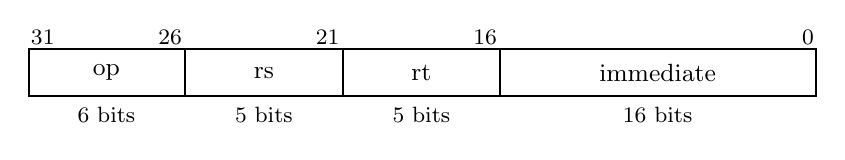
\begin{tikzpicture}
        % Main instruction box
        \node[draw, thick, minimum width=10cm, minimum height=0.6cm, inner sep=0pt] (box) {};

        % Field dividers
        \draw[thick] ([xshift=2cm]box.south west) -- ([xshift=2cm]box.north west);
        \draw[thick] ([xshift=4cm]box.south west) -- ([xshift=4cm]box.north west);
        \draw[thick] ([xshift=6cm]box.south west) -- ([xshift=6cm]box.north west);

        % Field labels (centered in each field)
        \node at ([xshift=1cm]box.west) {\small op};
        \node at ([xshift=3cm]box.west) {\small rs};
        \node at ([xshift=5cm]box.west) {\small rt};
        \node at ([xshift=8cm]box.west) {\small immediate};

        % Bit numbers at field boundaries (above)
        \node[anchor=south west, inner sep=1pt] at (box.north west) {\footnotesize 31};
        \node[anchor=south east, inner sep=1pt] at ([xshift=2cm]box.north west) {\footnotesize 26};
        \node[anchor=south east, inner sep=1pt] at ([xshift=4cm]box.north west) {\footnotesize 21};
        \node[anchor=south east, inner sep=1pt] at ([xshift=6cm]box.north west) {\footnotesize 16};
        \node[anchor=south east, inner sep=1pt] at (box.north east) {\footnotesize 0};

        % Bit widths (below)
        \node[anchor=north] at ([xshift=1cm]box.south west) {\footnotesize 6 bits};
        \node[anchor=north] at ([xshift=3cm]box.south west) {\footnotesize 5 bits};
        \node[anchor=north] at ([xshift=5cm]box.south west) {\footnotesize 5 bits};
        \node[anchor=north] at ([xshift=8cm]box.south west) {\footnotesize 16 bits};
    \end{tikzpicture}
    \end{center}

    \vspace{0.3cm}
    \textbf{Execution Steps:}
    \begin{itemize}
        \item Fetch instruction from memory: \texttt{mem[PC]}
        \item Calculate address: $\text{Addr} \leftarrow \text{R[rs]} + \text{SignExt(imm16)}$
        \item \textbf{Store:} $\textcolor{blue}{\text{Mem[Addr]} \leftarrow \text{R[rt]}}$
        \item Update PC: $\text{PC} \leftarrow \text{PC} + 4$
    \end{itemize}

    \vspace{0.2cm}
    \textbf{Example:} \texttt{sw rt, rs, imm16} \quad $\Rightarrow$ \quad $\text{Mem[R[rs]} + \text{SignExt(imm16)]} \leftarrow \text{R[rt]}$
\end{frame}

%% Slide: RAW Hazard: SW Solution
\begin{frame}{RAW Hazard: SW Solution}
    \begin{itemize}
        \item Have compiler avoid hazards by adding NOP instructions
        \item Problem: this really slows us down!
    \end{itemize}

    \vspace{0.5cm}
    \centering
    % TODO: Add figure for RAW hazard SW solution
    %\includegraphics[width=0.95\textwidth]{figures/raw_hazard_sw.png}
\end{frame}

%% Slide: Delayed Branch
\begin{frame}[fragile]{Delayed Branch}
    \vspace{-2mm}
    \begin{itemize}
        \item \textbf{Define branch to take place AFTER \textit{n} following instruction}
        \begin{itemize}
            \item HW executes \textit{n} instructions following the branch regardless of branch is taken or not
        \end{itemize}

        \item \textbf{SW puts in the \textit{n} slots following the branch instructions that need to be executed regardless of branch resolution}
        \begin{itemize}
            \item Instructions that are before the branch instruction, or
            \item Instructions from the converged path after the branch
        \end{itemize}

        \item \textbf{If cannot find independent instructions, put NOP}
    \end{itemize}

    \vspace{-0.7cm}
    \begin{columns}[T]
        \column{0.45\textwidth}
        \begin{tcolorbox}[title=Original Code, colback=blue!5, colframe=blue!50!black, fonttitle=\bfseries\small]
            \ttfamily\small
            \begin{tabular}[t]{@{}l@{}}
                ~~~r3 = 23 \\
                ~~~R4 = R3 + R5 \\
                ~~~If (r1==r2) goto x \\
                ~~~R1 = R4 + R5 \\
                X: R7 = R1
            \end{tabular}
        \end{tcolorbox}

        \column{0.45\textwidth}
        \begin{tcolorbox}[title=New Code, colback=green!5, colframe=green!50!black, fonttitle=\bfseries\small]
            \ttfamily\small
            \begin{tabular}[t]{@{}l@{}}
                ~~~If (r1==r2) goto x \\
                ~~~\textcolor{red}{r3 = 23} \\
                ~~~\textcolor{red}{R4 = R3 + R5} \\
                ~~~\textcolor{red}{NOP} \\
                ~~~R1 = R4 + R5 \\
                X: R7 = R1
            \end{tabular}
        \end{tcolorbox}
    \end{columns}
\end{frame}

%% Slide: Delayed Branch Performance
\begin{frame}{Delayed Branch Performance}
    \begin{itemize}
        \item Filling \textbf{1 delay slot is easy}, \textbf{2 is hard}, \textbf{3 is harder}
        \item Assume we can effectively fill \textbf{d\%} of the delayed slots
    \end{itemize}

    \vspace{0.5cm}
    \begin{center}
        \Large
        $\text{CPI}_{\text{new}} = 1 + 0.2 \times (3 \times (1-d))$
    \end{center}
    \vspace{0.5cm}

    \begin{itemize}
        \item For example, for $d=0.5$: \quad \textcolor{blue}{\textbf{$\text{CPI}_{\text{new}} = 1.3$}}
        \item \textbf{Problem: Mixing architecture with micro-architecture}
        \begin{itemize}
            \item New generations require more delay slots
            \item Causes \textbf{compatibility issues} between generations
        \end{itemize}
    \end{itemize}
\end{frame}

\end{document}